% This text is proprietary.
% It's a part of presentation made by myself.
% It may not used commercial.
% The noncommercial use such as private and study is free
% Sep. 2005
% Author: Sascha Frank
% University Freiburg
% www.informatik.uni-freiburg.de/~frank/


\documentclass{beamer}
%% \usetheme{Warsaw}

\usepackage{color}
\usepackage{booktabs}
\usepackage{tikz}
\usepackage{pgfplots}
\usepackage{graphicx}
\usepackage{caption}
\usepackage{subcaption}
\setbeamertemplate{navigation symbols}{}
\setbeamerfont{page number in head/foot}{size=\normalsize}
\setbeamertemplate{footline}[frame number]
\usetikzlibrary{positioning}
\AtBeginSection{\frame{\sectionpage}}
%% \AtBeginSubsection{\frame{\subsectionpage}}
\newcommand{\argmin}{\operatornamewithlimits{argmin}}
%% \DeclareMathOperator*{\argmin}{arg\,min}
%% \setbeamertemplate{caption}{\raggedright\insertcaption\par}
\captionsetup[figure]{labelformat=empty}% redefines the caption setup of the figures environment in the beamer class.
\captionsetup[subfigure]{labelformat=empty}% redefines the caption setup of the figures environment in the beamer class.




\newcommand*\nodestatecolor{green}
\newcommand*\scalefilter{0.7}
\newcommand*\initialstatetext{Previous State}
\newcommand*\initialstatecolor{yellow}

\tikzstyle{input}=[draw,fill=yellow,minimum width=2.6cm,thin]
\tikzstyle{method}=[draw,fill=pink,minimum width=1.8cm]
\tikzstyle{arr}=[-latex,ultra thick]
\tikzstyle{dummy}=[minimum width=2.6cm]


\title{Absolute scale velocity determination
combining visual and inertial
measurements for micro aerial
vehicles}
\subtitle{}
\date{June 24, 2015}
\author[Jacques Kaiser]{Jacques Kaiser\\{\small Supervised by Dr. Agostino Martinelli}}
 \institute{INRIA\\[\medskipamount]
      
\includegraphics[width=0.18\textwidth]{images/logoUJF.jpg} \hspace{1.5cm}
      
\includegraphics[width=0.18\textwidth]{images/logoINRIA.jpg} \hspace{1.5cm}
      
\includegraphics[width=0.18\textwidth]{images/logoINP.png}
 }
 %% \institute{INRIA}
 %% \titlegraphic{\includegraphics[width=\textwidth,height=.5\textheight]{someimage}}

\begin{document}

\maketitle

\section{Sensor fusion}

\begin{frame}{Micro aerial vehicles}
\includegraphics<1>[width=0.6\textwidth]{images/drone.png}
\includegraphics<2->[width=0.6\textwidth]{images/droneState.png}
%% \includegraphics<3->[width=0.6\textwidth]{images/dronePointState.png}

\onslide<3->

%drone is a rigid body - you can reduce it to a point
A basic state vector: $X =\left[\begin{array}{c}position \\ velocity \\ orientation\end{array}\right]$

%% \column{.5\textwidth}
%%         \begin{itemize}
%%         \item $r$ position;
%%         \item $\dot{r}$ velocity;
%%         \item $q$ orientation.
%%         \end{itemize}

\onslide<4->
\vspace{1em}
\textbf{The goal of sensor fusion is to recover the state $X$}
\end{frame}

\subsection{Filter based fusion}

\begin{frame}{Visual-inertial sensor fusion}

{\centering
\textbf{Filter based method}

\only<2->{\renewcommand*\nodestatecolor{yellow}}
%% \only<2->{\renewcommand*\scalefilter{0.7}}
\only<4->{\renewcommand*\initialstatecolor{blue!60}}
\only<4->{\renewcommand*\initialstatetext{Initial State}}

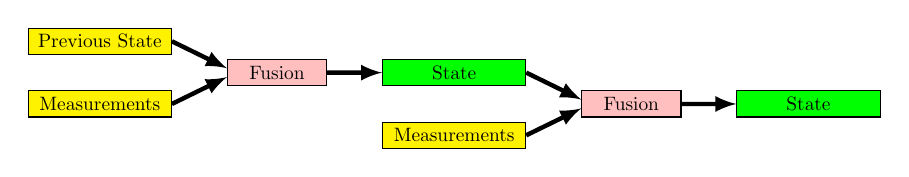
\begin{tikzpicture}[scale=\scalefilter, every node/.style={transform shape}]

\node (A) [input, fill=\initialstatecolor] {\initialstatetext};
\node (dummy1) [dummy, below=2mm of A] {};
\node (C) [input,below=2mm of dummy1] {Measurements};
\node (D) [method,right=of dummy1] {Fusion};
\node (E) [input, right=of D, fill=\nodestatecolor] {State};

\node<2-> (dummy2) [dummy, below=2mm of E] {};
\node<2-> (F) [input, below=2mm of dummy2] {Measurements};


\node<3-> (G) [method, right=of dummy2] {Fusion};
\node<3-> (H) [input, right=of G, fill=green] {State};

\draw[arr] (A.east) -- (D.175);
\draw[arr] (C.east) -- (D.185);
\draw[arr] (D.east) -- (E.west);
\draw<3->[arr] (E.east) -- (G.175);
\draw<3->[arr] (F.east) -- (G.185);
\draw<3->[arr] (G.east) -- (H.west);

\end{tikzpicture}
}

\onslide<4->
How to recover the \textbf{initial state}?

\onslide<5->
We need a \textbf{deterministic solution}

\vspace{0.5cm}
{\centering
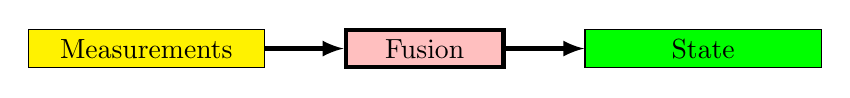
\begin{tikzpicture}
\tikzstyle{input}=[draw,fill=yellow,minimum width=3cm,thin]
\tikzstyle{method}=[draw,fill=pink,minimum width=2cm]
\tikzstyle{every path}=[-latex,ultra thick]
\node (C) [input] {Measurements};
\node (D) [method,right=of C] {Fusion};
\node (E) [input, right=of D, fill=green] {State};



\draw (C.east) -- (D.west);
\draw (D.east) -- (E.west);
\end{tikzpicture}
}

\end{frame}

\subsection{Deterministic solution}

\begin{frame}{Deterministic solutions in Computer Vision}

\begin{figure}
\centering
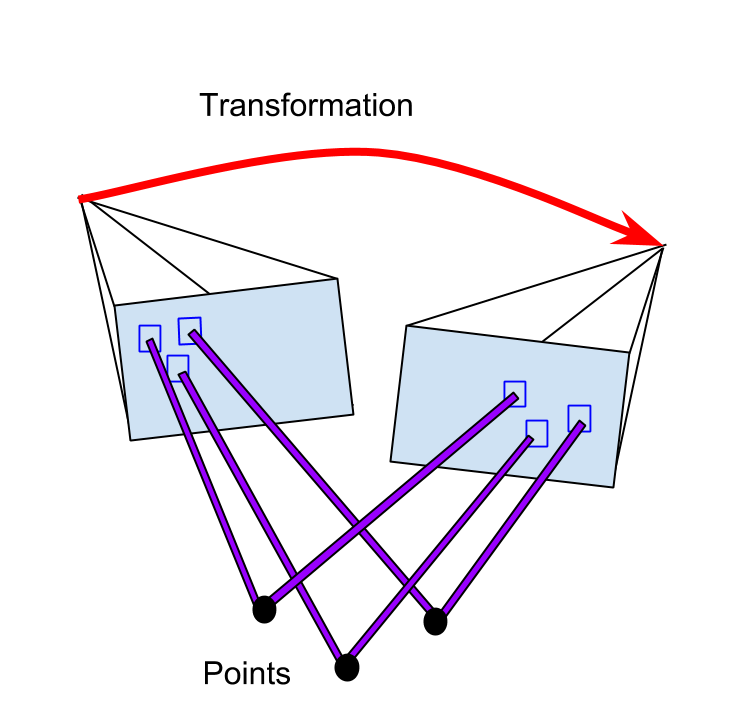
\includegraphics[width=0.5\textwidth]{images/directMethod.png}
\end{figure}

%% \onslide<2->
%% \begin{itemize}
%% \item 8-point algorithm;
%% \item sparse model-based image alignment;
%% \item ...
%% \end{itemize}

\onslide<2->

{\small
  But the relative \textbf{translation} and \textbf{distance to features} are recovered only \textbf{up to scale}
}

% Camera is an angle sensor
\end{frame}

\subsection{Absolute scale}

{ % all template changes are local to this group.
    \setbeamertemplate{navigation symbols}{}
    \begin{frame}[plain]{Absolute scale from visual measurements}
      How big is this building?
      \vspace{-2em}\begin{center}\includegraphics[width=\textwidth]{images/buildingDetour.png}\end{center}
     \end{frame}
}
{ % all template changes are local to this group.
    \setbeamertemplate{navigation symbols}{}
    \begin{frame}[plain]{Absolute scale from visual measurements}
      \vspace{1.03em}
      \vspace{-2em}\begin{center}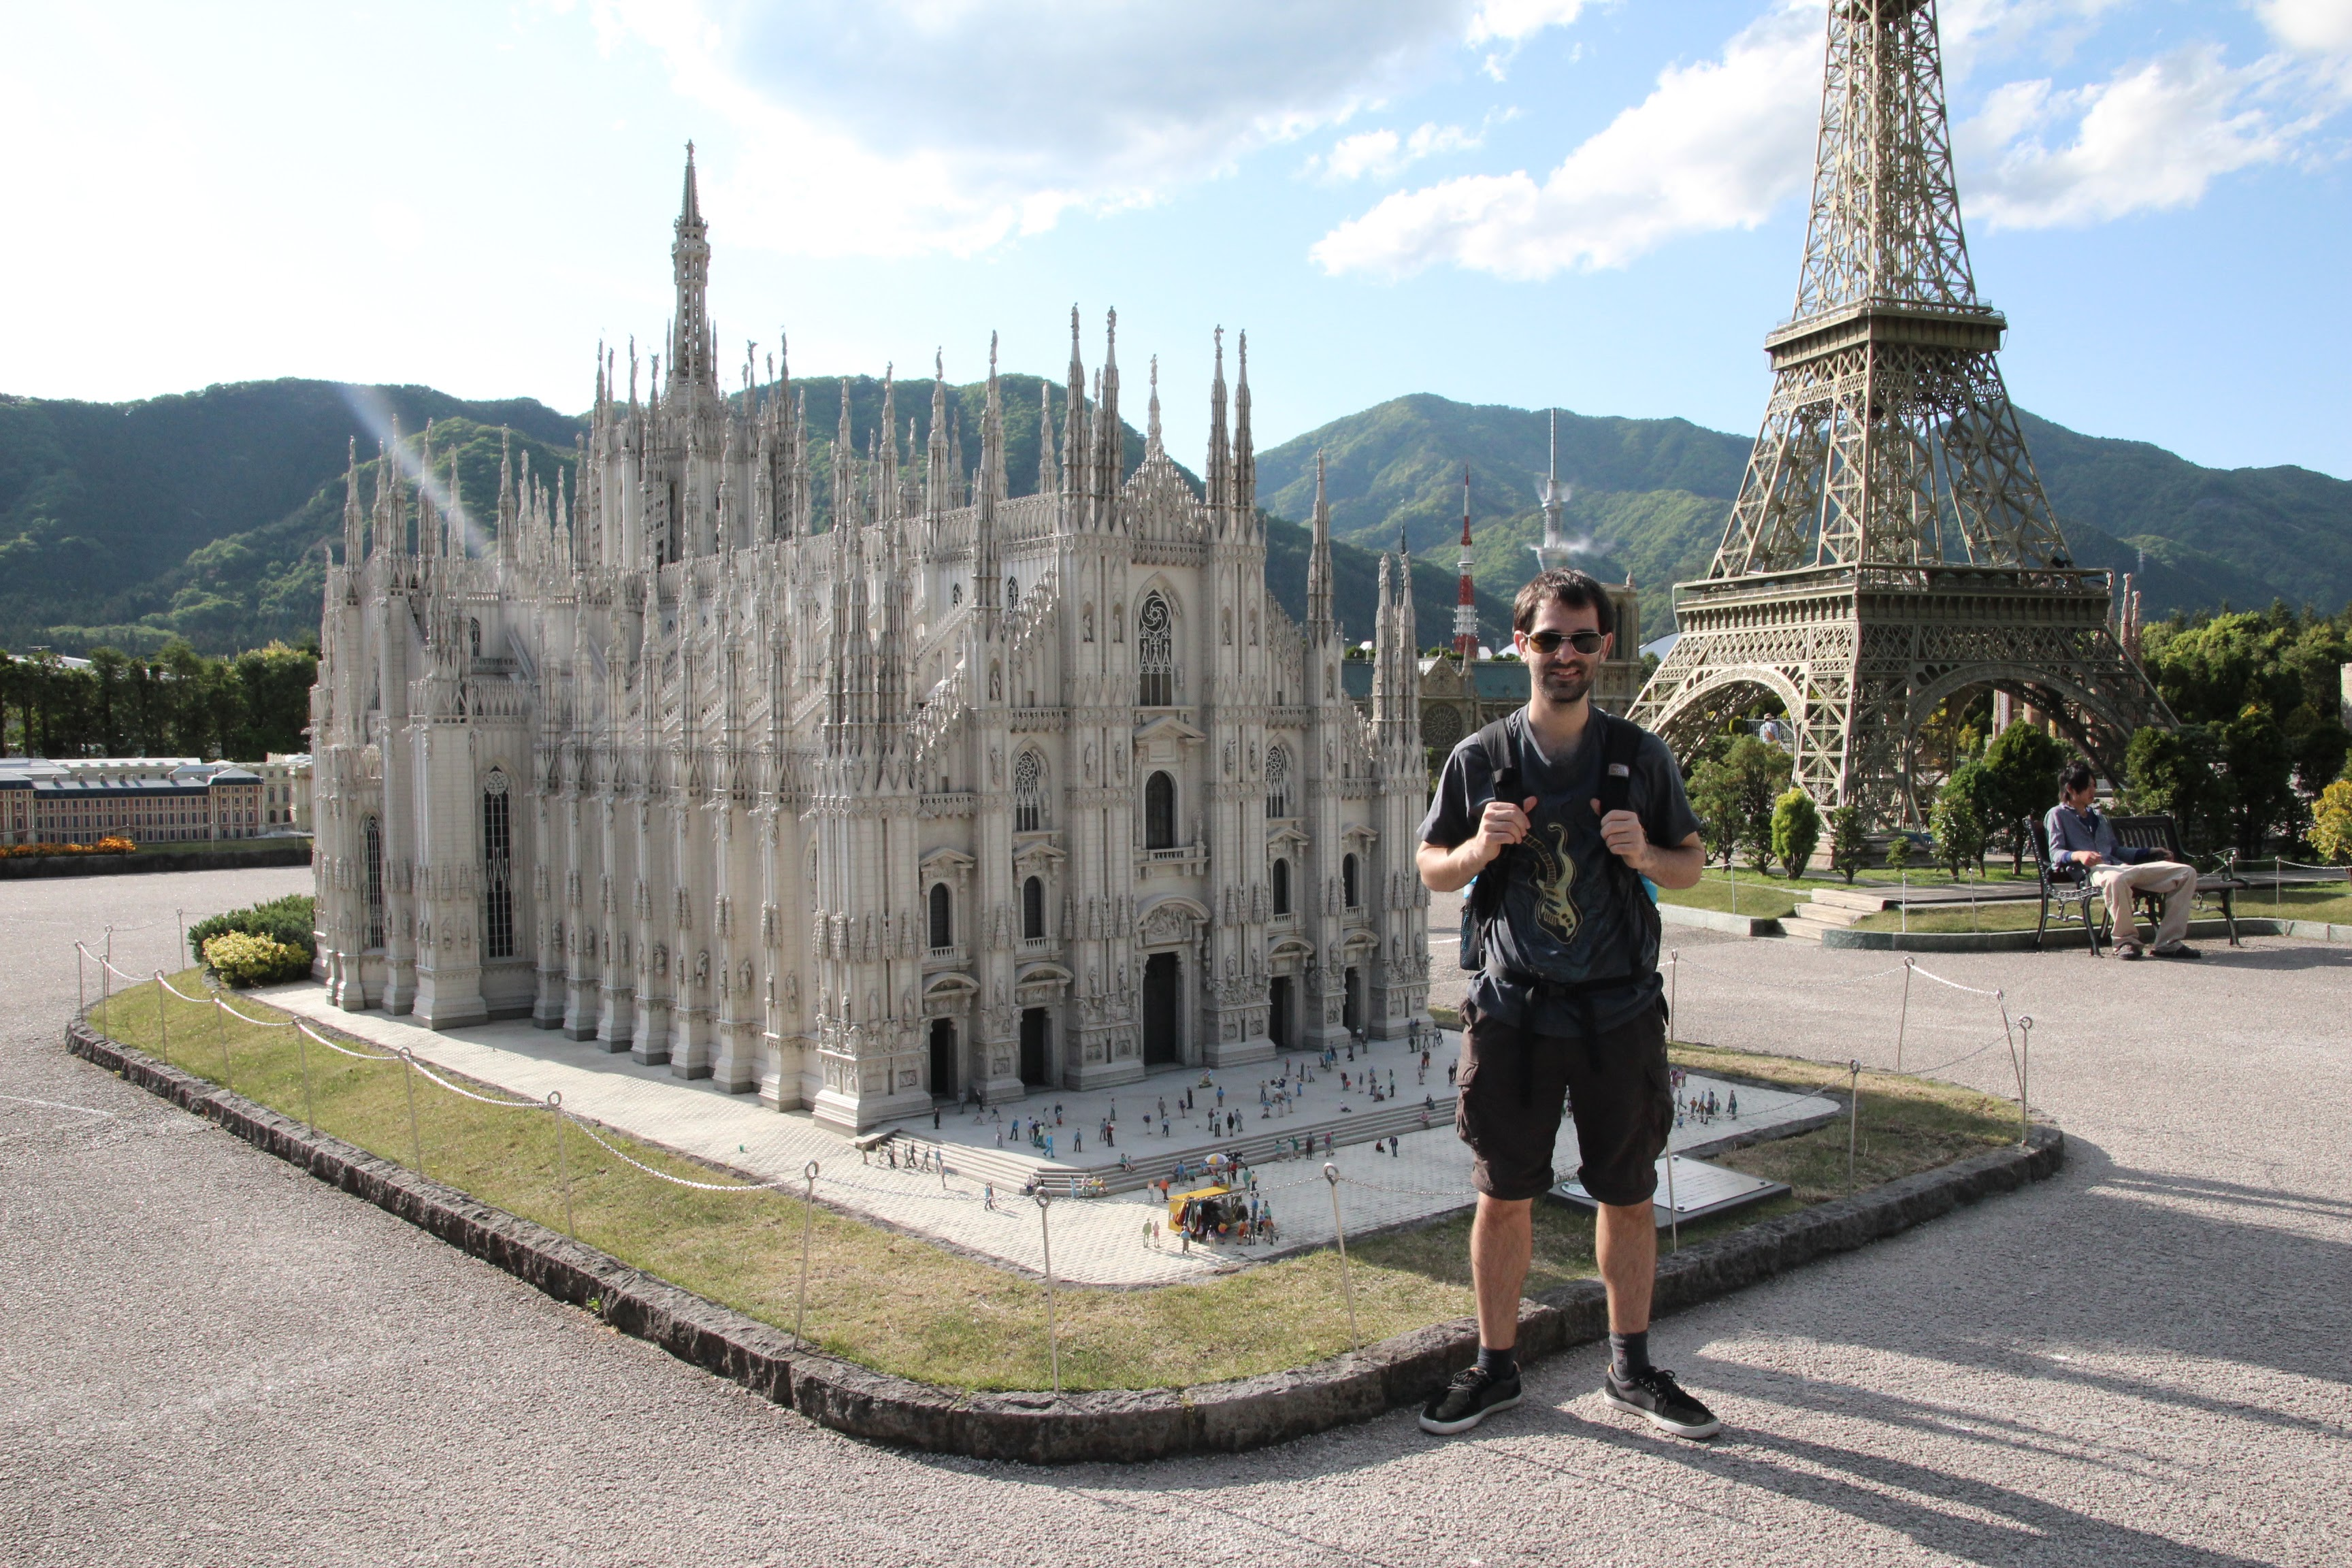
\includegraphics[width=\textwidth]{images/buildingScale.jpg}\end{center}
     \end{frame}
}


%% \begin{frame}{Absolute scale from visual measurements}
%%   How big is this building?
%%   \vspace{-2em}\begin{center}\includegraphics[width=\textwidth]{images/buildingDetour.png}\end{center}

%% \end{frame}

%% % we can tell the central door is bigger than the people
%% % but now way to determine physical quantities: how big, how far, how fast is the camera moving,..
%% % Even provided with many images
%% %

%% \begin{frame}{Absolute scale from visual measurements}
%%   \vspace{-2em}\begin{center}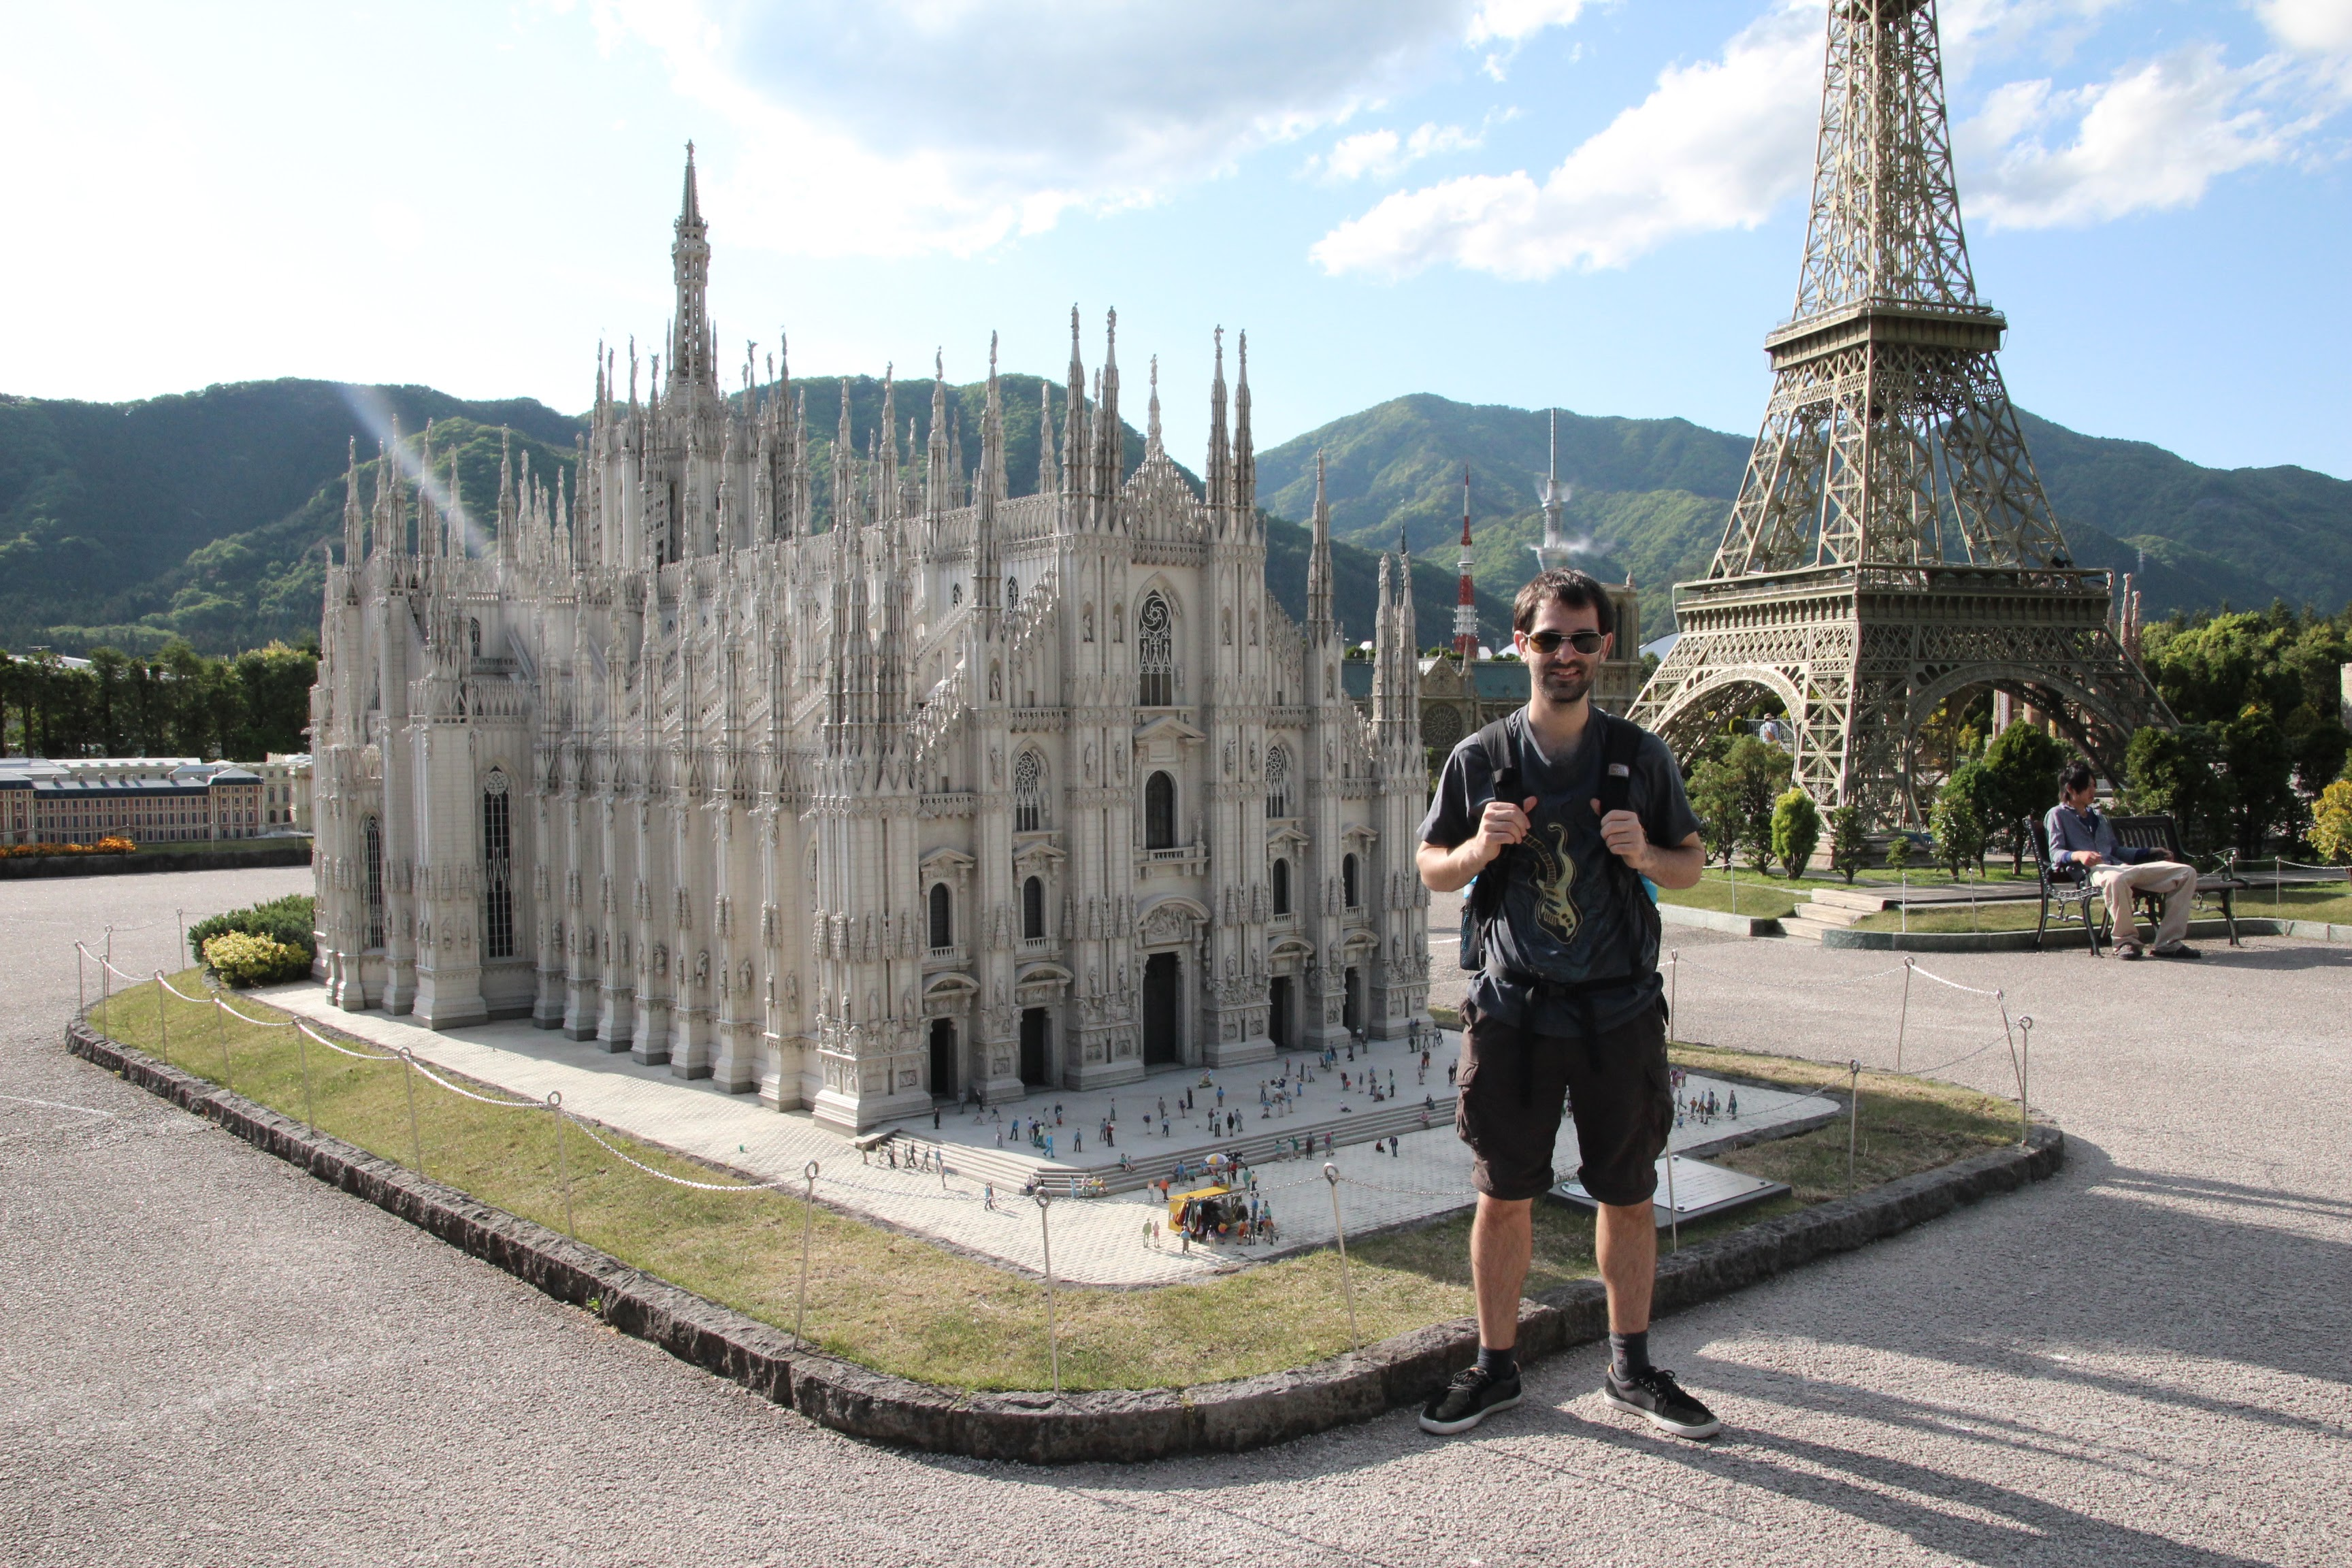
\includegraphics[width=\textwidth]{images/buildingScale.jpg}\end{center}
%% \end{frame}
%% % We need to known a physical quantity to set the absolute scale
%% % That's how drones are initialized..


\begin{frame}{Methods to recover the absolute scale}

  \begin{figure}
    \centering
    \begin{subfigure}[b]{0.3\textwidth}
      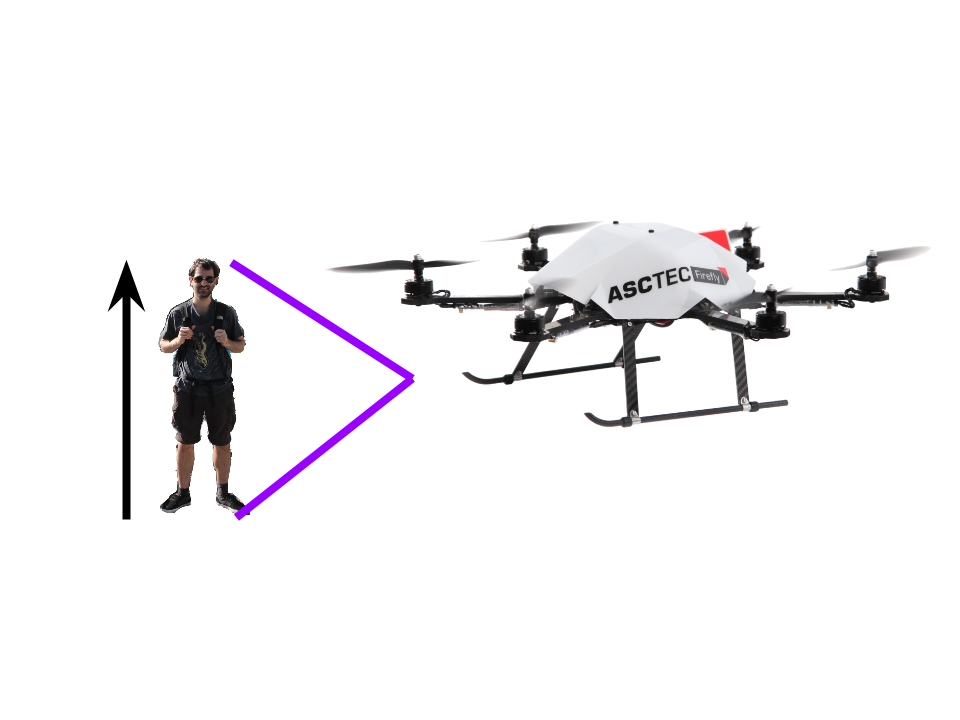
\includegraphics[width=\textwidth]{images/referenceInEnv.png}
      \onslide<4->{
        \caption{Not suited to unknown environments}
      }
    \end{subfigure}
    \onslide<2->{
      \begin{subfigure}[b]{0.3\textwidth}
        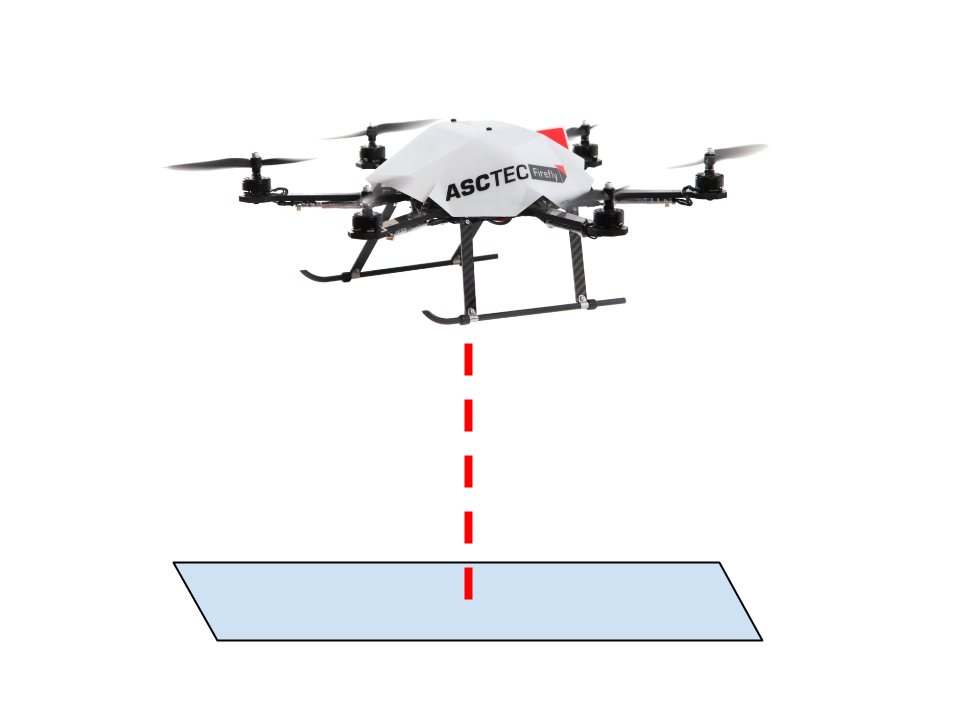
\includegraphics[width=\textwidth]{images/altitudeSensor.png}
      \onslide<4->{
        \caption{Not precise, works only in hover}
      }
      \end{subfigure}
    }
    \onslide<3->{
      \begin{subfigure}[b]{0.3\textwidth}
        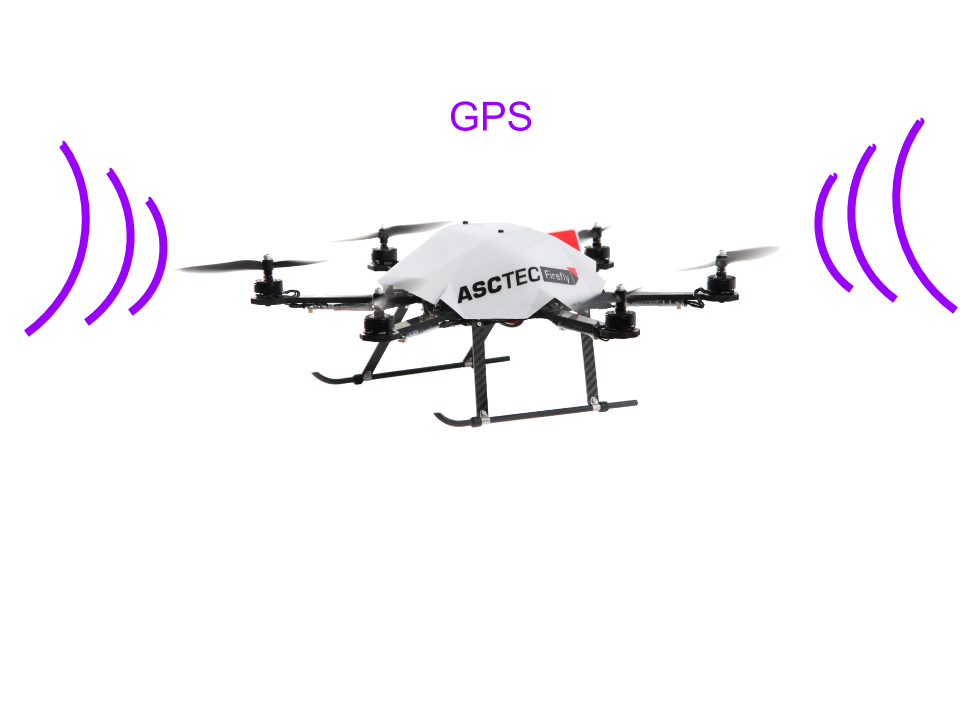
\includegraphics[width=\textwidth]{images/gpsSensor.png}
      \onslide<4->{
        \caption{Does not work in GPS denied environments}
      }
      \end{subfigure}
    }
  \end{figure}
\end{frame}

% so far we only considered visual measurements
% the IMU provides physical quantity (m/s^2 and rad/s)
\begin{frame}{Inertial Measurement Unit (IMU)}

The IMU consists of two sensors providing \textbf{physical quantities}:
\begin{itemize}
\item Accelerometer: linear acceleration (and gravity) ($m/s^2$);
\item Gyroscope: angular velocity ($rad/s$).
\end{itemize}

\end{frame}

\begin{frame}{Back to the title}
  \textcolor<4->{green}{Absolute scale velocity} \textcolor<3->{pink}{determination} combining \textcolor<2->{yellow}{visual and inertial measurements} for micro aerial vehicles

  \vspace{1em}


  \onslide<2->


  {\centering
    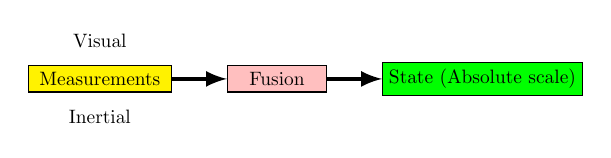
\begin{tikzpicture}[scale=\scalefilter, every node/.style={transform shape}]
      \node (A) [input, fill=yellow] {Measurements};
      \node (B) [above=2mm of A] {Visual};
      \node (C) [below=2mm of A] {Inertial};
      \node<3-> (D) [method,right=of A] {Fusion};
      \node<4-> (E) [input, right=of D, fill=\nodestatecolor] {State (Absolute scale)};
      \draw<3->[arr] (A.east) -- (D.west);
      \draw<4->[arr] (D.east) -- (E.west);
    \end{tikzpicture}
  }

\end{frame}
% \begin{frame}{Dead reckoning}
% Provided only with inertial measurements, we are subject to drift.

% %bias ?
% \end{frame}

\begin{frame}
\frametitle{Table of Contents}
\tableofcontents
\end{frame}

\section{The closed-form solution}

% So far, knowledge of previous state was required. Now we have a Closed-form solution that only relies on measurements over a short interval of time
\begin{frame}{The Closed-Form Solution - 2014}

Requires:
\begin{itemize}
\item Calibrated camera;
\item Inertial Measurement Unit (IMU);
\item External Camera IMU transformation.
\end{itemize}

Output:
\begin{itemize}
\item \textcolor<3->{red}{Initial velocity};
\item \textcolor<3->{green}{Distance to point-features};
\item \textcolor<3->{blue}{Attitude}.
\end{itemize}

\onslide<2->

\[
S_j = \textcolor<3->{green}{\lambda_1^i}\mu_1^i - \textcolor<3->{red}{V} t_j - \textcolor<3->{blue}{G} \frac{t_j^2}{2} - \textcolor<3->{green}{\lambda^i_j} \mu^i_j
\]
\end{frame}

\subsection{Linear system}
\begin{frame}{The Overconstrained Linear System}

  \[
  \textcolor<3->{green}{S_j} = \textcolor<3->{red}{\lambda_1^i}\textcolor<3->{blue}{\mu_1^i} - \textcolor<3->{red}{V}\textcolor<3->{blue}{t_j} - \textcolor<3->{red}{G} \textcolor<3->{blue}{\frac{t_j^2}{2}} - \textcolor<3->{red}{\lambda^i_j}\textcolor<3->{blue}{\mu^i_j}
  \]

  Valid for every point-feature $i$ at any time $t_j$:

  \onslide<2->
  \[
  \left[
    \begin{array}{c}
      \textcolor<3->{green}{S_2} = \textcolor<3->{red}{\lambda_1^1}\textcolor<3->{blue}{\mu_1^1} - \textcolor<3->{red}{V}\textcolor<3->{blue}{t_2} - \textcolor<3->{red}{G} \textcolor<3->{blue}{\frac{t_2^2}{2}} - \textcolor<3->{red}{\lambda^1_2}\textcolor<3->{blue}{\mu^1_2} \\
      \textcolor<3->{green}{S_2} = \textcolor<3->{red}{\lambda_1^2}\textcolor<3->{blue}{\mu_1^2} - \textcolor<3->{red}{V}\textcolor<3->{blue}{t_2} - \textcolor<3->{red}{G} \textcolor<3->{blue}{\frac{t_2^2}{2}} - \textcolor<3->{red}{\lambda^2_2}\textcolor<3->{blue}{\mu^2_2} \\
      \vdots \\
      \textcolor<3->{green}{S_3} = \textcolor<3->{red}{\lambda_1^1}\textcolor<3->{blue}{\mu_1^1} - \textcolor<3->{red}{V}\textcolor<3->{blue}{t_3} - \textcolor<3->{red}{G} \textcolor<3->{blue}{\frac{t_3^2}{2}} - \textcolor<3->{red}{\lambda^1_3}\textcolor<3->{blue}{\mu^1_3} \\
      \vdots \\
      \textcolor<3->{green}{S_N} = \textcolor<3->{red}{\lambda_1^{n_i}}\textcolor<3->{blue}{\mu_1^{n_i}} - \textcolor<3->{red}{V}\textcolor<3->{blue}{t_N} - \textcolor<3->{red}{G} \textcolor<3->{blue}{\frac{t_N^2}{2}} - \textcolor<3->{red}{\lambda^{n_i}_N}\textcolor<3->{blue}{\mu^{n_i}_N}
    \end{array}
    \right.
    \]

    \onslide<3->
    \[
    \textcolor{blue}{\Xi} \textcolor{red}{X} = \textcolor{green}{S}
    \]

\end{frame}


\begin{frame}{Problem: not robust in practice}
\emph{''\textbf{A closed-form solution} for state estimation with a visual-inertial system that does not require initialization was presented. However, this approach is \textbf{not suitable for systems that rely on noisy sensor data}''}\\
\rightline{{\rm --- Matthias Faessler, ICRA 2015}}

\begin{columns}
  \column<2->{.5\textwidth}
\begin{figure}[h!]
  \centering
  \resizebox{\textwidth}{!}{% This file was created by matlab2tikz.
% Minimal pgfplots version: 1.3
%
%The latest updates can be retrieved from
%  http://www.mathworks.com/matlabcentral/fileexchange/22022-matlab2tikz
%where you can also make suggestions and rate matlab2tikz.
%
\definecolor{mycolor1}{rgb}{0,1,0}%
%
\begin{tikzpicture}

\begin{axis}[%
width=4.5in,
height=3.7in,
at={(1.751579in,1.09421in)},
scale only axis,
xmin=1.5,
xmax=4.5,
xlabel={Duration (s)},
ymin=0,
ymax=1,
ylabel={Error},
xtick={1.5,2,...,4,4.5},
ytick={0.1,0.2,...,1,1.1},
legend style={legend cell align=left,align=left,draw=white!15!black}
]
\addlegendimage{line legend,blue} % or mark=none?
\addlegendentry{Lambda}
\addlegendimage{line legend,red}
\addlegendentry{Speed}
\addlegendimage{line legend,color=mycolor1}
\addlegendentry{Gravity}
\addplot [color=blue,solid]
  table[row sep=crcr]{%
1.5	0.762801178696159\\
2	0.490854841841618\\
2.5	0.460758656914928\\
3	0.481813646472708\\
3.5	0.461642438720163\\
4	0.437968480311408\\
4.5	0.409852108955419\\
};

\addplot [color=red,solid,forget plot]
  table[row sep=crcr]{%
1.5	0.897783065827637\\
2	0.625026337752138\\
2.5	0.594488594286172\\
3	0.625761539018411\\
3.5	0.555488396593806\\
4	0.465559666180634\\
4.5	0.362061397104667\\
};
\addplot [color=mycolor1,solid,forget plot]
  table[row sep=crcr]{%
1.5	0.152942570020578\\
2	0.0888439460940633\\
2.5	0.0761934019897938\\
3	0.069897164835093\\
3.5	0.0546837789020217\\
4	0.0447432430773695\\
4.5	0.0350875815151695\\
};

\end{axis}
\end{tikzpicture}%
}
\end{figure}
\column<3->{.5\textwidth}
$50\%$ relative error on speed and distance estimation
\end{columns}
\end{frame}

\begin{frame}{Improving the performance}
  What makes the estimations so bad?

  \begin{block}{Possible bottlenecks}
    \begin{itemize}
    \item<1-> Motion;
    \item<2-> Observed features;
    \item<3-> Noisy sensors.
    %%   \begin{itemize}
    %%   \item Impact of \textcolor{blue}{bias} on performance;
    %%   \item Impact of \textcolor{green}{non systematic errors} on performance.
    %%   \end{itemize}
    \end{itemize}
  \end{block}

  \onslide<4->
  Sensors provide measurements affected by a Gaussian noise:

  \[
  N(\mu + \textcolor<2->{blue}{B}, \textcolor<2->{green}{\sigma^2})
  \]

  \onslide<5->
  We considered:
  \begin{itemize}
  \item \textcolor{blue}{Biased} accelerometer;
  \item \textcolor{blue}{Biased} gyroscope.
  \end{itemize}
\end{frame}


%% \begin{frame}{Numerical stability}
%%   \[
%%   \left[
%%     \begin{array}{lcl}
%%       S_j &=& \lambda_1^i\mu_1^i - V t_j - G \frac{t_j^2}{2} - \lambda^i_j \mu^i_j\\
%%       0_3 &=& \lambda_1^1\mu_1^1 - \lambda_j^1\mu_j^1 - \lambda_1^i\mu_1^i + \lambda^i_j \mu^i_j
%%     \end{array}
%%   \right.
%%   \]

%% \[
%% S_j = \lambda_1^i\mu_1^i - V t_j - G \frac{t_j^2}{2} - \lambda^i_j \mu^i_j
%% \]
%% \end{frame}
\subsection{Identifying performance bottlenecks}
\begin{frame}{Biased inertial measurements}

  \begin{center}
    \textbf{Speed estimation error}
  \end{center}

  \begin{columns}[T]
    \column{.5\textwidth}
    \begin{figure}[h!]
      \centering
      \resizebox{0.85\textwidth}{!}{% This file was created by matlab2tikz.
% Minimal pgfplots version: 1.3
%
%The latest updates can be retrieved from
%  http://www.mathworks.com/matlabcentral/fileexchange/22022-matlab2tikz
%where you can also make suggestions and rate matlab2tikz.
%
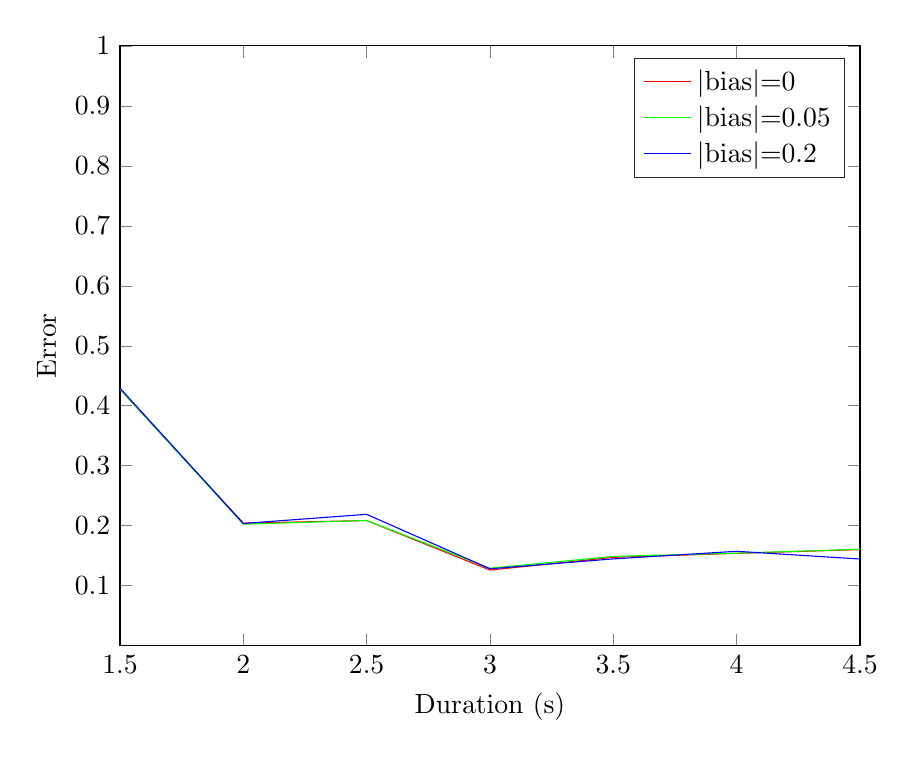
\begin{tikzpicture}

\begin{axis}[%
width=3.7in,
height=3in,
at={(1.751579in,1.09421in)},
scale only axis,
xmin=1.5,
xmax=4.5,
xlabel={ Duration (s)},
ytick={0.1,0.2,...,1,1.1},
xtick={1.5,2,...,4,4.5},
ymin=0,
ymax=1,
ylabel={Error},
title style={font=\bfseries},
legend style={legend cell align=left,align=left,draw=white!15!black}
]
\addplot [color=red,solid]
  table[row sep=crcr]{%
1.5	0.427463972747558\\
2	0.204392897471152\\
2.5	0.2086891919016\\
3	0.126226810629669\\
3.5	0.147352344834344\\
4	0.153986273651178\\
4.5	0.160248218913411\\
};
\addlegendentry{\textbar bias\textbar=0};

\addplot [color=green,solid]
  table[row sep=crcr]{%
1.5	0.427842146458304\\
2	0.20268073059906\\
2.5	0.208771544411042\\
3	0.129271147402759\\
3.5	0.148897086867292\\
4	0.154358837863052\\
4.5	0.16081022719229\\
};
\addlegendentry{\textbar bias\textbar =0.05};

\addplot [color=blue,solid]
  table[row sep=crcr]
      \caption{Varying accelerometer bias}
    \end{figure}
    \column{.5\textwidth}
    \begin{figure}[h!]
      \centering
      \resizebox{0.85\textwidth}{!}{% This file was created by matlab2tikz.
% Minimal pgfplots version: 1.3
%
%The latest updates can be retrieved from
%  http://www.mathworks.com/matlabcentral/fileexchange/22022-matlab2tikz
%where you can also make suggestions and rate matlab2tikz.
%
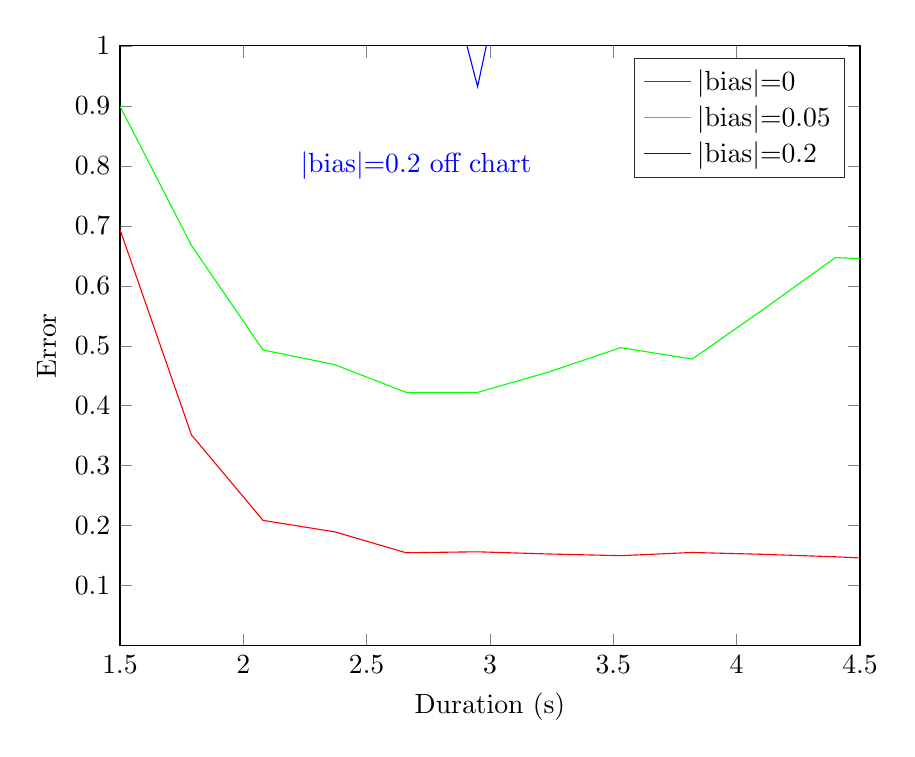
\begin{tikzpicture}

\begin{axis}[%
width=3.7in,
height=3in,
at={(1.751579in,1.09421in)},
scale only axis,
unbounded coords=jump,
xmin=1.5,
xmax=4.5,
xlabel={Duration (s)},
ytick={0.1,0.2,...,1,1.1},
xtick={1.5,2,...,4,4.5},
ymin=0,
ymax=1,
ylabel={Error },
title style={font=\bfseries},
legend style={legend cell align=left,align=left,draw=white!15!black}
]
\addplot [color=red,solid]
  table[row sep=crcr]{%
1.5	0.69385799743164\\
1.79	0.351400106646042\\
2.08	0.208972359940106\\
2.37	0.189904693757416\\
2.66	0.155031673380865\\
2.95	0.156603969287685\\
3.24	0.152939916596076\\
3.53	0.150155750111395\\
3.82	0.15549617974511\\
4.11	0.152358693836919\\
4.4	0.148302651272463\\
4.69	0.142615204897316\\
};
\addlegendentry{\textbar bias\textbar =0};

\addplot [color=green,solid]
  table[row sep=crcr]{%
1.5	0.899343688689263\\
1.79	0.6670895311607\\
2.08	0.492994031916181\\
2.37	0.468605658830025\\
2.66	0.422315774521047\\
2.95	0.422348108072392\\
3.24	0.456442867280175\\
3.53	0.496882747914263\\
3.82	0.477797052531491\\
4.11	0.561139746296675\\
4.4	0.646949430497149\\
4.69	0.642082595006945\\
};
\addlegendentry{\textbar bias\textbar =0.05};

\addplot [color=blue,solid]
  table[row sep=crcr]
      \caption{Varying gyroscope bias}
    \end{figure}

  \end{columns}
\end{frame}

\subsection{Estimating the gyroscope bias}
\begin{frame}{Estimating the gyroscope bias}

  \begin{itemize}[<+->]
  \item When solving  $\Xi X = S$, we are solving $\argmin_X ||\Xi X - S||^2$;
  \item Unfortunately, we can not express the gyroscope bias linearly;
  \item Alternative: non-linear minimization
  \[
  \argmin_{\textcolor{red}{B},X} ||\Xi X - S||^2 \onslide<5->{\textcolor{blue}{+ \lambda \times |B|}}
  \]
  {\tiny With $B$ the gyroscope bias, $\Xi$ and $S$ computed with respect to $B$}
  \end{itemize}

  \onslide<4->
  \begin{figure}[h!]
    \centering
      \begin{subfigure}[b]{0.47\textwidth}
        \resizebox{\textwidth}{!}{% This file was created by matlab2tikz.
% Minimal pgfplots version: 1.3
%
%The latest updates can be retrieved from
%  http://www.mathworks.com/matlabcentral/fileexchange/22022-matlab2tikz
%where you can also make suggestions and rate matlab2tikz.
%
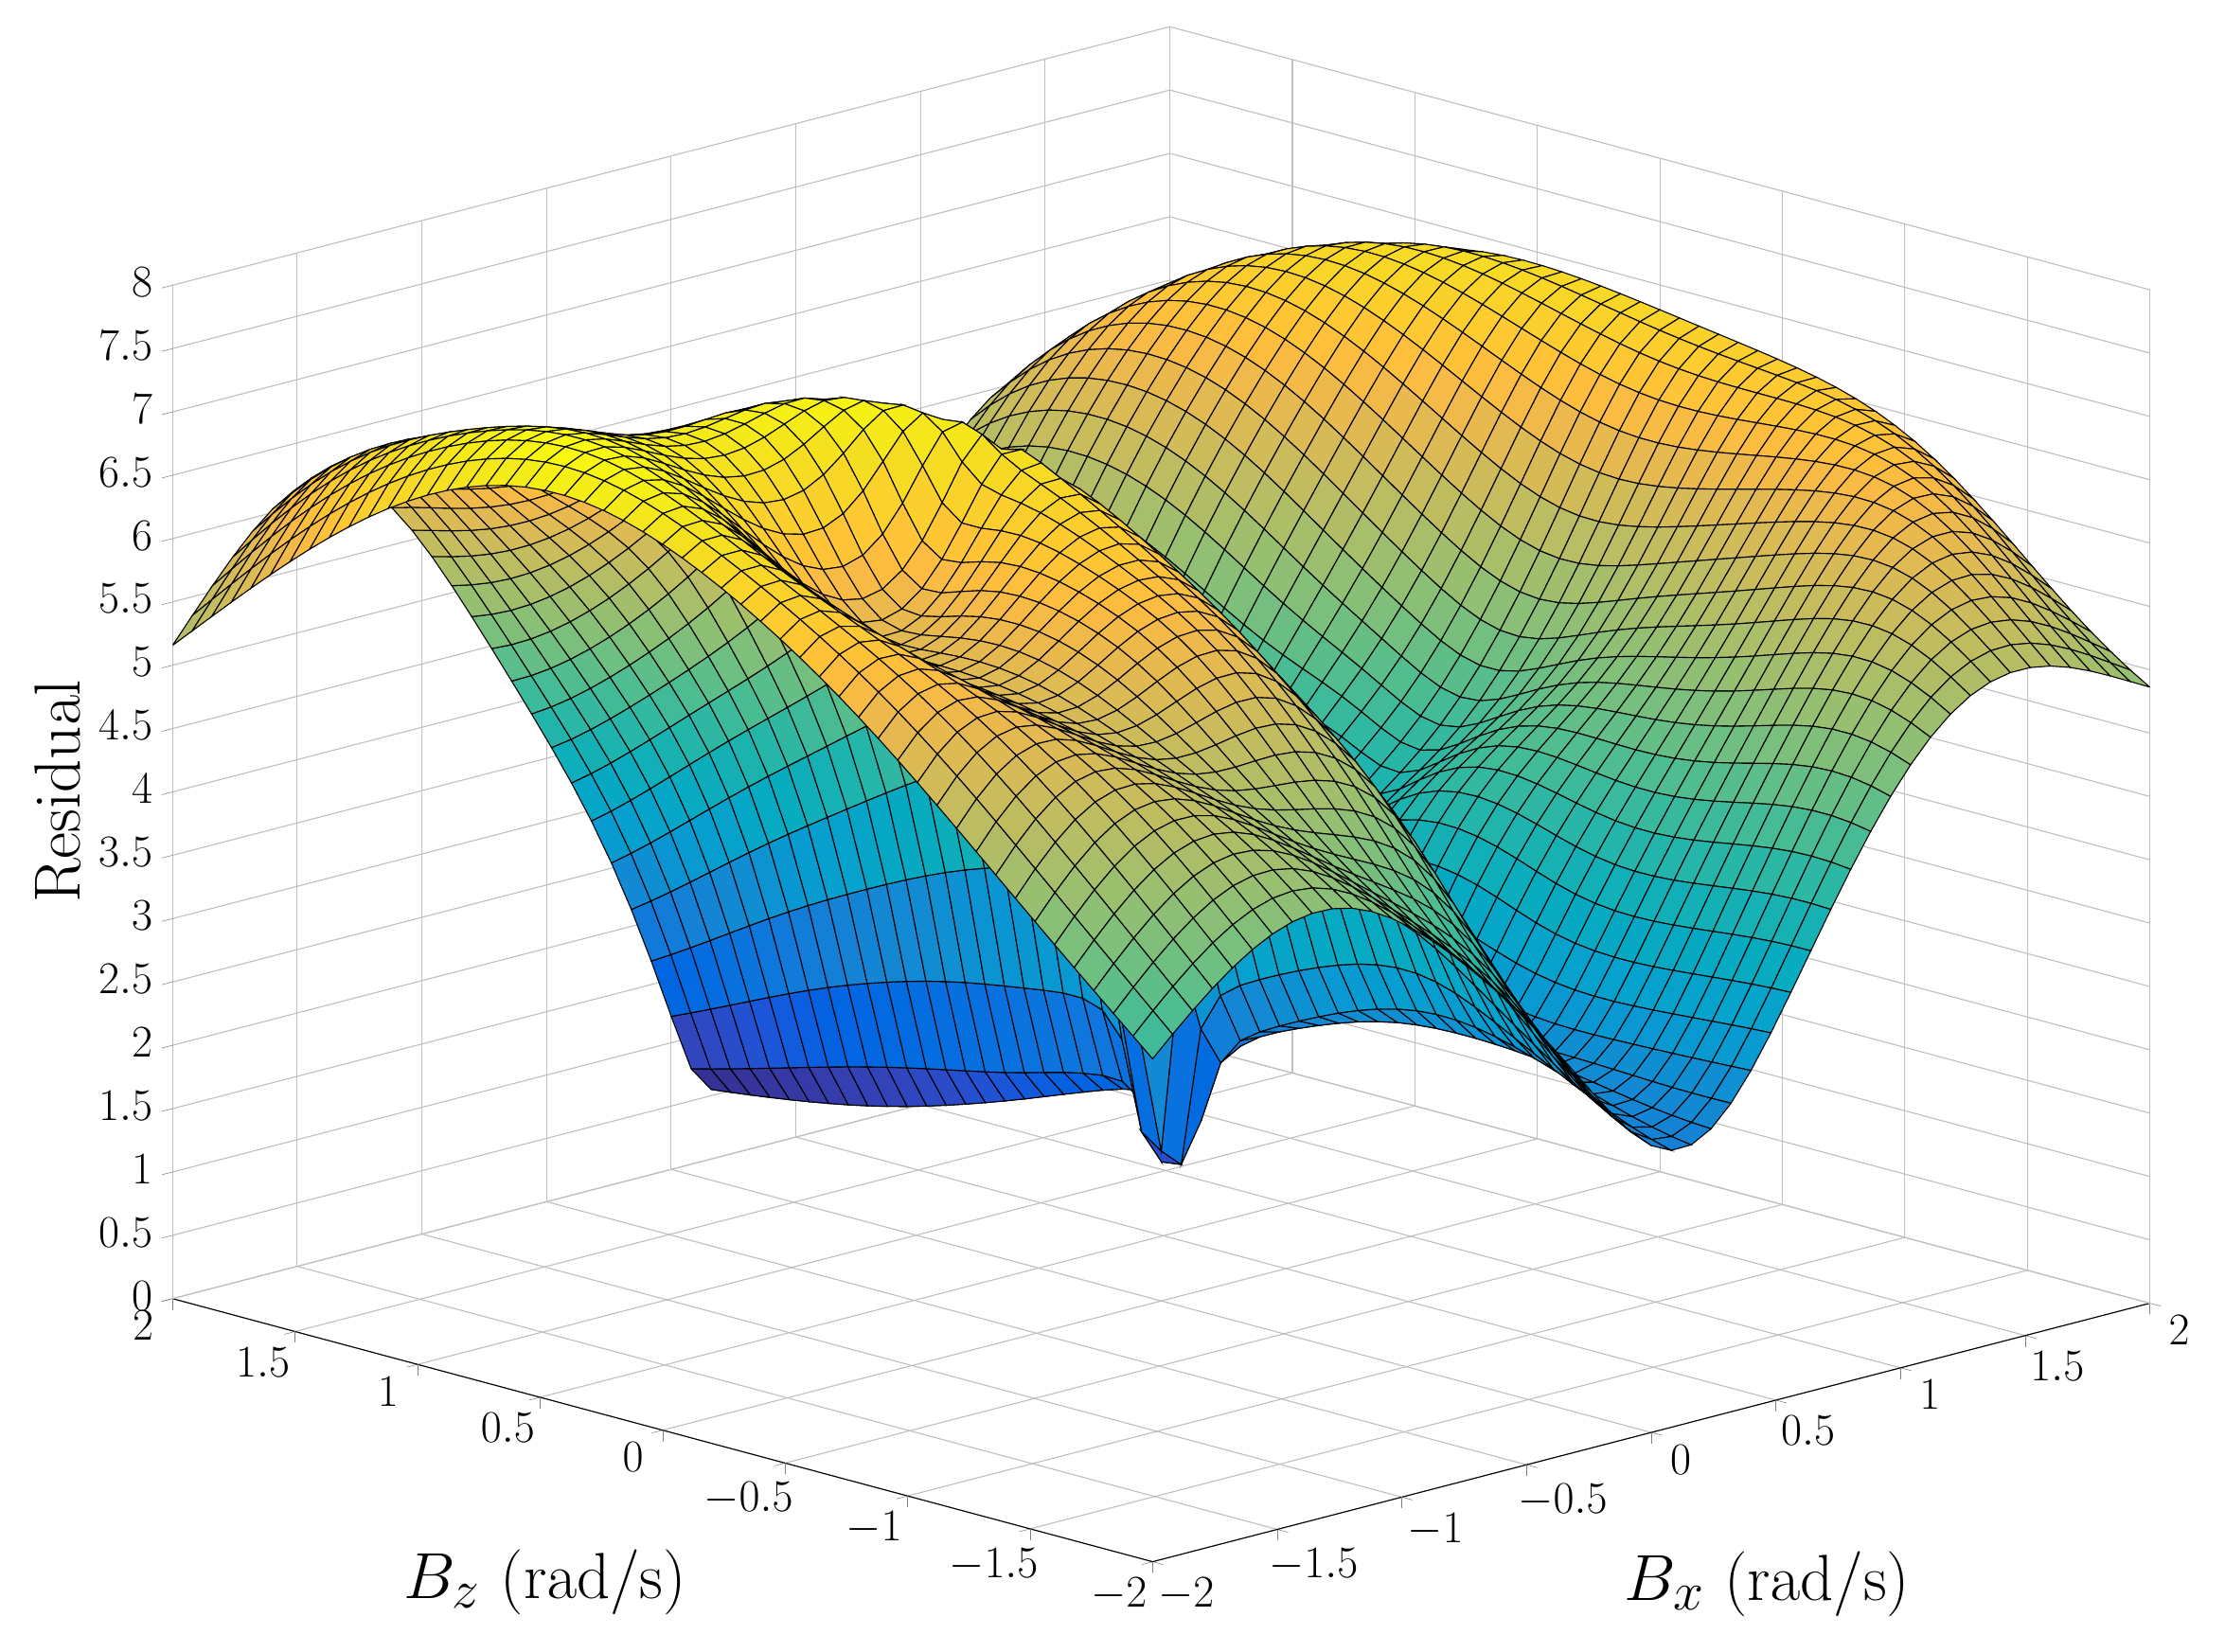
\begin{tikzpicture}

\begin{axis}[%
width=10.442105in,
height=8.107105in,
at={(0.921556in,1.181889in)},
scale only axis,
xmin=-2,
xmax=2,
tick align=outside,
xlabel={\Huge $B_x$ (rad/s)},
xmajorgrids,
ymin=-2,
ymax=2,
xtick={-2,-1.5,...,1.5,2},
ytick={-2,-1.5,...,1.5,2},
ticklabel style = {font=\LARGE},
ylabel={\Huge $B_z$ (rad/s)},
zlabel={\Huge Residual},
ymajorgrids,
zmin=0,
zmax=8,
zmajorgrids,
view={-44.5}{20},
axis x line*=bottom,
axis y line*=left,
axis z line*=left
]

\addplot3[%
surf,
faceted color=black,
shader=faceted,
colormap={mymap}{[1pt] rgb(0pt)=(0.2081,0.1663,0.5292); rgb(1pt)=(0.211624,0.189781,0.577676); rgb(2pt)=(0.212252,0.213771,0.626971); rgb(3pt)=(0.2081,0.2386,0.677086); rgb(4pt)=(0.195905,0.264457,0.7279); rgb(5pt)=(0.170729,0.291938,0.779248); rgb(6pt)=(0.125271,0.324243,0.830271); rgb(7pt)=(0.0591333,0.359833,0.868333); rgb(8pt)=(0.0116952,0.38751,0.881957); rgb(9pt)=(0.00595714,0.408614,0.882843); rgb(10pt)=(0.0165143,0.4266,0.878633); rgb(11pt)=(0.0328524,0.443043,0.871957); rgb(12pt)=(0.0498143,0.458571,0.864057); rgb(13pt)=(0.0629333,0.47369,0.855438); rgb(14pt)=(0.0722667,0.488667,0.8467); rgb(15pt)=(0.0779429,0.503986,0.838371); rgb(16pt)=(0.0793476,0.520024,0.831181); rgb(17pt)=(0.0749429,0.537543,0.826271); rgb(18pt)=(0.0640571,0.556986,0.823957); rgb(19pt)=(0.0487714,0.577224,0.822829); rgb(20pt)=(0.0343429,0.596581,0.819852); rgb(21pt)=(0.0265,0.6137,0.8135); rgb(22pt)=(0.0238905,0.628662,0.803762); rgb(23pt)=(0.0230905,0.641786,0.791267); rgb(24pt)=(0.0227714,0.653486,0.776757); rgb(25pt)=(0.0266619,0.664195,0.760719); rgb(26pt)=(0.0383714,0.674271,0.743552); rgb(27pt)=(0.0589714,0.683757,0.725386); rgb(28pt)=(0.0843,0.692833,0.706167); rgb(29pt)=(0.113295,0.7015,0.685857); rgb(30pt)=(0.145271,0.709757,0.664629); rgb(31pt)=(0.180133,0.717657,0.642433); rgb(32pt)=(0.217829,0.725043,0.619262); rgb(33pt)=(0.258643,0.731714,0.595429); rgb(34pt)=(0.302171,0.737605,0.571186); rgb(35pt)=(0.348167,0.742433,0.547267); rgb(36pt)=(0.395257,0.7459,0.524443); rgb(37pt)=(0.44201,0.748081,0.503314); rgb(38pt)=(0.487124,0.749062,0.483976); rgb(39pt)=(0.530029,0.749114,0.466114); rgb(40pt)=(0.570857,0.748519,0.44939); rgb(41pt)=(0.609852,0.747314,0.433686); rgb(42pt)=(0.6473,0.7456,0.4188); rgb(43pt)=(0.683419,0.743476,0.404433); rgb(44pt)=(0.71841,0.741133,0.390476); rgb(45pt)=(0.752486,0.7384,0.376814); rgb(46pt)=(0.785843,0.735567,0.363271); rgb(47pt)=(0.818505,0.732733,0.34979); rgb(48pt)=(0.850657,0.7299,0.336029); rgb(49pt)=(0.882433,0.727433,0.3217); rgb(50pt)=(0.913933,0.725786,0.306276); rgb(51pt)=(0.944957,0.726114,0.288643); rgb(52pt)=(0.973895,0.731395,0.266648); rgb(53pt)=(0.993771,0.745457,0.240348); rgb(54pt)=(0.999043,0.765314,0.216414); rgb(55pt)=(0.995533,0.786057,0.196652); rgb(56pt)=(0.988,0.8066,0.179367); rgb(57pt)=(0.978857,0.827143,0.163314); rgb(58pt)=(0.9697,0.848138,0.147452); rgb(59pt)=(0.962586,0.870514,0.1309); rgb(60pt)=(0.958871,0.8949,0.113243); rgb(61pt)=(0.959824,0.921833,0.0948381); rgb(62pt)=(0.9661,0.951443,0.0755333); rgb(63pt)=(0.9763,0.9831,0.0538)},
mesh/rows=51]
table[row sep=crcr,header=false] {%
%
-2	-2	3.96953559596561\\
-2	-1.92	4.10768647002591\\
-2	-1.84	4.24569847297076\\
-2	-1.76	4.3840218213466\\
-2	-1.68	4.52305616147229\\
-2	-1.6	4.66307817919315\\
-2	-1.52	4.80418369276614\\
-2	-1.44	4.94625064166626\\
-2	-1.36	5.08892766050472\\
-2	-1.28	5.23165000647402\\
-2	-1.2	5.37368084411246\\
-2	-1.12	5.51417201162251\\
-2	-1.04	5.65223532899549\\
-2	-0.96	5.78701409946557\\
-2	-0.88	5.91774508904903\\
-2	-0.8	6.04380361330781\\
-2	-0.72	6.16472743291698\\
-2	-0.64	6.28021782446951\\
-2	-0.56	6.39011787978065\\
-2	-0.48	6.49436921231523\\
-2	-0.4	6.59294989381992\\
-2	-0.32	6.68579940086098\\
-2	-0.24	6.77274030366729\\
-2	-0.16	6.85340998046518\\
-2	-0.0800000000000001	6.92721707426617\\
-2	0	6.99333544574209\\
-2	0.0800000000000001	7.05074252721512\\
-2	0.16	7.09829983478544\\
-2	0.24	7.13486298666621\\
-2	0.32	7.15940026194346\\
-2	0.4	7.17109590087901\\
-2	0.48	7.16941848756345\\
-2	0.56	7.15414442647747\\
-2	0.64	7.12533813500834\\
-2	0.72	7.08330030278077\\
-2	0.8	7.02850093029741\\
-2	0.88	6.96151416647848\\
-2	0.96	6.88296800946441\\
-2	1.04	6.79351545772275\\
-2	1.12	6.69382684182674\\
-2	1.2	6.58459778282305\\
-2	1.28	6.46656469268609\\
-2	1.36	6.34052002784537\\
-2	1.44	6.20732170347499\\
-2	1.52	6.06789381913412\\
-2	1.6	5.9232180635586\\
-2	1.68	5.77431649081623\\
-2	1.76	5.62222704624045\\
-2	1.84	5.46797373702601\\
-2	1.92	5.31253397981478\\
-2	2	5.15680635884562\\
-1.92	-2	4.12256554777728\\
-1.92	-1.92	4.26668432204039\\
-1.92	-1.84	4.41087178326284\\
-1.92	-1.76	4.55542689958074\\
-1.92	-1.68	4.70052423361521\\
-1.92	-1.6	4.84615330214983\\
-1.92	-1.52	4.99207973536112\\
-1.92	-1.44	5.13783397629943\\
-1.92	-1.36	5.2827306352235\\
-1.92	-1.28	5.42591774877334\\
-1.92	-1.2	5.56645052138299\\
-1.92	-1.12	5.7033796130576\\
-1.92	-1.04	5.83584103863677\\
-1.92	-0.96	5.96313446784647\\
-1.92	-0.88	6.08477949096741\\
-1.92	-0.8	6.20054423823241\\
-1.92	-0.72	6.31044557436716\\
-1.92	-0.64	6.41472294711033\\
-1.92	-0.56	6.5137882238851\\
-1.92	-0.48	6.60815282316808\\
-1.92	-0.4	6.69833359986875\\
-1.92	-0.32	6.78474207655356\\
-1.92	-0.24	6.86756747660566\\
-1.92	-0.16	6.94667051861043\\
-1.92	-0.0800000000000001	7.02150941909083\\
-1.92	0	7.0911196745187\\
-1.92	0.0800000000000001	7.15416304991952\\
-1.92	0.16	7.20904800422466\\
-1.92	0.24	7.2541055973428\\
-1.92	0.32	7.28778763995639\\
-1.92	0.4	7.30884505616819\\
-1.92	0.48	7.31644880345962\\
-1.92	0.56	7.31023172356702\\
-1.92	0.64	7.29025081294116\\
-1.92	0.72	7.25688814385105\\
-1.92	0.8	7.21072011503312\\
-1.92	0.88	7.15238731759473\\
-1.92	0.96	7.08249211531543\\
-1.92	1.04	7.00154068237248\\
-1.92	1.12	6.90993401657131\\
-1.92	1.2	6.80800144816006\\
-1.92	1.28	6.6960625463911\\
-1.92	1.36	6.57449994876512\\
-1.92	1.44	6.4438261781428\\
-1.92	1.52	6.30473091971276\\
-1.92	1.6	6.15810030142864\\
-1.92	1.68	6.00500547663265\\
-1.92	1.76	5.84666343023339\\
-1.92	1.84	5.68437752083278\\
-1.92	1.92	5.51946793219248\\
-1.92	2	5.35320252672805\\
-1.84	-2	4.26817660315442\\
-1.84	-1.92	4.41756364181435\\
-1.84	-1.84	4.56692433772459\\
-1.84	-1.76	4.71628611412794\\
-1.84	-1.68	4.86548461712527\\
-1.84	-1.6	5.01412551775112\\
-1.84	-1.52	5.16157591177941\\
-1.84	-1.44	5.30698926125651\\
-1.84	-1.36	5.4493641076256\\
-1.84	-1.28	5.5876316473392\\
-1.84	-1.2	5.72076142350429\\
-1.84	-1.12	5.84786958026397\\
-1.84	-1.04	5.96831253042371\\
-1.84	-0.96	6.08175189141002\\
-1.84	-0.88	6.18818356533774\\
-1.84	-0.8	6.28793212190221\\
-1.84	-0.72	6.38161744791494\\
-1.84	-0.64	6.47010129010687\\
-1.84	-0.56	6.55441705352494\\
-1.84	-0.48	6.63568041865717\\
-1.84	-0.4	6.71497573179798\\
-1.84	-0.32	6.79321669562466\\
-1.84	-0.24	6.87098905305687\\
-1.84	-0.16	6.94839457713728\\
-1.84	-0.0800000000000001	7.02492631688921\\
-1.84	0	7.09941135021931\\
-1.84	0.0800000000000001	7.1700546492594\\
-1.84	0.16	7.2346010696438\\
-1.84	0.24	7.29060169056717\\
-1.84	0.32	7.33573531066088\\
-1.84	0.4	7.36811262527784\\
-1.84	0.48	7.38649242352188\\
-1.84	0.56	7.39036540846271\\
-1.84	0.64	7.37989910161782\\
-1.84	0.72	7.35577158108122\\
-1.84	0.8	7.31894303899675\\
-1.84	0.88	7.27041980958118\\
-1.84	0.96	7.21105787839203\\
-1.84	1.04	7.14143685320625\\
-1.84	1.12	7.06181672429096\\
-1.84	1.2	6.97217322641791\\
-1.84	1.28	6.87229572586919\\
-1.84	1.36	6.76192453410124\\
-1.84	1.44	6.64090143060214\\
-1.84	1.52	6.50930702267799\\
-1.84	1.6	6.36756123818174\\
-1.84	1.68	6.21646936578914\\
-1.84	1.76	6.05720606396812\\
-1.84	1.84	5.89124243832386\\
-1.84	1.92	5.72023316228771\\
-1.84	2	5.54588746760841\\
-1.76	-2	4.40328552747556\\
-1.76	-1.92	4.55670966374549\\
-1.76	-1.84	4.70956836166359\\
-1.76	-1.76	4.86150661116584\\
-1.76	-1.68	5.01193114339525\\
-1.76	-1.6	5.16000799368019\\
-1.76	-1.52	5.30469706382988\\
-1.76	-1.44	5.44482386110451\\
-1.76	-1.36	5.57918305009132\\
-1.76	-1.28	5.70666162048795\\
-1.76	-1.2	5.82636319868087\\
-1.76	-1.12	5.93771230323948\\
-1.76	-1.04	6.04052067465287\\
-1.76	-0.96	6.13500726588581\\
-1.76	-0.88	6.22177589121777\\
-1.76	-0.8	6.30176465415031\\
-1.76	-0.72	6.37618432216034\\
-1.76	-0.64	6.44645696895032\\
-1.76	-0.56	6.51415400079994\\
-1.76	-0.48	6.5809204388966\\
-1.76	-0.4	6.64836707175863\\
-1.76	-0.32	6.71791724518849\\
-1.76	-0.24	6.79060868127472\\
-1.76	-0.16	6.86686864946821\\
-1.76	-0.0800000000000001	6.94630065196898\\
-1.76	0	7.02754018327651\\
-1.76	0.0800000000000001	7.10824746702435\\
-1.76	0.16	7.18529071848165\\
-1.76	0.24	7.25512419637796\\
-1.76	0.32	7.31429391901961\\
-1.76	0.4	7.3599471292927\\
-1.76	0.48	7.39021384584179\\
-1.76	0.56	7.40437336681156\\
-1.76	0.64	7.40278797126489\\
-1.76	0.72	7.38664786417496\\
-1.76	0.8	7.35760776173661\\
-1.76	0.88	7.31740364183628\\
-1.76	0.96	7.2675236932963\\
-1.76	1.04	7.20898020494889\\
-1.76	1.12	7.14220010385522\\
-1.76	1.2	7.06702945291546\\
-1.76	1.28	6.98283432714661\\
-1.76	1.36	6.8886749061129\\
-1.76	1.44	6.78352690162109\\
-1.76	1.52	6.66652100673566\\
-1.76	1.6	6.53716629256946\\
-1.76	1.68	6.39552039526287\\
-1.76	1.76	6.24227325198951\\
-1.76	1.84	6.07872609892112\\
-1.76	1.92	5.90667171126118\\
-1.76	2	5.72820663959609\\
-1.68	-2	4.52442817444724\\
-1.68	-1.92	4.6800196488908\\
-1.68	-1.84	4.83395797726146\\
-1.68	-1.76	4.98542947430613\\
-1.68	-1.68	5.13337717696746\\
-1.68	-1.6	5.27654994518269\\
-1.68	-1.52	5.41359285621812\\
-1.68	-1.44	5.54317100012462\\
-1.68	-1.36	5.66411102282432\\
-1.68	-1.28	5.77553786095503\\
-1.68	-1.2	5.8769814409298\\
-1.68	-1.12	5.96843276499073\\
-1.68	-1.04	6.05034111884961\\
-1.68	-0.96	6.12356048389156\\
-1.68	-0.88	6.18926737189971\\
-1.68	-0.8	6.24887833552567\\
-1.68	-0.72	6.303990328886\\
-1.68	-0.64	6.35635180234238\\
-1.68	-0.56	6.40785192524329\\
-1.68	-0.48	6.46049798270151\\
-1.68	-0.4	6.51634492297579\\
-1.68	-0.32	6.57734855745127\\
-1.68	-0.24	6.64513029621805\\
-1.68	-0.16	6.72066221251066\\
-1.68	-0.0800000000000001	6.80391030942226\\
-1.68	0	6.89351649114508\\
-1.68	0.0800000000000001	6.98664419647848\\
-1.68	0.16	7.07912021833977\\
-1.68	0.24	7.16593429510817\\
-1.68	0.32	7.24201644126465\\
-1.68	0.4	7.30307877418483\\
-1.68	0.48	7.34627449764164\\
-1.68	0.56	7.37050799261757\\
-1.68	0.64	7.37636255036981\\
-1.68	0.72	7.36572298957398\\
-1.68	0.8	7.34122782555508\\
-1.68	0.88	7.30569250291519\\
-1.68	0.96	7.26161540018844\\
-1.68	1.04	7.21082966139778\\
-1.68	1.12	7.15431621098008\\
-1.68	1.2	7.09216157331658\\
-1.68	1.28	7.02363249018917\\
-1.68	1.36	6.94734204521142\\
-1.68	1.44	6.86148901478261\\
-1.68	1.52	6.76415436060813\\
-1.68	1.6	6.65363112862622\\
-1.68	1.68	6.52874765896951\\
-1.68	1.76	6.38912743892591\\
-1.68	1.84	6.23532585230776\\
-1.68	1.92	6.06880540637501\\
-1.68	2	5.8917542370859\\
-1.6	-2	4.62778433556879\\
-1.6	-1.92	4.78301319347452\\
-1.6	-1.84	4.93492304277036\\
-1.6	-1.76	5.0822352271011\\
-1.6	-1.68	5.22349124598085\\
-1.6	-1.6	5.35716776034462\\
-1.6	-1.52	5.48182661935434\\
-1.6	-1.44	5.59627747185312\\
-1.6	-1.36	5.69972370273108\\
-1.6	-1.28	5.79186192975515\\
-1.6	-1.2	5.87291363455427\\
-1.6	-1.12	5.94358395450792\\
-1.6	-1.04	6.00496239199529\\
-1.6	-0.96	6.05839621134074\\
-1.6	-0.88	6.10537405301387\\
-1.6	-0.8	6.14745292132042\\
-1.6	-0.72	6.1862472936714\\
-1.6	-0.64	6.22347725320662\\
-1.6	-0.56	6.26104803911255\\
-1.6	-0.48	6.30111459754974\\
-1.6	-0.4	6.3460798676179\\
-1.6	-0.32	6.39848413251494\\
-1.6	-0.24	6.46075466632553\\
-1.6	-0.16	6.53479631643089\\
-1.6	-0.0800000000000001	6.62143312995678\\
-1.6	0	6.71978784984478\\
-1.6	0.0800000000000001	6.82680587560688\\
-1.6	0.16	6.93721320640349\\
-1.6	0.24	7.04411840830546\\
-1.6	0.32	7.14019268379049\\
-1.6	0.4	7.21905448876112\\
-1.6	0.48	7.27638437867899\\
-1.6	0.56	7.31045965338174\\
-1.6	0.64	7.32206531858272\\
-1.6	0.72	7.31393311867062\\
-1.6	0.8	7.28993686235302\\
-1.6	0.88	7.25426395905756\\
-1.6	0.96	7.21072523432045\\
-1.6	1.04	7.16228319105905\\
-1.6	1.12	7.11080196411066\\
-1.6	1.2	7.05697503403306\\
-1.6	1.28	7.00037590577109\\
-1.6	1.36	6.93959190493738\\
-1.6	1.44	6.87242545738576\\
-1.6	1.52	6.79616629102195\\
-1.6	1.6	6.70794166830724\\
-1.6	1.68	6.60513437344105\\
-1.6	1.76	6.48582207886236\\
-1.6	1.84	6.34915225324422\\
-1.6	1.92	6.19555092610987\\
-1.6	2	6.02669441494223\\
-1.52	-2	4.70933426963172\\
-1.52	-1.92	4.86111721999925\\
-1.52	-1.84	5.00742868293308\\
-1.52	-1.76	5.14663129961776\\
-1.52	-1.68	5.2770661124964\\
-1.52	-1.6	5.39723432113434\\
-1.52	-1.52	5.50598518566188\\
-1.52	-1.44	5.60267008085075\\
-1.52	-1.36	5.68722645874004\\
-1.52	-1.28	5.76017108870496\\
-1.52	-1.2	5.82250525198233\\
-1.52	-1.12	5.87555771397464\\
-1.52	-1.04	5.92080636128271\\
-1.52	-0.96	5.95972246669853\\
-1.52	-0.88	5.9936742095144\\
-1.52	-0.8	6.02391267885352\\
-1.52	-0.72	6.05164671704268\\
-1.52	-0.64	6.07819224530468\\
-1.52	-0.56	6.10515864429766\\
-1.52	-0.48	6.13461778771808\\
-1.52	-0.4	6.16919962742021\\
-1.52	-0.32	6.21206566411352\\
-1.52	-0.24	6.26670637249846\\
-1.52	-0.16	6.33648452027554\\
-1.52	-0.0800000000000001	6.42384710839879\\
-1.52	0	6.52923856098694\\
-1.52	0.0800000000000001	6.65001001014032\\
-1.52	0.16	6.77990310067574\\
-1.52	0.24	6.9096676259882\\
-1.52	0.32	7.02884931480038\\
-1.52	0.4	7.12807822273418\\
-1.52	0.48	7.20092269373549\\
-1.52	0.56	7.24473595806138\\
-1.52	0.64	7.26048829975158\\
-1.52	0.72	7.25191169902747\\
-1.52	0.8	7.22434044449202\\
-1.52	0.88	7.18356447069955\\
-1.52	0.96	7.13491127083845\\
-1.52	1.04	7.08265296273149\\
-1.52	1.12	7.02972217672927\\
-1.52	1.2	6.97765122555585\\
-1.52	1.28	6.92663656953075\\
-1.52	1.36	6.87565832256273\\
-1.52	1.44	6.82262736353079\\
-1.52	1.52	6.76457230581171\\
-1.52	1.6	6.69790411332315\\
-1.52	1.68	6.61879799770635\\
-1.52	1.76	6.52370122428568\\
-1.52	1.84	6.40991160647632\\
-1.52	1.92	6.27609808879832\\
-1.52	2	6.12259992432149\\
-1.44	-2	4.76516754626026\\
-1.44	-1.92	4.91014143160211\\
-1.44	-1.84	5.04726045704531\\
-1.44	-1.76	5.17478187628494\\
-1.44	-1.68	5.29120071377539\\
-1.44	-1.6	5.39546671574785\\
-1.44	-1.52	5.4871480755165\\
-1.44	-1.44	5.56649547717501\\
-1.44	-1.36	5.63438647887661\\
-1.44	-1.28	5.69216451968405\\
-1.44	-1.2	5.74141489744198\\
-1.44	-1.12	5.78373214574672\\
-1.44	-1.04	5.82052821588824\\
-1.44	-0.96	5.85291541780824\\
-1.44	-0.88	5.88168159782855\\
-1.44	-0.8	5.90736310200905\\
-1.44	-0.72	5.93041144025602\\
-1.44	-0.64	5.95143534095639\\
-1.44	-0.56	5.9714803967029\\
-1.44	-0.48	5.99229649977898\\
-1.44	-0.4	6.0165505641151\\
-1.44	-0.32	6.04795086807774\\
-1.44	-0.24	6.0912139061929\\
-1.44	-0.16	6.1517042747166\\
-1.44	-0.0800000000000001	6.23448280278144\\
-1.44	0	6.34259321221886\\
-1.44	0.0800000000000001	6.47490205657937\\
-1.44	0.16	6.62455348089451\\
-1.44	0.24	6.77936912550455\\
-1.44	0.32	6.92457530198942\\
-1.44	0.4	7.04662965620654\\
-1.44	0.48	7.13625656921428\\
-1.44	0.56	7.18964958522293\\
-1.44	0.64	7.20803571878708\\
-1.44	0.72	7.19633523715703\\
-1.44	0.8	7.16154204826462\\
-1.44	0.88	7.11121343776957\\
-1.44	0.96	7.0523057213835\\
-1.44	1.04	6.99046251123338\\
-1.44	1.12	6.92972214874134\\
-1.44	1.2	6.87251282455348\\
-1.44	1.28	6.81978394200449\\
-1.44	1.36	6.77116125001577\\
-1.44	1.44	6.72507299723181\\
-1.44	1.52	6.67885055672692\\
-1.44	1.6	6.62885173148658\\
-1.44	1.68	6.57068386086243\\
-1.44	1.76	6.4996047329644\\
-1.44	1.84	6.41113289161592\\
-1.44	1.92	6.30179785588019\\
-1.44	2	6.16983959189987\\
-1.36	-2	4.79193510933177\\
-1.36	-1.92	4.92690912333141\\
-1.36	-1.84	5.05184763044736\\
-1.36	-1.76	5.16529954112991\\
-1.36	-1.68	5.26637243182022\\
-1.36	-1.6	5.35490885581798\\
-1.36	-1.52	5.43153120210487\\
-1.36	-1.44	5.49753278268912\\
-1.36	-1.36	5.55464250395734\\
-1.36	-1.28	5.60472675773468\\
-1.36	-1.2	5.64950104203768\\
-1.36	-1.12	5.69030791912322\\
-1.36	-1.04	5.72799063378592\\
-1.36	-0.96	5.76286772091805\\
-1.36	-0.88	5.79480213032436\\
-1.36	-0.8	5.82335787227862\\
-1.36	-0.72	5.84803740614665\\
-1.36	-0.64	5.86858253327152\\
-1.36	-0.56	5.88530441862654\\
-1.36	-0.48	5.89940882992179\\
-1.36	-0.4	5.91331496859406\\
-1.36	-0.32	5.93099124221408\\
-1.36	-0.24	5.95826407853514\\
-1.36	-0.16	6.00283539251812\\
-1.36	-0.0800000000000001	6.07343104981368\\
-1.36	0	6.17741396305353\\
-1.36	0.0800000000000001	6.31691864544529\\
-1.36	0.16	6.48526724658617\\
-1.36	0.24	6.66662212185912\\
-1.36	0.32	6.84021630903693\\
-1.36	0.4	6.98684422533705\\
-1.36	0.48	7.09372665807658\\
-1.36	0.56	7.15593445652366\\
-1.36	0.64	7.17523585975184\\
-1.36	0.72	7.15797349196666\\
-1.36	0.8	7.11292291191939\\
-1.36	0.88	7.04945885646163\\
-1.36	0.96	6.97617473503991\\
-1.36	1.04	6.90005567574021\\
-1.36	1.12	6.82618163628421\\
-1.36	1.2	6.75780143768638\\
-1.36	1.28	6.69657315188477\\
-1.36	1.36	6.64280925703333\\
-1.36	1.44	6.59564042700969\\
-1.36	1.52	6.55308052729573\\
-1.36	1.6	6.5120296092844\\
-1.36	1.68	6.46829735323853\\
-1.36	1.76	6.41676523165552\\
-1.36	1.84	6.3518100600053\\
-1.36	1.92	6.26804671907927\\
-1.36	2	6.16129453428772\\
-1.28	-2	4.78738447915804\\
-1.28	-1.92	4.90992667692113\\
-1.28	-1.84	5.02101776365417\\
-1.28	-1.76	5.11996922553663\\
-1.28	-1.68	5.2069367448633\\
-1.28	-1.6	5.28295098511002\\
-1.28	-1.52	5.34975807868581\\
-1.28	-1.44	5.40950786396655\\
-1.28	-1.36	5.46437703222833\\
-1.28	-1.28	5.51622173766807\\
-1.28	-1.2	5.56632642577357\\
-1.28	-1.12	5.61527544193304\\
-1.28	-1.04	5.66294138506957\\
-1.28	-0.96	5.70856889677018\\
-1.28	-0.88	5.75093451594869\\
-1.28	-0.8	5.78857265020021\\
-1.28	-0.72	5.82005832733899\\
-1.28	-0.64	5.84432099147262\\
-1.28	-0.56	5.86095025040181\\
-1.28	-0.48	5.87048529296831\\
-1.28	-0.4	5.87476338615002\\
-1.28	-0.32	5.87747009978921\\
-1.28	-0.24	5.88495985149855\\
-1.28	-0.16	5.90706781062021\\
-1.28	-0.0800000000000001	5.95695002994464\\
-1.28	0	6.04831889050851\\
-1.28	0.0800000000000001	6.1891184643068\\
-1.28	0.16	6.37413271259019\\
-1.28	0.24	6.58279378673613\\
-1.28	0.32	6.78596508998077\\
-1.28	0.4	6.95709786309585\\
-1.28	0.48	7.07971606222367\\
-1.28	0.56	7.14842754229023\\
-1.28	0.64	7.16617894463176\\
-1.28	0.72	7.14097664956798\\
-1.28	0.8	7.08330374946679\\
-1.28	0.88	7.00417392190881\\
-1.28	0.96	6.91366180037765\\
-1.28	1.04	6.81997471894516\\
-1.28	1.12	6.7291185715046\\
-1.28	1.2	6.64502972959083\\
-1.28	1.28	6.56993389413044\\
-1.28	1.36	6.50471677174642\\
-1.28	1.44	6.44917973242329\\
-1.28	1.52	6.40213667331843\\
-1.28	1.6	6.36136708048894\\
-1.28	1.68	6.32348746912913\\
-1.28	1.76	6.283854626605\\
-1.28	1.84	6.23666538175282\\
-1.28	1.92	6.17542968364017\\
-1.28	2	6.09390014556686\\
-1.2	-2	4.7508538605985\\
-1.2	-1.92	4.85989099159592\\
-1.2	-1.84	4.95739049093819\\
-1.2	-1.76	5.0438351102545\\
-1.2	-1.68	5.12067284971446\\
-1.2	-1.6	5.19011587775703\\
-1.2	-1.52	5.25475705053877\\
-1.2	-1.44	5.31711398353346\\
-1.2	-1.36	5.37921968284093\\
-1.2	-1.28	5.4423378554967\\
-1.2	-1.2	5.50682767623097\\
-1.2	-1.12	5.57214536100751\\
-1.2	-1.04	5.63695426025783\\
-1.2	-0.96	5.69931599184915\\
-1.2	-0.88	5.75694386187062\\
-1.2	-0.8	5.80750262012935\\
-1.2	-0.72	5.84892158965712\\
-1.2	-0.64	5.87966041524665\\
-1.2	-0.56	5.89887445435089\\
-1.2	-0.48	5.90651679495754\\
-1.2	-0.4	5.9035664121382\\
-1.2	-0.32	5.89269590059884\\
-1.2	-0.24	5.87966878525935\\
-1.2	-0.16	5.87538539571144\\
-1.2	-0.0800000000000001	5.89739043000442\\
-1.2	0	5.96773716994066\\
-1.2	0.0800000000000001	6.1036096953683\\
-1.2	0.16	6.30313509297875\\
-1.2	0.24	6.53918783939804\\
-1.2	0.32	6.77087605478673\\
-1.2	0.4	6.96288525336062\\
-1.2	0.48	7.096063796809\\
-1.2	0.56	7.16625768815506\\
-1.2	0.64	7.17861739253798\\
-1.2	0.72	7.14293293736946\\
-1.2	0.8	7.07096983849761\\
-1.2	0.88	6.97483682834087\\
-1.2	0.96	6.8656752670254\\
-1.2	1.04	6.75267022016841\\
-1.2	1.12	6.64260646568057\\
-1.2	1.2	6.539977870396\\
-1.2	1.28	6.44742551383962\\
-1.2	1.36	6.366236795397\\
-1.2	1.44	6.29672529203921\\
-1.2	1.52	6.23841444470785\\
-1.2	1.6	6.19001704321929\\
-1.2	1.68	6.14924526068878\\
-1.2	1.76	6.11253104250449\\
-1.2	1.84	6.07480408092864\\
-1.2	1.92	6.02955153455922\\
-1.2	2	5.96940154450967\\
-1.12	-2	4.68355469138441\\
-1.12	-1.92	4.77980591923563\\
-1.12	-1.84	4.86615361279879\\
-1.12	-1.76	4.94444234832442\\
-1.12	-1.68	5.01733540185891\\
-1.12	-1.6	5.08786886930593\\
-1.12	-1.52	5.1589205052565\\
-1.12	-1.44	5.23274086285163\\
-1.12	-1.36	5.31063617918911\\
-1.12	-1.28	5.39281845091139\\
-1.12	-1.2	5.47839987668788\\
-1.12	-1.12	5.56550784150925\\
-1.12	-1.04	5.6515063692698\\
-1.12	-0.96	5.73331203182517\\
-1.12	-0.88	5.8077803056899\\
-1.12	-0.8	5.87210673645371\\
-1.12	-0.72	5.92414249468463\\
-1.12	-0.64	5.96250881786739\\
-1.12	-0.56	5.98646875363173\\
-1.12	-0.48	5.99568157853614\\
-1.12	-0.4	5.99015320471935\\
-1.12	-0.32	5.97084365294417\\
-1.12	-0.24	5.94149025503613\\
-1.12	-0.16	5.91207362261711\\
-1.12	-0.0800000000000001	5.9031369305011\\
-1.12	0	5.94636881328439\\
-1.12	0.0800000000000001	6.07245025260633\\
-1.12	0.16	6.28532794462469\\
-1.12	0.24	6.54794850443774\\
-1.12	0.32	6.80306635145794\\
-1.12	0.4	7.00657905596602\\
-1.12	0.48	7.13994173512807\\
-1.12	0.56	7.20311778778113\\
-1.12	0.64	7.20456183856677\\
-1.12	0.72	7.15559076690285\\
-1.12	0.8	7.06837649395873\\
-1.12	0.88	6.95517123594181\\
-1.12	0.96	6.82746056401677\\
-1.12	1.04	6.69499093351363\\
-1.12	1.12	6.56513115257047\\
-1.12	1.2	6.44282812766607\\
-1.12	1.28	6.33103077956345\\
-1.12	1.36	6.2312807248863\\
-1.12	1.44	6.14422048397617\\
-1.12	1.52	6.06989430765868\\
-1.12	1.6	6.00780877049394\\
-1.12	1.68	5.95676591142165\\
-1.12	1.76	5.91451204129216\\
-1.12	1.84	5.87729883831318\\
-1.12	1.92	5.83955090011633\\
-1.12	2	5.79394451861741\\
-1.04	-2	4.58848615271725\\
-1.04	-1.92	4.67455749102779\\
-1.04	-1.84	4.75415166006668\\
-1.04	-1.76	4.83034578412379\\
-1.04	-1.68	4.90659913725516\\
-1.04	-1.6	4.98614559589235\\
-1.04	-1.52	5.07146606722726\\
-1.04	-1.44	5.16395550016462\\
-1.04	-1.36	5.26377945007865\\
-1.04	-1.28	5.36985559572936\\
-1.04	-1.2	5.47992506106248\\
-1.04	-1.12	5.59073774001151\\
-1.04	-1.04	5.69839580316641\\
-1.04	-0.96	5.79885936392639\\
-1.04	-0.88	5.88853696170887\\
-1.04	-0.8	5.96479507673942\\
-1.04	-0.72	6.02618060706977\\
-1.04	-0.64	6.07222454072039\\
-1.04	-0.56	6.10288546400103\\
-1.04	-0.48	6.11789425420414\\
-1.04	-0.4	6.11637992339035\\
-1.04	-0.32	6.09724977226803\\
-1.04	-0.24	6.06104993490481\\
-1.04	-0.16	6.01445708460226\\
-1.04	-0.0800000000000001	5.97806642678256\\
-1.04	0	5.99278780252876\\
-1.04	0.0800000000000001	6.10730794779412\\
-1.04	0.16	6.33410629631957\\
-1.04	0.24	6.62011768380987\\
-1.04	0.32	6.88669600583211\\
-1.04	0.4	7.08471657226935\\
-1.04	0.48	7.20250284875729\\
-1.04	0.56	7.2473403264342\\
-1.04	0.64	7.23129634251376\\
-1.04	0.72	7.16626331071925\\
-1.04	0.8	7.0635611198274\\
-1.04	0.88	6.93439771051691\\
-1.04	0.96	6.78967602873492\\
-1.04	1.04	6.63912733406958\\
-1.04	1.12	6.49043442807225\\
-1.04	1.2	6.34890102078966\\
-1.04	1.28	6.21773223396025\\
-1.04	1.36	6.09864160177807\\
-1.04	1.44	5.99246237741676\\
-1.04	1.52	5.8995699850351\\
-1.04	1.6	5.82004908958863\\
-1.04	1.68	5.753603091807\\
-1.04	1.76	5.69922561947537\\
-1.04	1.84	5.65467964791347\\
-1.04	1.92	5.61590657299557\\
-1.04	2	5.57663181112982\\
-0.96	-2	4.46992092469625\\
-0.96	-1.92	4.54997522385874\\
-0.96	-1.84	4.62847809473426\\
-0.96	-1.76	4.70929764179712\\
-0.96	-1.68	4.7960266585906\\
-0.96	-1.6	4.89136411672159\\
-0.96	-1.52	4.9967621605839\\
-0.96	-1.44	5.11234640984927\\
-0.96	-1.36	5.23696608447713\\
-0.96	-1.28	5.36824074601927\\
-0.96	-1.2	5.50261597438129\\
-0.96	-1.12	5.63557488787122\\
-0.96	-1.04	5.7621484607368\\
-0.96	-0.96	5.87771002530049\\
-0.96	-0.88	5.97882391011489\\
-0.96	-0.8	6.0637878643383\\
-0.96	-0.72	6.13257986484576\\
-0.96	-0.64	6.18619018524292\\
-0.96	-0.56	6.22561620811828\\
-0.96	-0.48	6.2509135856649\\
-0.96	-0.4	6.26062667605742\\
-0.96	-0.32	6.25189614844014\\
-0.96	-0.24	6.22190069716201\\
-0.96	-0.16	6.17235942559362\\
-0.96	-0.0800000000000001	6.12007775911555\\
-0.96	0	6.11199105767275\\
-0.96	0.0800000000000001	6.2178215002422\\
-0.96	0.16	6.46000379711696\\
-0.96	0.24	6.75958612173297\\
-0.96	0.32	7.01494462211957\\
-0.96	0.4	7.18297867162666\\
-0.96	0.48	7.26673823038579\\
-0.96	0.56	7.28193765100006\\
-0.96	0.64	7.24266431005984\\
-0.96	0.72	7.15965533732045\\
-0.96	0.8	7.04204962163863\\
-0.96	0.88	6.89896228999232\\
-0.96	0.96	6.73986135235597\\
-0.96	1.04	6.57385380378386\\
-0.96	1.12	6.40860465160061\\
-0.96	1.2	6.24965572275522\\
-0.96	1.28	6.10044631045463\\
-0.96	1.36	5.96284105995568\\
-0.96	1.44	5.83779380260085\\
-0.96	1.52	5.72587268911135\\
-0.96	1.6	5.62753263518657\\
-0.96	1.68	5.54312027331214\\
-0.96	1.76	5.47262402250391\\
-0.96	1.84	5.4151826134034\\
-0.96	1.92	5.36839981444405\\
-0.96	2	5.32763520262829\\
-0.88	-2	4.33255252475105\\
-0.88	-1.92	4.41160365111778\\
-0.88	-1.84	4.49495387759301\\
-0.88	-1.76	4.58662727845616\\
-0.88	-1.68	4.68961558973461\\
-0.88	-1.6	4.80540150176895\\
-0.88	-1.52	4.93391655406888\\
-0.88	-1.44	5.07379289762823\\
-0.88	-1.36	5.22260470452363\\
-0.88	-1.28	5.37690529536106\\
-0.88	-1.2	5.53216372947175\\
-0.88	-1.12	5.6829408256254\\
-0.88	-1.04	5.82359437447953\\
-0.88	-0.96	5.94943498060895\\
-0.88	-0.88	6.05782401773185\\
-0.88	-0.8	6.14859588236381\\
-0.88	-0.72	6.22353636215807\\
-0.88	-0.64	6.28518469683672\\
-0.88	-0.56	6.33551916676949\\
-0.88	-0.48	6.37496978775241\\
-0.88	-0.4	6.40190051484762\\
-0.88	-0.32	6.41257206532109\\
-0.88	-0.24	6.40195292613502\\
-0.88	-0.16	6.36713461338936\\
-0.88	-0.0800000000000001	6.31830809639548\\
-0.88	0	6.30235810365394\\
-0.88	0.0800000000000001	6.40800390027246\\
-0.88	0.16	6.66340690004513\\
-0.88	0.24	6.95172722398527\\
-0.88	0.32	7.16053357883105\\
-0.88	0.4	7.27176441942384\\
-0.88	0.48	7.30668971211091\\
-0.88	0.56	7.28548262897892\\
-0.88	0.64	7.22058749801683\\
-0.88	0.72	7.11963487267072\\
-0.88	0.8	6.98869961629313\\
-0.88	0.88	6.83430104254152\\
-0.88	0.96	6.66401593339582\\
-0.88	1.04	6.48589579723882\\
-0.88	1.12	6.30728004306634\\
-0.88	1.2	6.13380607801031\\
-0.88	1.28	5.96911966633529\\
-0.88	1.36	5.81524240011898\\
-0.88	1.44	5.67322600575689\\
-0.88	1.52	5.54374366331443\\
-0.88	1.6	5.42744721753065\\
-0.88	1.68	5.32506187806798\\
-0.88	1.76	5.23723669762434\\
-0.88	1.84	5.16415324849235\\
-0.88	1.92	5.10488387999801\\
-0.88	2	5.05656048096945\\
-0.8	-2	4.18053451538179\\
-0.8	-1.92	4.263527124872\\
-0.8	-1.84	4.35690273335505\\
-0.8	-1.76	4.46419736059451\\
-0.8	-1.68	4.58717678144736\\
-0.8	-1.6	4.72558218568872\\
-0.8	-1.52	4.87746345950918\\
-0.8	-1.44	5.03983088586828\\
-0.8	-1.36	5.20914590459228\\
-0.8	-1.28	5.38135021386522\\
-0.8	-1.2	5.55159435480907\\
-0.8	-1.12	5.71422520453214\\
-0.8	-1.04	5.86356117431677\\
-0.8	-0.96	5.99536806109673\\
-0.8	-0.88	6.10817414551384\\
-0.8	-0.8	6.20347851612117\\
-0.8	-0.72	6.28469761803174\\
-0.8	-0.64	6.3555292644765\\
-0.8	-0.56	6.41855441357767\\
-0.8	-0.48	6.47446174835329\\
-0.8	-0.4	6.52180869249575\\
-0.8	-0.32	6.55707756369663\\
-0.8	-0.24	6.57507601596587\\
-0.8	-0.16	6.57093905997947\\
-0.8	-0.0800000000000001	6.54892359910653\\
-0.8	0	6.54929866722142\\
-0.8	0.0800000000000001	6.66731116640415\\
-0.8	0.16	6.91842963982959\\
-0.8	0.24	7.14717526142427\\
-0.8	0.32	7.26992570178976\\
-0.8	0.4	7.30783279767895\\
-0.8	0.48	7.29083494362195\\
-0.8	0.56	7.2348684416667\\
-0.8	0.64	7.1469717253564\\
-0.8	0.72	7.03066312331925\\
-0.8	0.8	6.88899607450527\\
-0.8	0.88	6.7261463785474\\
-0.8	0.96	6.54791104842664\\
-0.8	1.04	6.36120515057015\\
-0.8	1.12	6.17288259236486\\
-0.8	1.2	5.9885559798652\\
-0.8	1.28	5.81202817224362\\
-0.8	1.36	5.64546264615714\\
-0.8	1.44	5.48997702108528\\
-0.8	1.52	5.3462606019292\\
-0.8	1.6	5.2149899603137\\
-0.8	1.68	5.09700053421376\\
-0.8	1.76	4.99324367580444\\
-0.8	1.84	4.90453292889305\\
-0.8	1.92	4.83103445650478\\
-0.8	2	4.77147060617248\\
-0.72	-2	4.01670650992813\\
-0.72	-1.92	4.10758834959552\\
-0.72	-1.84	4.21452255657139\\
-0.72	-1.76	4.34008768555953\\
-0.72	-1.68	4.48446595251848\\
-0.72	-1.6	4.64536270205963\\
-0.72	-1.52	4.81867040410626\\
-0.72	-1.44	4.99959589793405\\
-0.72	-1.36	5.18359580583684\\
-0.72	-1.28	5.36657583733979\\
-0.72	-1.2	5.54440278097102\\
-0.72	-1.12	5.71241032996814\\
-0.72	-1.04	5.86577614111157\\
-0.72	-0.96	6.0010156231627\\
-0.72	-0.88	6.11757771593096\\
-0.72	-0.8	6.21806915689078\\
-0.72	-0.72	6.30685501511897\\
-0.72	-0.64	6.38814351163367\\
-0.72	-0.56	6.46465350536852\\
-0.72	-0.48	6.53715615098408\\
-0.72	-0.4	6.60460599361409\\
-0.72	-0.32	6.66448668319631\\
-0.72	-0.24	6.71326654037213\\
-0.72	-0.16	6.74768965269047\\
-0.72	-0.0800000000000001	6.77065738736441\\
-0.72	0	6.81288065377074\\
-0.72	0.0800000000000001	6.94844448339758\\
-0.72	0.16	7.14345563426266\\
-0.72	0.24	7.25256447040121\\
-0.72	0.32	7.27325206214386\\
-0.72	0.4	7.24644540981916\\
-0.72	0.48	7.19027298929715\\
-0.72	0.56	7.10980396070671\\
-0.72	0.64	7.00593522452587\\
-0.72	0.72	6.87889697290977\\
-0.72	0.8	6.72976560232135\\
-0.72	0.88	6.561266288171\\
-0.72	0.96	6.37802673871662\\
-0.72	1.04	6.18612845993762\\
-0.72	1.12	5.99201165055019\\
-0.72	1.2	5.80122258904922\\
-0.72	1.28	5.61764188392594\\
-0.72	1.36	5.44347167116287\\
-0.72	1.44	5.27975411663735\\
-0.72	1.52	5.12700239733787\\
-0.72	1.6	4.98567233877007\\
-0.72	1.68	4.85641641851627\\
-0.72	1.76	4.74015439440987\\
-0.72	1.84	4.63796516200839\\
-0.72	1.92	4.55073520847976\\
-0.72	2	4.47847572596059\\
-0.64	-2	3.84226650588198\\
-0.64	-1.92	3.94324338203956\\
-0.64	-1.84	4.06500809828988\\
-0.64	-1.76	4.20899836467088\\
-0.64	-1.68	4.37383504056683\\
-0.64	-1.6	4.55523790850705\\
-0.64	-1.52	4.74681196937532\\
-0.64	-1.44	4.94165334700961\\
-0.64	-1.36	5.13403743818114\\
-0.64	-1.28	5.32019416021484\\
-0.64	-1.2	5.49780577887262\\
-0.64	-1.12	5.66480037697454\\
-0.64	-1.04	5.81855848636781\\
-0.64	-0.96	5.95654438020568\\
-0.64	-0.88	6.07814186251009\\
-0.64	-0.8	6.18573577204128\\
-0.64	-0.72	6.28362811156158\\
-0.64	-0.64	6.37592931808853\\
-0.64	-0.56	6.46517786625166\\
-0.64	-0.48	6.55209324129118\\
-0.64	-0.4	6.6360054138911\\
-0.64	-0.32	6.71550866223688\\
-0.64	-0.24	6.78922209350118\\
-0.64	-0.16	6.85711645681777\\
-0.64	-0.0800000000000001	6.92428209950779\\
-0.64	0	7.00986366510948\\
-0.64	0.0800000000000001	7.12493127060408\\
-0.64	0.16	7.18013178866859\\
-0.64	0.24	7.16010753652103\\
-0.64	0.32	7.11651207616486\\
-0.64	0.4	7.05990993600924\\
-0.64	0.48	6.98779278337768\\
-0.64	0.56	6.89708869591071\\
-0.64	0.64	6.78578838685996\\
-0.64	0.72	6.6531173423138\\
-0.64	0.8	6.49975966330769\\
-0.64	0.88	6.32816452324114\\
-0.64	0.96	6.14266630006408\\
-0.64	1.04	5.94909046584732\\
-0.64	1.12	5.75373703718049\\
-0.64	1.2	5.56209225556854\\
-0.64	1.28	5.37791516356028\\
-0.64	1.36	5.20310791193556\\
-0.64	1.44	5.03823105652898\\
-0.64	1.52	4.88322247568465\\
-0.64	1.6	4.73798503087524\\
-0.64	1.68	4.60274768196279\\
-0.64	1.76	4.47822866091484\\
-0.64	1.84	4.36561658809073\\
-0.64	1.92	4.26631968582495\\
-0.64	2	4.18138903101238\\
-0.56	-2	3.65703091696264\\
-0.56	-1.92	3.76814886704749\\
-0.56	-1.84	3.90347487806918\\
-0.56	-1.76	4.06338279760134\\
-0.56	-1.68	4.24533054954829\\
-0.56	-1.6	4.443588354054\\
-0.56	-1.52	4.64978590896958\\
-0.56	-1.44	4.85472309180597\\
-0.56	-1.36	5.05097378801099\\
-0.56	-1.28	5.23474654119538\\
-0.56	-1.2	5.40580305866137\\
-0.56	-1.12	5.56574930399475\\
-0.56	-1.04	5.7158887339637\\
-0.56	-0.96	5.85584002422051\\
-0.56	-0.88	5.98415626285958\\
-0.56	-0.8	6.10084331500403\\
-0.56	-0.72	6.2085892751291\\
-0.56	-0.64	6.31095538934504\\
-0.56	-0.56	6.41029278866711\\
-0.56	-0.48	6.5072699928138\\
-0.56	-0.4	6.60141481164951\\
-0.56	-0.32	6.69191117734314\\
-0.56	-0.24	6.77838621769271\\
-0.56	-0.16	6.86162125836416\\
-0.56	-0.0800000000000001	6.94281300513974\\
-0.56	0	7.00691091663921\\
-0.56	0.0800000000000001	6.9663209594359\\
-0.56	0.16	6.86690863022949\\
-0.56	0.24	6.82559350747613\\
-0.56	0.32	6.79443516026924\\
-0.56	0.4	6.74851669794343\\
-0.56	0.48	6.68172405285799\\
-0.56	0.56	6.59242102961567\\
-0.56	0.64	6.4802970963366\\
-0.56	0.72	6.34595541983024\\
-0.56	0.8	6.19115398567439\\
-0.56	0.88	6.01916403394956\\
-0.56	0.96	5.83491249023334\\
-0.56	1.04	5.64458147836143\\
-0.56	1.12	5.45454036762164\\
-0.56	1.2	5.26996199515847\\
-0.56	1.28	5.09385369061104\\
-0.56	1.36	4.92702547350764\\
-0.56	1.44	4.76885493910842\\
-0.56	1.52	4.61827542685652\\
-0.56	1.6	4.47452574029527\\
-0.56	1.68	4.3375383442945\\
-0.56	1.76	4.20804770551096\\
-0.56	1.84	4.08751217634101\\
-0.56	1.92	3.97786150788024\\
-0.56	2	3.88099791331348\\
-0.48	-2	3.46026639851695\\
-0.48	-1.92	3.57940017993148\\
-0.48	-1.84	3.72461518358846\\
-0.48	-1.76	3.89540432039662\\
-0.48	-1.68	4.08861190704591\\
-0.48	-1.6	4.29798631065059\\
-0.48	-1.52	4.51425242137381\\
-0.48	-1.44	4.72654594096508\\
-0.48	-1.36	4.92545707276333\\
-0.48	-1.28	5.10615000697645\\
-0.48	-1.2	5.26921232799818\\
-0.48	-1.12	5.41884535151397\\
-0.48	-1.04	5.5601504310645\\
-0.48	-0.96	5.69687816467123\\
-0.48	-0.88	5.82965357343388\\
-0.48	-0.8	5.95570625016033\\
-0.48	-0.72	6.07275938116972\\
-0.48	-0.64	6.18236384686293\\
-0.48	-0.56	6.28707160711476\\
-0.48	-0.48	6.38784201706314\\
-0.48	-0.4	6.48425189995046\\
-0.48	-0.32	6.57528370455262\\
-0.48	-0.24	6.65950854752062\\
-0.48	-0.16	6.73289587264883\\
-0.48	-0.0800000000000001	6.77420816331495\\
-0.48	0	6.66762075048765\\
-0.48	0.0800000000000001	6.27870394180848\\
-0.48	0.16	6.22153727257477\\
-0.48	0.24	6.31157102277829\\
-0.48	0.32	6.34837898283453\\
-0.48	0.4	6.33462258811851\\
-0.48	0.48	6.28276622789594\\
-0.48	0.56	6.19987308281972\\
-0.48	0.64	6.09014940957583\\
-0.48	0.72	5.95698994856886\\
-0.48	0.8	5.80418930370412\\
-0.48	0.88	5.63660798810304\\
-0.48	0.96	5.46026356809926\\
-0.48	1.04	5.28170345072041\\
-0.48	1.12	5.10674217674082\\
-0.48	1.2	4.93911906895804\\
-0.48	1.28	4.77988888931096\\
-0.48	1.36	4.62794505133369\\
-0.48	1.44	4.48127057137011\\
-0.48	1.52	4.33813019391712\\
-0.48	1.6	4.19772550746232\\
-0.48	1.68	4.06033221329745\\
-0.48	1.76	3.92716422994612\\
-0.48	1.84	3.80015523297104\\
-0.48	1.92	3.6816985458521\\
-0.48	2	3.57426101391639\\
-0.4	-2	3.25194524085341\\
-0.4	-1.92	3.37516257199604\\
-0.4	-1.84	3.52476985805011\\
-0.4	-1.76	3.69954893399418\\
-0.4	-1.68	3.89612085158757\\
-0.4	-1.6	4.10848218408077\\
-0.4	-1.52	4.32780881868294\\
-0.4	-1.44	4.54329815189142\\
-0.4	-1.36	4.74466123230861\\
-0.4	-1.28	4.92555976473075\\
-0.4	-1.2	5.08557387214389\\
-0.4	-1.12	5.22898257971331\\
-0.4	-1.04	5.36168021513626\\
-0.4	-0.96	5.48877163006525\\
-0.4	-0.88	5.61385196737639\\
-0.4	-0.8	5.73894231639406\\
-0.4	-0.72	5.86174884475559\\
-0.4	-0.64	5.97516158329074\\
-0.4	-0.56	6.07884224226795\\
-0.4	-0.48	6.17553905759\\
-0.4	-0.4	6.26525809291495\\
-0.4	-0.32	6.34615748363978\\
-0.4	-0.24	6.41397796151953\\
-0.4	-0.16	6.45453655210546\\
-0.4	-0.0800000000000001	6.40315523039868\\
-0.4	0	5.96057427949635\\
-0.4	0.0800000000000001	5.1923233517802\\
-0.4	0.16	5.45800763277596\\
-0.4	0.24	5.72790471707285\\
-0.4	0.32	5.83309167586956\\
-0.4	0.4	5.84797614467117\\
-0.4	0.48	5.8089605166927\\
-0.4	0.56	5.73249769635912\\
-0.4	0.64	5.62752200607529\\
-0.4	0.72	5.50043979994799\\
-0.4	0.8	5.35716762046122\\
-0.4	0.88	5.20378054331583\\
-0.4	0.96	5.04629917989607\\
-0.4	1.04	4.88994570592442\\
-0.4	1.12	4.73825605777833\\
-0.4	1.2	4.59249902943162\\
-0.4	1.28	4.45179227304322\\
-0.4	1.36	4.31398488874467\\
-0.4	1.44	4.17688270255042\\
-0.4	1.52	4.03918237463655\\
-0.4	1.6	3.90079523917735\\
-0.4	1.68	3.76270126840406\\
-0.4	1.76	3.62664578058173\\
-0.4	1.84	3.49487968129229\\
-0.4	1.92	3.36996298138953\\
-0.4	2	3.25452488909978\\
-0.32	-2	3.03423017350149\\
-0.32	-1.92	3.15637899727619\\
-0.32	-1.84	3.30387042450945\\
-0.32	-1.76	3.47498345523255\\
-0.32	-1.68	3.66639319984111\\
-0.32	-1.6	3.87268315276102\\
-0.32	-1.52	4.08604142977014\\
-0.32	-1.44	4.29690429829793\\
-0.32	-1.36	4.49592556876467\\
-0.32	-1.28	4.67660428184782\\
-0.32	-1.2	4.83709539077502\\
-0.32	-1.12	4.97994494547049\\
-0.32	-1.04	5.1099158047464\\
-0.32	-0.96	5.23148896573355\\
-0.32	-0.88	5.34742261969462\\
-0.32	-0.8	5.45849567790457\\
-0.32	-0.72	5.56379179344256\\
-0.32	-0.64	5.66367772469824\\
-0.32	-0.56	5.76478118103325\\
-0.32	-0.48	5.85001616720027\\
-0.32	-0.4	5.9242046064968\\
-0.32	-0.32	5.98538300773483\\
-0.32	-0.24	6.02603165006924\\
-0.32	-0.16	6.02050189579134\\
-0.32	-0.0800000000000001	5.85257815359594\\
-0.32	0	5.00662152250006\\
-0.32	0.0800000000000001	4.09578267286104\\
-0.32	0.16	4.77256356594012\\
-0.32	0.24	5.15270290444894\\
-0.32	0.32	5.289625243234\\
-0.32	0.4	5.31666783202242\\
-0.32	0.48	5.28487905374949\\
-0.32	0.56	5.21615847843637\\
-0.32	0.64	5.1221342288636\\
-0.32	0.72	5.01046924424205\\
-0.32	0.8	4.88701355992763\\
-0.32	0.88	4.75649477913808\\
-0.32	0.96	4.62273503206395\\
-0.32	1.04	4.48868022882972\\
-0.32	1.12	4.35623115707062\\
-0.32	1.2	4.22595371775564\\
-0.32	1.28	4.09701899026834\\
-0.32	1.36	3.96772154841734\\
-0.32	1.44	3.8364394521848\\
-0.32	1.52	3.70244926857089\\
-0.32	1.6	3.5661755061057\\
-0.32	1.68	3.42896803636008\\
-0.32	1.76	3.29274902354478\\
-0.32	1.84	3.15975712246907\\
-0.32	1.92	3.03241052339626\\
-0.32	2	2.91318018800726\\
-0.24	-2	2.81300970990027\\
-0.24	-1.92	2.92837457969499\\
-0.24	-1.84	3.06696603075329\\
-0.24	-1.76	3.22679967380411\\
-0.24	-1.68	3.4049601817634\\
-0.24	-1.6	3.59707152026883\\
-0.24	-1.52	3.79663635665442\\
-0.24	-1.44	3.99515087357687\\
-0.24	-1.36	4.18384313347339\\
-0.24	-1.28	4.35645065845001\\
-0.24	-1.2	4.51099286568084\\
-0.24	-1.12	4.6492051916054\\
-0.24	-1.04	4.77435200148178\\
-0.24	-0.96	4.88928392329657\\
-0.24	-0.88	4.99573012082167\\
-0.24	-0.8	5.09425903393432\\
-0.24	-0.72	5.18447020596367\\
-0.24	-0.64	5.26533057554334\\
-0.24	-0.56	5.33511257430067\\
-0.24	-0.48	5.39056699748832\\
-0.24	-0.4	5.44240451906571\\
-0.24	-0.32	5.47999552986795\\
-0.24	-0.24	5.48695677760319\\
-0.24	-0.16	5.43458568096978\\
-0.24	-0.0800000000000001	5.16693939876769\\
-0.24	0	3.98204103935289\\
-0.24	0.0800000000000001	3.27793334028127\\
-0.24	0.16	4.22522185624575\\
-0.24	0.24	4.60778121301649\\
-0.24	0.32	4.73516379020775\\
-0.24	0.4	4.75927958982689\\
-0.24	0.48	4.73152966665972\\
-0.24	0.56	4.67275096454776\\
-0.24	0.64	4.59311430263542\\
-0.24	0.72	4.4985135193188\\
-0.24	0.8	4.39298489753706\\
-0.24	0.88	4.27975652828656\\
-0.24	0.96	4.16168718666271\\
-0.24	1.04	4.04130468349238\\
-0.24	1.12	3.92051830611938\\
-0.24	1.2	3.80017164487178\\
-0.24	1.28	3.67981204132166\\
-0.24	1.36	3.55806671953277\\
-0.24	1.44	3.43355731122998\\
-0.24	1.52	3.30574591457686\\
-0.24	1.6	3.17519669884467\\
-0.24	1.68	3.04331528285504\\
-0.24	1.76	2.91195298656726\\
-0.24	1.84	2.78314268640303\\
-0.24	1.92	2.65899467561709\\
-0.24	2	2.54164494050108\\
-0.16	-2	2.5992247309023\\
-0.16	-1.92	2.70223293827696\\
-0.16	-1.84	2.8255608350545\\
-0.16	-1.76	2.96701078130834\\
-0.16	-1.68	3.12410697112527\\
-0.16	-1.6	3.29376309520221\\
-0.16	-1.52	3.4715124892007\\
-0.16	-1.44	3.65086707209372\\
-0.16	-1.36	3.82390733039799\\
-0.16	-1.28	3.98367472514302\\
-0.16	-1.2	4.12689440535453\\
-0.16	-1.12	4.25442751107179\\
-0.16	-1.04	4.36883316014312\\
-0.16	-0.96	4.47147222273109\\
-0.16	-0.88	4.56198607382143\\
-0.16	-0.8	4.63961054074439\\
-0.16	-0.72	4.70403143378143\\
-0.16	-0.64	4.75540945007257\\
-0.16	-0.56	4.79421208586662\\
-0.16	-0.48	4.82115062047423\\
-0.16	-0.4	4.83623659315549\\
-0.16	-0.32	4.8352255841701\\
-0.16	-0.24	4.80754123712823\\
-0.16	-0.16	4.72078007965321\\
-0.16	-0.0800000000000001	4.4034822841508\\
-0.16	0	3.00656683346383\\
-0.16	0.0800000000000001	2.77975841875896\\
-0.16	0.16	3.73201911636091\\
-0.16	0.24	4.03024612117069\\
-0.16	0.32	4.11702284078296\\
-0.16	0.4	4.12395988064145\\
-0.16	0.48	4.09209402688043\\
-0.16	0.56	4.03727831352182\\
-0.16	0.64	3.96681747695906\\
-0.16	0.72	3.88473186601262\\
-0.16	0.8	3.79374287579254\\
-0.16	0.88	3.6960918324907\\
-0.16	0.96	3.59384849815893\\
-0.16	1.04	3.48891735544287\\
-0.16	1.12	3.38280127542121\\
-0.16	1.2	3.27621844323201\\
-0.16	1.28	3.16884953123866\\
-0.16	1.36	3.0595819705861\\
-0.16	1.44	2.94728133120815\\
-0.16	1.52	2.83156932257552\\
-0.16	1.6	2.71306809062472\\
-0.16	1.68	2.59312682020445\\
-0.16	1.76	2.47341787565453\\
-0.16	1.84	2.35568116759633\\
-0.16	1.92	2.24164693007072\\
-0.16	2	2.13303478213839\\
-0.0800000000000001	-2	2.40942239210821\\
-0.0800000000000001	-1.92	2.49540164586258\\
-0.0800000000000001	-1.84	2.59841921551658\\
-0.0800000000000001	-1.76	2.71598305524201\\
-0.0800000000000001	-1.68	2.84559788200585\\
-0.0800000000000001	-1.6	2.98472404828914\\
-0.0800000000000001	-1.52	3.13045594813176\\
-0.0800000000000001	-1.44	3.27917330268871\\
-0.0800000000000001	-1.36	3.42654341742976\\
-0.0800000000000001	-1.28	3.56801885414878\\
-0.0800000000000001	-1.2	3.69952264238609\\
-0.0800000000000001	-1.12	3.8178731783002\\
-0.0800000000000001	-1.04	3.92058299849834\\
-0.0800000000000001	-0.96	4.0053413537419\\
-0.0800000000000001	-0.88	4.07055618587813\\
-0.0800000000000001	-0.8	4.1164611990602\\
-0.0800000000000001	-0.72	4.14489252390777\\
-0.0800000000000001	-0.64	4.15819818202492\\
-0.0800000000000001	-0.56	4.15848016961337\\
-0.0800000000000001	-0.48	4.14726806133197\\
-0.0800000000000001	-0.4	4.12488275631151\\
-0.0800000000000001	-0.32	4.08842371133495\\
-0.0800000000000001	-0.24	4.03274518116229\\
-0.0800000000000001	-0.16	3.92880098515129\\
-0.0800000000000001	-0.0800000000000001	3.59850528149148\\
-0.0800000000000001	0	2.06750983174592\\
-0.0800000000000001	0.0800000000000001	2.22322318785389\\
-0.0800000000000001	0.16	2.98715765625066\\
-0.0800000000000001	0.24	3.19215823261107\\
-0.0800000000000001	0.32	3.24172851475563\\
-0.0800000000000001	0.4	3.23765636957153\\
-0.0800000000000001	0.48	3.21080341516532\\
-0.0800000000000001	0.56	3.17180104378695\\
-0.0800000000000001	0.64	3.12421178368162\\
-0.0800000000000001	0.72	3.06917747817558\\
-0.0800000000000001	0.8	3.00730649245824\\
-0.0800000000000001	0.88	2.93935485827241\\
-0.0800000000000001	0.96	2.86635042143578\\
-0.0800000000000001	1.04	2.78946397119069\\
-0.0800000000000001	1.12	2.70973863070723\\
-0.0800000000000001	1.2	2.62774737073868\\
-0.0800000000000001	1.28	2.54335915871351\\
-0.0800000000000001	1.36	2.4558882722439\\
-0.0800000000000001	1.44	2.36467544361957\\
-0.0800000000000001	1.52	2.26969329079115\\
-0.0800000000000001	1.6	2.17171237670161\\
-0.0800000000000001	1.68	2.07203478653685\\
-0.0800000000000001	1.76	1.97213595950051\\
-0.0800000000000001	1.84	1.87345466535294\\
-0.0800000000000001	1.92	1.77734829006271\\
-0.0800000000000001	2	1.68512375041415\\
0	-2	2.26455219352476\\
0	-1.92	2.3303976444398\\
0	-1.84	2.41015266408878\\
0	-1.76	2.50124961035922\\
0	-1.68	2.60109482707859\\
0	-1.6	2.70721233383398\\
0	-1.52	2.81734840821266\\
0	-1.44	2.92963208432929\\
0	-1.36	3.04261760332777\\
0	-1.28	3.15479391160888\\
0	-1.2	3.26351337761147\\
0	-1.12	3.36386506515239\\
0	-1.04	3.44838414507891\\
0	-0.96	3.50958393161911\\
0	-0.88	3.54438973990237\\
0	-0.8	3.55500755334133\\
0	-0.72	3.54605711589703\\
0	-0.64	3.52200727894988\\
0	-0.56	3.48624183639798\\
0	-0.48	3.44095896653039\\
0	-0.4	3.38667767674729\\
0	-0.32	3.32233901908857\\
0	-0.24	3.24560541021363\\
0	-0.16	3.12691523288309\\
0	-0.0800000000000001	2.75762895904445\\
0	0	1.18391608813959\\
0	0.0800000000000001	1.29230366937721\\
0	0.16	1.98071537590974\\
0	0.24	2.17267895111734\\
0	0.32	2.22327660653331\\
0	0.4	2.2231423566473\\
0	0.48	2.20370369064103\\
0	0.56	2.17913055386997\\
0	0.64	2.15387095631757\\
0	0.72	2.12741753680955\\
0	0.8	2.0979754896207\\
0	0.88	2.06421550928816\\
0	0.96	2.02565909850916\\
0	1.04	1.98245366051613\\
0	1.12	1.93498520293886\\
0	1.2	1.88352495697875\\
0	1.28	1.82804441788055\\
0	1.36	1.76832607021886\\
0	1.44	1.70432720954516\\
0	1.52	1.63649379316365\\
0	1.6	1.56575954144735\\
0	1.68	1.49330219988179\\
0	1.76	1.42030104742541\\
0	1.84	1.34782482349047\\
0	1.92	1.27683119015492\\
0	2	1.20821013844626\\
0.0800000000000001	-2	2.18591949540743\\
0.0800000000000001	-1.92	2.2305728885635\\
0.0800000000000001	-1.84	2.28635936950547\\
0.0800000000000001	-1.76	2.35114726865191\\
0.0800000000000001	-1.68	2.42274782793061\\
0.0800000000000001	-1.6	2.4991452090987\\
0.0800000000000001	-1.52	2.5787114589414\\
0.0800000000000001	-1.44	2.66029742230784\\
0.0800000000000001	-1.36	2.74289716202374\\
0.0800000000000001	-1.28	2.82470951289157\\
0.0800000000000001	-1.2	2.90198502706538\\
0.0800000000000001	-1.12	2.96865145768957\\
0.0800000000000001	-1.04	3.01775452132483\\
0.0800000000000001	-0.96	3.04428830910382\\
0.0800000000000001	-0.88	3.04709323288232\\
0.0800000000000001	-0.8	3.02842453366282\\
0.0800000000000001	-0.72	2.99221013191967\\
0.0800000000000001	-0.64	2.94249878096209\\
0.0800000000000001	-0.56	2.88265090988486\\
0.0800000000000001	-0.48	2.81540855222377\\
0.0800000000000001	-0.4	2.74174665358871\\
0.0800000000000001	-0.32	2.66221431152688\\
0.0800000000000001	-0.24	2.57392653267113\\
0.0800000000000001	-0.16	2.45278587261132\\
0.0800000000000001	-0.0800000000000001	2.14957728374264\\
0.0800000000000001	0	1.03640196592695\\
0.0800000000000001	0.0800000000000001	1.01510575861715\\
0.0800000000000001	0.16	1.45541596918193\\
0.0800000000000001	0.24	1.56813423912983\\
0.0800000000000001	0.32	1.57410843234398\\
0.0800000000000001	0.4	1.5493071855077\\
0.0800000000000001	0.48	1.51441003323764\\
0.0800000000000001	0.56	1.47228934598161\\
0.0800000000000001	0.64	1.42901598481752\\
0.0800000000000001	0.72	1.38894636956029\\
0.0800000000000001	0.8	1.35263884303643\\
0.0800000000000001	0.88	1.31880543149638\\
0.0800000000000001	0.96	1.28582617894877\\
0.0800000000000001	1.04	1.2523880312752\\
0.0800000000000001	1.12	1.21760131283288\\
0.0800000000000001	1.2	1.18091562899173\\
0.0800000000000001	1.28	1.14205133048717\\
0.0800000000000001	1.36	1.10101464312461\\
0.0800000000000001	1.44	1.05812231622888\\
0.0800000000000001	1.52	1.01393184198403\\
0.0800000000000001	1.6	0.969089344027517\\
0.0800000000000001	1.68	0.924199874502513\\
0.0800000000000001	1.76	0.87977901481712\\
0.0800000000000001	1.84	0.836264045501491\\
0.0800000000000001	1.92	0.794042552258711\\
0.0800000000000001	2	0.753474386872723\\
0.16	-2	2.18849719619164\\
0.16	-1.92	2.2132726072814\\
0.16	-1.84	2.24648232430659\\
0.16	-1.76	2.28673616510269\\
0.16	-1.68	2.3325197269951\\
0.16	-1.6	2.38232774996656\\
0.16	-1.52	2.4346874063279\\
0.16	-1.44	2.48797944780007\\
0.16	-1.36	2.54008907877449\\
0.16	-1.28	2.58819723617364\\
0.16	-1.2	2.62902223522745\\
0.16	-1.12	2.65937837222999\\
0.16	-1.04	2.67666040995097\\
0.16	-0.96	2.67912935064413\\
0.16	-0.88	2.66610914224949\\
0.16	-0.8	2.63808491529421\\
0.16	-0.72	2.59655618084723\\
0.16	-0.64	2.54355722006607\\
0.16	-0.56	2.48126644925489\\
0.16	-0.48	2.4108830810126\\
0.16	-0.4	2.33550269367771\\
0.16	-0.32	2.25518300753852\\
0.16	-0.24	2.16726099246782\\
0.16	-0.16	2.05593128569128\\
0.16	-0.0800000000000001	1.83999235171858\\
0.16	0	1.34068534188327\\
0.16	0.0800000000000001	1.3224546400718\\
0.16	0.16	1.44433721263368\\
0.16	0.24	1.45670902932515\\
0.16	0.32	1.42439888323194\\
0.16	0.4	1.37472419313556\\
0.16	0.48	1.31804205446182\\
0.16	0.56	1.25884238876818\\
0.16	0.64	1.19893226942577\\
0.16	0.72	1.13963027304737\\
0.16	0.8	1.08208800286424\\
0.16	0.88	1.02675900604476\\
0.16	0.96	0.973753447234329\\
0.16	1.04	0.923208007695006\\
0.16	1.12	0.875393255599836\\
0.16	1.2	0.830712789873362\\
0.16	1.28	0.789594966636713\\
0.16	1.36	0.752276356394707\\
0.16	1.44	0.718625229026028\\
0.16	1.52	0.688180779817181\\
0.16	1.6	0.660375129771549\\
0.16	1.68	0.634739021409094\\
0.16	1.76	0.610973500930857\\
0.16	1.84	0.588918565150964\\
0.16	1.92	0.568492372452795\\
0.16	2	0.549643137591996\\
0.24	-2	2.27502763087115\\
0.24	-1.92	2.28353745461115\\
0.24	-1.84	2.29763647309217\\
0.24	-1.76	2.31661470208056\\
0.24	-1.68	2.33951583893995\\
0.24	-1.6	2.36512611693088\\
0.24	-1.52	2.39190651609622\\
0.24	-1.44	2.41797798969047\\
0.24	-1.36	2.44137328746039\\
0.24	-1.28	2.46059277019299\\
0.24	-1.2	2.47503809335752\\
0.24	-1.12	2.48482953783425\\
0.24	-1.04	2.49012262454842\\
0.24	-0.96	2.49051101878827\\
0.24	-0.88	2.48487997986449\\
0.24	-0.8	2.47158231157972\\
0.24	-0.72	2.44863353772605\\
0.24	-0.64	2.41417835334674\\
0.24	-0.56	2.3716185679032\\
0.24	-0.48	2.31932860028767\\
0.24	-0.4	2.25995115022894\\
0.24	-0.32	2.19605771061726\\
0.24	-0.24	2.12675408068422\\
0.24	-0.16	2.04629647679619\\
0.24	-0.0800000000000001	1.93109154938144\\
0.24	0	1.772030970589\\
0.24	0.0800000000000001	1.73173540975494\\
0.24	0.16	1.71258516442086\\
0.24	0.24	1.66899819167836\\
0.24	0.32	1.6138008747665\\
0.24	0.4	1.55365247393227\\
0.24	0.48	1.49169873132744\\
0.24	0.56	1.43046595168247\\
0.24	0.64	1.37228225857372\\
0.24	0.72	1.31798769180237\\
0.24	0.8	1.26721575974775\\
0.24	0.88	1.2199278281434\\
0.24	0.96	1.17676588660499\\
0.24	1.04	1.13867315819503\\
0.24	1.12	1.10644999504734\\
0.24	1.2	1.08026137782523\\
0.24	1.28	1.05920027254851\\
0.24	1.36	1.04128340273015\\
0.24	1.44	1.02409638510754\\
0.24	1.52	1.00569315413199\\
0.24	1.6	0.985089409597396\\
0.24	1.68	0.962158648751757\\
0.24	1.76	0.937248087492769\\
0.24	1.84	0.910854961053299\\
0.24	1.92	0.883478021805553\\
0.24	2	0.855603946498145\\
0.32	-2	2.4356922052424\\
0.32	-1.92	2.43303701659884\\
0.32	-1.84	2.43316987965718\\
0.32	-1.76	2.43591534167034\\
0.32	-1.68	2.44081391094917\\
0.32	-1.6	2.4470842160732\\
0.32	-1.52	2.45366159187621\\
0.32	-1.44	2.459468854448\\
0.32	-1.36	2.46395953601917\\
0.32	-1.28	2.46762170815847\\
0.32	-1.2	2.47194824688626\\
0.32	-1.12	2.47875030607037\\
0.32	-1.04	2.48918967243385\\
0.32	-0.96	2.50295034462574\\
0.32	-0.88	2.5177573786522\\
0.32	-0.8	2.52975030135943\\
0.32	-0.72	2.53653279486272\\
0.32	-0.64	2.5374934112798\\
0.32	-0.56	2.52310578506163\\
0.32	-0.48	2.4950216656453\\
0.32	-0.4	2.45877538833502\\
0.32	-0.32	2.41659422697774\\
0.32	-0.24	2.3696418586114\\
0.32	-0.16	2.31849434779702\\
0.32	-0.0800000000000001	2.26266994608139\\
0.32	0	2.20419900499021\\
0.32	0.0800000000000001	2.15092195275857\\
0.32	0.16	2.09734871645461\\
0.32	0.24	2.04132105953703\\
0.32	0.32	1.98336707509238\\
0.32	0.4	1.92369284381526\\
0.32	0.48	1.86243017066959\\
0.32	0.56	1.80035692340632\\
0.32	0.64	1.74002201187158\\
0.32	0.72	1.68626647424453\\
0.32	0.8	1.6437331162734\\
0.32	0.88	1.61359038371596\\
0.32	0.96	1.59455808692671\\
0.32	1.04	1.58505668341586\\
0.32	1.12	1.58324749379375\\
0.32	1.2	1.58632037063577\\
0.32	1.28	1.59036730914875\\
0.32	1.36	1.59114812504579\\
0.32	1.44	1.58532279835148\\
0.32	1.52	1.57128986622313\\
0.32	1.6	1.54911868769022\\
0.32	1.68	1.51984765801145\\
0.32	1.76	1.48475346090439\\
0.32	1.84	1.44494709261208\\
0.32	1.92	1.40130968656492\\
0.32	2	1.35463121790452\\
0.4	-2	2.65336508472113\\
0.4	-1.92	2.64492936010478\\
0.4	-1.84	2.63681859695049\\
0.4	-1.76	2.62933182655972\\
0.4	-1.68	2.62258590832935\\
0.4	-1.6	2.61651339715674\\
0.4	-1.52	2.61097615274528\\
0.4	-1.44	2.60607476359317\\
0.4	-1.36	2.60256547703989\\
0.4	-1.28	2.60208097592031\\
0.4	-1.2	2.6068854718483\\
0.4	-1.12	2.61918892349775\\
0.4	-1.04	2.64026080671572\\
0.4	-0.96	2.66968274256019\\
0.4	-0.88	2.70541428378914\\
0.4	-0.8	2.74481331472692\\
0.4	-0.72	2.78201938212527\\
0.4	-0.64	2.80582490371817\\
0.4	-0.56	2.81211391314423\\
0.4	-0.48	2.80418876752168\\
0.4	-0.4	2.78535589635425\\
0.4	-0.32	2.75774385489067\\
0.4	-0.24	2.72274072937103\\
0.4	-0.16	2.68092076659994\\
0.4	-0.0800000000000001	2.63227978212985\\
0.4	0	2.58243468516427\\
0.4	0.0800000000000001	2.53845057587785\\
0.4	0.16	2.49258011746824\\
0.4	0.24	2.4428468028326\\
0.4	0.32	2.39044333419158\\
0.4	0.4	2.33631134965559\\
0.4	0.48	2.28133519448281\\
0.4	0.56	2.2268683042436\\
0.4	0.64	2.17533847980485\\
0.4	0.72	2.13068142366211\\
0.4	0.8	2.09787479643101\\
0.4	0.88	2.08098392831023\\
0.4	0.96	2.08073838174183\\
0.4	1.04	2.09418398705939\\
0.4	1.12	2.1161763210502\\
0.4	1.2	2.14054554259315\\
0.4	1.28	2.16094654168425\\
0.4	1.36	2.17202977225088\\
0.4	1.44	2.1705784837798\\
0.4	1.52	2.15588001585633\\
0.4	1.6	2.12912565951223\\
0.4	1.68	2.09232445337269\\
0.4	1.76	2.04737965971744\\
0.4	1.84	1.99565290270136\\
0.4	1.92	1.93798609175193\\
0.4	2	1.87500257876482\\
0.48	-2	2.90961566232871\\
0.48	-1.92	2.90015249896215\\
0.48	-1.84	2.88890820692168\\
0.48	-1.76	2.87658895011755\\
0.48	-1.68	2.86388887077136\\
0.48	-1.6	2.85149306049601\\
0.48	-1.52	2.84014879902178\\
0.48	-1.44	2.83084287444191\\
0.48	-1.36	2.82501985795141\\
0.48	-1.28	2.82467041206224\\
0.48	-1.2	2.83214373801269\\
0.48	-1.12	2.84968095002692\\
0.48	-1.04	2.87882447751686\\
0.48	-0.96	2.91995630605817\\
0.48	-0.88	2.97165327900974\\
0.48	-0.8	3.02835495422612\\
0.48	-0.72	3.07939366807386\\
0.48	-0.64	3.11581183283891\\
0.48	-0.56	3.13521263710993\\
0.48	-0.48	3.13879150105942\\
0.48	-0.4	3.12824630965358\\
0.48	-0.32	3.10463082983272\\
0.48	-0.24	3.06753399439076\\
0.48	-0.16	3.01424593344307\\
0.48	-0.0800000000000001	2.94545616468596\\
0.48	0	2.8913965889304\\
0.48	0.0800000000000001	2.87104786017891\\
0.48	0.16	2.84872749981059\\
0.48	0.24	2.81407128084382\\
0.48	0.32	2.77165165553806\\
0.48	0.4	2.72563191686506\\
0.48	0.48	2.67909023448303\\
0.48	0.56	2.63499653850665\\
0.48	0.64	2.59684525827396\\
0.48	0.72	2.56882574169089\\
0.48	0.8	2.55523596366085\\
0.48	0.88	2.55889400063679\\
0.48	0.96	2.57935169283376\\
0.48	1.04	2.61250347594502\\
0.48	1.12	2.6517338621783\\
0.48	1.2	2.68945474903615\\
0.48	1.28	2.71853841624888\\
0.48	1.36	2.7336398729887\\
0.48	1.44	2.73210634178898\\
0.48	1.52	2.71403500811628\\
0.48	1.6	2.68144590733703\\
0.48	1.68	2.63704870820348\\
0.48	1.76	2.5832026237959\\
0.48	1.84	2.52140362905842\\
0.48	1.92	2.45231097554509\\
0.48	2	2.37615594275959\\
0.56	-2	3.18809916598042\\
0.56	-1.92	3.18136953933736\\
0.56	-1.84	3.17086587061511\\
0.56	-1.76	3.15752960531203\\
0.56	-1.68	3.14247311594993\\
0.56	-1.6	3.12696327344439\\
0.56	-1.52	3.1124078626351\\
0.56	-1.44	3.10038672745468\\
0.56	-1.36	3.09273033024469\\
0.56	-1.28	3.09157678878406\\
0.56	-1.2	3.09930970597316\\
0.56	-1.12	3.11832640354866\\
0.56	-1.04	3.15060706689193\\
0.56	-0.96	3.19679562495875\\
0.56	-0.88	3.25424641277667\\
0.56	-0.8	3.3154243603169\\
0.56	-0.72	3.37043018214967\\
0.56	-0.64	3.41189891172168\\
0.56	-0.56	3.43649436452831\\
0.56	-0.48	3.44336404437871\\
0.56	-0.4	3.43237540415234\\
0.56	-0.32	3.40269054414583\\
0.56	-0.24	3.35144360955017\\
0.56	-0.16	3.27480066375482\\
0.56	-0.0800000000000001	3.18467158036606\\
0.56	0	3.13621937205787\\
0.56	0.0800000000000001	3.14338493079162\\
0.56	0.16	3.1491543972973\\
0.56	0.24	3.13457478483754\\
0.56	0.32	3.10615126369003\\
0.56	0.4	3.07149189432828\\
0.56	0.48	3.03628062112195\\
0.56	0.56	3.00530464079348\\
0.56	0.64	2.98313406362227\\
0.56	0.72	2.97406669967631\\
0.56	0.8	2.98143131877973\\
0.56	0.88	3.0065120846353\\
0.56	0.96	3.04754894727709\\
0.56	1.04	3.09933965737329\\
0.56	1.12	3.15398609146454\\
0.56	1.2	3.20283269763695\\
0.56	1.28	3.23850490888412\\
0.56	1.36	3.25614639847945\\
0.56	1.44	3.25387219036095\\
0.56	1.52	3.23251101048241\\
0.56	1.6	3.19470036684088\\
0.56	1.68	3.14366417028668\\
0.56	1.76	3.08213810576404\\
0.56	1.84	3.01177185593492\\
0.56	1.92	2.93309679674381\\
0.56	2	2.84597245612707\\
0.64	-2	3.47547832891722\\
0.64	-1.92	3.4743256162233\\
0.64	-1.84	3.46724331180366\\
0.64	-1.76	3.45515444246963\\
0.64	-1.68	3.43936856126169\\
0.64	-1.6	3.42156597706235\\
0.64	-1.52	3.40371007920816\\
0.64	-1.44	3.38794071147336\\
0.64	-1.36	3.37651855896532\\
0.64	-1.28	3.37183608390345\\
0.64	-1.2	3.3764236857383\\
0.64	-1.12	3.3928062228142\\
0.64	-1.04	3.42294420021646\\
0.64	-0.96	3.46691759928104\\
0.64	-0.88	3.52124610398969\\
0.64	-0.8	3.57875267629315\\
0.64	-0.72	3.63097714218266\\
0.64	-0.64	3.67090156577481\\
0.64	-0.56	3.69387333862678\\
0.64	-0.48	3.69706722248721\\
0.64	-0.4	3.67836192865823\\
0.64	-0.32	3.63503089329625\\
0.64	-0.24	3.56326232690277\\
0.64	-0.16	3.46371458743627\\
0.64	-0.0800000000000001	3.36497017250642\\
0.64	0	3.33100736420338\\
0.64	0.0800000000000001	3.36249777986326\\
0.64	0.16	3.39474907660757\\
0.64	0.24	3.40249807079091\\
0.64	0.32	3.39162675075991\\
0.64	0.4	3.37211372692894\\
0.64	0.48	3.35199832037805\\
0.64	0.56	3.33768446561776\\
0.64	0.64	3.33444450891455\\
0.64	0.72	3.34619552916954\\
0.64	0.8	3.37479982652017\\
0.64	0.88	3.41947727073417\\
0.64	0.96	3.47684739957498\\
0.64	1.04	3.54152293850282\\
0.64	1.12	3.60660907732434\\
0.64	1.2	3.66414013219489\\
0.64	1.28	3.70646897936235\\
0.64	1.36	3.72826964349306\\
0.64	1.44	3.7275669094454\\
0.64	1.52	3.70540738463882\\
0.64	1.6	3.66476320962047\\
0.64	1.68	3.60921985277632\\
0.64	1.76	3.54183778137863\\
0.64	1.84	3.46446231586241\\
0.64	1.92	3.37761013843622\\
0.64	2	3.28091456674265\\
0.72	-2	3.76116278956326\\
0.72	-1.92	3.7678136668242\\
0.72	-1.84	3.76609411204905\\
0.72	-1.76	3.75664133084491\\
0.72	-1.68	3.7407695244915\\
0.72	-1.6	3.72049043355937\\
0.72	-1.52	3.69835410801554\\
0.72	-1.44	3.67717648718653\\
0.72	-1.36	3.65980356612712\\
0.72	-1.28	3.64901366287268\\
0.72	-1.2	3.64749547194426\\
0.72	-1.12	3.65767130016514\\
0.72	-1.04	3.68106527612337\\
0.72	-0.96	3.71717321912818\\
0.72	-0.88	3.76252717532253\\
0.72	-0.8	3.81098384619298\\
0.72	-0.72	3.85519680449269\\
0.72	-0.64	3.88814972492722\\
0.72	-0.56	3.90399773667973\\
0.72	-0.48	3.89816531953554\\
0.72	-0.4	3.86684878400264\\
0.72	-0.32	3.8064523637416\\
0.72	-0.24	3.71509498164501\\
0.72	-0.16	3.60220081044971\\
0.72	-0.0800000000000001	3.50880785037477\\
0.72	0	3.49222045614236\\
0.72	0.0800000000000001	3.54177892275442\\
0.72	0.16	3.59562325623283\\
0.72	0.24	3.62545332325871\\
0.72	0.32	3.63464715564856\\
0.72	0.4	3.63388597853972\\
0.72	0.48	3.63273521724\\
0.72	0.56	3.63863436693645\\
0.72	0.64	3.65694224853924\\
0.72	0.72	3.69061994691745\\
0.72	0.8	3.73979292712885\\
0.72	0.88	3.80177944313798\\
0.72	0.96	3.87186676595621\\
0.72	1.04	3.94449438055066\\
0.72	1.12	4.0140679739037\\
0.72	1.2	4.07491738635222\\
0.72	1.28	4.12108400659602\\
0.72	1.36	4.14723370115597\\
0.72	1.44	4.15035675737152\\
0.72	1.52	4.13054272699144\\
0.72	1.6	4.09029177142727\\
0.72	1.68	4.03311585467402\\
0.72	1.76	3.96220410891442\\
0.72	1.84	3.87955751428401\\
0.72	1.92	3.78575802490014\\
0.72	2	3.68038892429781\\
0.8	-2	4.03672042431418\\
0.8	-1.92	4.05312497377642\\
0.8	-1.84	4.05851986390738\\
0.8	-1.76	4.05301034025834\\
0.8	-1.68	4.03775098606045\\
0.8	-1.6	4.01503181360527\\
0.8	-1.52	3.9880361181559\\
0.8	-1.44	3.96036224941028\\
0.8	-1.36	3.93555595135818\\
0.8	-1.28	3.91684330813244\\
0.8	-1.2	3.90701869379669\\
0.8	-1.12	3.90824362848662\\
0.8	-1.04	3.92154181845596\\
0.8	-0.96	3.94609625087491\\
0.8	-0.88	3.97882082327541\\
0.8	-0.8	4.01457579236551\\
0.8	-0.72	4.04687968830439\\
0.8	-0.64	4.06875816275482\\
0.8	-0.56	4.07353070400668\\
0.8	-0.48	4.05537997203636\\
0.8	-0.4	4.00962721921131\\
0.8	-0.32	3.93339017589249\\
0.8	-0.24	3.82914001612639\\
0.8	-0.16	3.71515244573899\\
0.8	-0.0800000000000001	3.6361683922687\\
0.8	0	3.63558101831304\\
0.8	0.0800000000000001	3.69674885455643\\
0.8	0.16	3.76625908418683\\
0.8	0.24	3.81603569436287\\
0.8	0.32	3.84638356363404\\
0.8	0.4	3.86707317338502\\
0.8	0.48	3.88796728461087\\
0.8	0.56	3.91662787636238\\
0.8	0.64	3.95777326304966\\
0.8	0.72	4.01297997179565\\
0.8	0.8	4.08070077201041\\
0.8	0.88	4.15691893637798\\
0.8	0.96	4.23635325490003\\
0.8	1.04	4.31371336654703\\
0.8	1.12	4.38444557562851\\
0.8	1.2	4.44468953479637\\
0.8	1.28	4.4907020977035\\
0.8	1.36	4.51861236531922\\
0.8	1.44	4.52523299401936\\
0.8	1.52	4.50933041765171\\
0.8	1.6	4.47201501467177\\
0.8	1.68	4.41590854286056\\
0.8	1.76	4.3438082493671\\
0.8	1.84	4.25761953965718\\
0.8	1.92	4.1579551118647\\
0.8	2	4.0444933005655\\
0.88	-2	4.29530031881423\\
0.88	-1.92	4.32336712874145\\
0.88	-1.84	4.33784739233884\\
0.88	-1.76	4.33808578459195\\
0.88	-1.68	4.32488912650455\\
0.88	-1.6	4.30070823374389\\
0.88	-1.52	4.26931643509374\\
0.88	-1.44	4.23510851913793\\
0.88	-1.36	4.20236990224082\\
0.88	-1.28	4.17480166829478\\
0.88	-1.2	4.15530212254542\\
0.88	-1.12	4.14579552357162\\
0.88	-1.04	4.14695044669851\\
0.88	-0.96	4.15785910297291\\
0.88	-0.88	4.17587580879652\\
0.88	-0.8	4.19668754115131\\
0.88	-0.72	4.21455445603574\\
0.88	-0.64	4.22274306868567\\
0.88	-0.56	4.21425089228714\\
0.88	-0.48	4.18276674789133\\
0.88	-0.4	4.1237860069357\\
0.88	-0.32	4.03651240046761\\
0.88	-0.24	3.92845539750133\\
0.88	-0.16	3.82347836205527\\
0.88	-0.0800000000000001	3.76260459889458\\
0.88	0	3.77497946111234\\
0.88	0.0800000000000001	3.84259859511463\\
0.88	0.16	3.92237946551911\\
0.88	0.24	3.98894382061914\\
0.88	0.32	4.04000957847297\\
0.88	0.4	4.08329884651489\\
0.88	0.48	4.12765901372107\\
0.88	0.56	4.17974118636343\\
0.88	0.64	4.24299432323837\\
0.88	0.72	4.31750757588302\\
0.88	0.8	4.40049511098487\\
0.88	0.88	4.48735776232076\\
0.88	0.96	4.57296480275192\\
0.88	1.04	4.65269142370163\\
0.88	1.12	4.72292215146241\\
0.88	1.2	4.78097268395949\\
0.88	1.28	4.82460015361485\\
0.88	1.36	4.8515083752563\\
0.88	1.44	4.85937279494776\\
0.88	1.52	4.84653439171545\\
0.88	1.6	4.81274150328492\\
0.88	1.68	4.75913778192725\\
0.88	1.76	4.68744786117139\\
0.88	1.84	4.5990006251675\\
0.88	1.92	4.49423863741724\\
0.88	2	4.37300119948853\\
0.96	-2	4.53118040689421\\
0.96	-1.92	4.57282132502341\\
0.96	-1.84	4.59872472225147\\
0.96	-1.76	4.60725617362505\\
0.96	-1.68	4.59862099037366\\
0.96	-1.6	4.57518899039969\\
0.96	-1.52	4.54113839501979\\
0.96	-1.44	4.5015582228575\\
0.96	-1.36	4.46145185326931\\
0.96	-1.28	4.42503353713469\\
0.96	-1.2	4.39539562105388\\
0.96	-1.12	4.37438329732479\\
0.96	-1.04	4.3625199467772\\
0.96	-0.96	4.3589550960269\\
0.96	-0.88	4.36145002180744\\
0.96	-0.8	4.36636609107944\\
0.96	-0.72	4.36866505848052\\
0.96	-0.64	4.36211199814388\\
0.96	-0.56	4.33995806330015\\
0.96	-0.48	4.29621201542664\\
0.96	-0.4	4.22746912440411\\
0.96	-0.32	4.13562708599668\\
0.96	-0.24	4.03219253275975\\
0.96	-0.16	3.94242764541386\\
0.96	-0.0800000000000001	3.8997992485996\\
0.96	0	3.92210447198009\\
0.96	0.0800000000000001	3.99277869855563\\
0.96	0.16	4.07873255388561\\
0.96	0.24	4.15862660017119\\
0.96	0.32	4.2285167913598\\
0.96	0.4	4.29354236032693\\
0.96	0.48	4.36049967900177\\
0.96	0.56	4.43430499130279\\
0.96	0.64	4.51682467719854\\
0.96	0.72	4.60690856410949\\
0.96	0.8	4.70115804733461\\
0.96	0.88	4.79506605899964\\
0.96	0.96	4.88410255339015\\
0.96	1.04	4.9644415063091\\
0.96	1.12	5.03324917151347\\
0.96	1.2	5.08859289802481\\
0.96	1.28	5.12908778628235\\
0.96	1.36	5.15347078436143\\
0.96	1.44	5.16036580953211\\
0.96	1.52	5.14843131457365\\
0.96	1.6	5.11677699489764\\
0.96	1.68	5.06522462709507\\
0.96	1.76	4.99409267548083\\
0.96	1.84	4.90368262142208\\
0.96	1.92	4.79398382202651\\
0.96	2	4.66498292100602\\
1.04	-2	4.73949367793213\\
1.04	-1.92	4.79646096766377\\
1.04	-1.84	4.83635633636655\\
1.04	-1.76	4.85637764907775\\
1.04	-1.68	4.85581374305934\\
1.04	-1.6	4.83657851982574\\
1.04	-1.52	4.80291469660295\\
1.04	-1.44	4.76037836686991\\
1.04	-1.36	4.71460792253857\\
1.04	-1.28	4.67038017318007\\
1.04	-1.2	4.63113553372163\\
1.04	-1.12	4.59886228260397\\
1.04	-1.04	4.57416004395225\\
1.04	-0.96	4.55635997979275\\
1.04	-0.88	4.54361202337677\\
1.04	-0.8	4.53286823548633\\
1.04	-0.72	4.51980681168258\\
1.04	-0.64	4.49894656781277\\
1.04	-0.56	4.4643185572305\\
1.04	-0.48	4.41093225581303\\
1.04	-0.4	4.33701676272237\\
1.04	-0.32	4.24692225491698\\
1.04	-0.24	4.15421589020747\\
1.04	-0.16	4.0822598987359\\
1.04	-0.0800000000000001	4.0562226845467\\
1.04	0	4.08608990511022\\
1.04	0.0800000000000001	4.15798563862886\\
1.04	0.16	4.24737394846181\\
1.04	0.24	4.33722023017433\\
1.04	0.32	4.42276526039459\\
1.04	0.4	4.50656385070184\\
1.04	0.48	4.59287488090399\\
1.04	0.56	4.68453586221002\\
1.04	0.64	4.78191007783059\\
1.04	0.72	4.88305228411725\\
1.04	0.8	4.98450018039478\\
1.04	0.88	5.08223322090495\\
1.04	0.96	5.17245575302405\\
1.04	1.04	5.2520588321432\\
1.04	1.12	5.3187810745323\\
1.04	1.2	5.37114131591709\\
1.04	1.28	5.40820785956494\\
1.04	1.36	5.42928334714799\\
1.04	1.44	5.43362687425855\\
1.04	1.52	5.42033306709274\\
1.04	1.6	5.38839255333921\\
1.04	1.68	5.33682563217209\\
1.04	1.76	5.26474227906108\\
1.04	1.84	5.17133156120573\\
1.04	1.92	5.05600046442061\\
1.04	2	4.91888415383941\\
1.12	-2	4.91616463334934\\
1.12	-1.92	4.98972711244414\\
1.12	-1.84	5.04604075211676\\
1.12	-1.76	5.08103105562345\\
1.12	-1.68	5.09275225474983\\
1.12	-1.6	5.08219622972934\\
1.12	-1.52	5.053187989597\\
1.12	-1.44	5.0113853611934\\
1.12	-1.36	4.96288719907598\\
1.12	-1.28	4.91305075907939\\
1.12	-1.2	4.86582775898719\\
1.12	-1.12	4.82358539935214\\
1.12	-1.04	4.78722211282439\\
1.12	-0.96	4.75638709401233\\
1.12	-0.88	4.7296519486328\\
1.12	-0.8	4.7045471003148\\
1.12	-0.72	4.67751610295398\\
1.12	-0.64	4.64404026549165\\
1.12	-0.56	4.59931497452362\\
1.12	-0.48	4.53976094212982\\
1.12	-0.4	4.46530791998904\\
1.12	-0.32	4.38194178975037\\
1.12	-0.24	4.30334557563706\\
1.12	-0.16	4.24918964743085\\
1.12	-0.0800000000000001	4.23738106997592\\
1.12	0	4.27309101465975\\
1.12	0.0800000000000001	4.34537935861172\\
1.12	0.16	4.43643196929731\\
1.12	0.24	4.5330240365882\\
1.12	0.32	4.63012627225015\\
1.12	0.4	4.72808622042789\\
1.12	0.48	4.82874237994575\\
1.12	0.56	4.93302633076398\\
1.12	0.64	5.04015174456514\\
1.12	0.72	5.1477992287696\\
1.12	0.8	5.25274658985772\\
1.12	0.88	5.35155008690318\\
1.12	0.96	5.44105641970987\\
1.12	1.04	5.51869174354206\\
1.12	1.12	5.58256684672463\\
1.12	1.2	5.63144645084327\\
1.12	1.28	5.66460834502175\\
1.12	1.36	5.68161582350289\\
1.12	1.44	5.68205232937228\\
1.12	1.52	5.66528644686911\\
1.12	1.6	5.63032246669852\\
1.12	1.68	5.57577047824987\\
1.12	1.76	5.49997014798644\\
1.12	1.84	5.40131626346427\\
1.12	1.92	5.27883094460962\\
1.12	2	5.13294122080812\\
1.2	-2	5.05804910588811\\
1.2	-1.92	5.14860368516738\\
1.2	-1.84	5.22310104055986\\
1.2	-1.76	5.27624318127542\\
1.2	-1.68	5.30462733843498\\
1.2	-1.6	5.30785679775039\\
1.2	-1.52	5.28876239399636\\
1.2	-1.44	5.25259348871857\\
1.2	-1.36	5.20559539453161\\
1.2	-1.28	5.15362534753771\\
1.2	-1.2	5.10125489669466\\
1.2	-1.12	5.0514394091973\\
1.2	-1.04	5.00559291032332\\
1.2	-0.96	4.96384194862485\\
1.2	-0.88	4.92526579734349\\
1.2	-0.8	4.8880178303321\\
1.2	-0.72	4.849369287444\\
1.2	-0.64	4.80589709408842\\
1.2	-0.56	4.75415500994847\\
1.2	-0.48	4.69207918775054\\
1.2	-0.4	4.62099944839342\\
1.2	-0.32	4.54754064511613\\
1.2	-0.24	4.48408311190944\\
1.2	-0.16	4.44611965395104\\
1.2	-0.0800000000000001	4.44597561912162\\
1.2	0	4.48614660052978\\
1.2	0.0800000000000001	4.55834669103279\\
1.2	0.16	4.64970691889249\\
1.2	0.24	4.74997353741227\\
1.2	0.32	4.85412054857396\\
1.2	0.4	4.96085888351133\\
1.2	0.48	5.07013620954349\\
1.2	0.56	5.18146352180932\\
1.2	0.64	5.29332473967074\\
1.2	0.72	5.40329668492694\\
1.2	0.8	5.50846683657493\\
1.2	0.88	5.60586997763315\\
1.2	0.96	5.69281388541292\\
1.2	1.04	5.76707310075758\\
1.2	1.12	5.82697486119904\\
1.2	1.2	5.87139734779575\\
1.2	1.28	5.89968276606876\\
1.2	1.36	5.91146357467025\\
1.2	1.44	5.90641654549153\\
1.2	1.52	5.88398596282215\\
1.2	1.6	5.84314425357632\\
1.2	1.68	5.78229103258738\\
1.2	1.76	5.69942012818906\\
1.2	1.84	5.59265176594013\\
1.2	1.92	5.46108854788061\\
1.2	2	5.30574883717388\\
1.28	-2	5.16321455402262\\
1.28	-1.92	5.26995713086955\\
1.28	-1.84	5.36321168708931\\
1.28	-1.76	5.43670804275592\\
1.28	-1.68	5.48556758860055\\
1.28	-1.6	5.50766782270346\\
1.28	-1.52	5.50427304868855\\
1.28	-1.44	5.47960062828162\\
1.28	-1.36	5.43955493988586\\
1.28	-1.28	5.39024395333104\\
1.28	-1.2	5.33684129983136\\
1.28	-1.12	5.28302479450394\\
1.28	-1.04	5.23091329417245\\
1.28	-0.96	5.18128272931622\\
1.28	-0.88	5.13384415609311\\
1.28	-0.8	5.08745388783072\\
1.28	-0.72	5.04026668506188\\
1.28	-0.64	4.99000014919736\\
1.28	-0.56	4.93457255324177\\
1.28	-0.48	4.87328977193284\\
1.28	-0.4	4.80840453545182\\
1.28	-0.32	4.74633392670015\\
1.28	-0.24	4.69741360745034\\
1.28	-0.16	4.67327720086815\\
1.28	-0.0800000000000001	4.68228447945285\\
1.28	0	4.72558560102962\\
1.28	0.0800000000000001	4.79705718479715\\
1.28	0.16	4.88731552839388\\
1.28	0.24	4.988266803155\\
1.28	0.32	5.09502804581882\\
1.28	0.4	5.20526253024246\\
1.28	0.48	5.3176691499294\\
1.28	0.56	5.43086445004221\\
1.28	0.64	5.54293852042839\\
1.28	0.72	5.6514873745056\\
1.28	0.8	5.75385530362716\\
1.28	0.88	5.84740551995522\\
1.28	0.96	5.92973690919708\\
1.28	1.04	5.99882904973148\\
1.28	1.12	6.05312026567222\\
1.28	1.2	6.09151990402311\\
1.28	1.28	6.11334623489083\\
1.28	1.36	6.11817958264722\\
1.28	1.44	6.10563379550025\\
1.28	1.52	6.07508007545666\\
1.28	1.6	6.02540439440781\\
1.28	1.68	5.95493413885987\\
1.28	1.76	5.86169391167589\\
1.28	1.84	5.74407498379657\\
1.28	1.92	5.60179576487166\\
1.28	2	5.43678690049725\\
1.36	-2	5.23124705616211\\
1.36	-1.92	5.35202101113605\\
1.36	-1.84	5.46302438104838\\
1.36	-1.76	5.55746004556945\\
1.36	-1.68	5.62922672453471\\
1.36	-1.6	5.67440370975928\\
1.36	-1.52	5.69227061468592\\
1.36	-1.44	5.68537783336071\\
1.36	-1.36	5.65865010860124\\
1.36	-1.28	5.6179838932159\\
1.36	-1.2	5.56893912919449\\
1.36	-1.12	5.51591041311383\\
1.36	-1.04	5.46183797051489\\
1.36	-0.96	5.4083012749077\\
1.36	-0.88	5.35578000728918\\
1.36	-0.8	5.30392617646284\\
1.36	-0.72	5.25181383920332\\
1.36	-0.64	5.19826573595865\\
1.36	-0.56	5.1424282791088\\
1.36	-0.48	5.08468940343105\\
1.36	-0.4	5.02775453649897\\
1.36	-0.32	4.97730531494337\\
1.36	-0.24	4.9414653012801\\
1.36	-0.16	4.92866534474869\\
1.36	-0.0800000000000001	4.94453857284183\\
1.36	0	4.98958989429231\\
1.36	0.0800000000000001	5.05933497594399\\
1.36	0.16	5.14681855693573\\
1.36	0.24	5.24552447870631\\
1.36	0.32	5.35083297967289\\
1.36	0.4	5.45985716895509\\
1.36	0.48	5.57058596222844\\
1.36	0.56	5.68114355452582\\
1.36	0.64	5.78943606268862\\
1.36	0.72	5.89311540890845\\
1.36	0.8	5.98970648203949\\
1.36	0.88	6.07677989989687\\
1.36	0.96	6.15210928671609\\
1.36	1.04	6.2137895366959\\
1.36	1.12	6.26030686374431\\
1.36	1.2	6.29055188485276\\
1.36	1.28	6.30376404878299\\
1.36	1.36	6.29939780136333\\
1.36	1.44	6.27691575045345\\
1.36	1.52	6.23554871465307\\
1.36	1.6	6.17411634191444\\
1.36	1.68	6.09105295432154\\
1.36	1.76	5.98477820995834\\
1.36	1.84	5.85443180811179\\
1.36	1.92	5.70076594714525\\
1.36	2	5.52679262202094\\
1.44	-2	5.26345264465912\\
1.44	-1.92	5.39484700754293\\
1.44	-1.84	5.52089625179045\\
1.44	-1.76	5.63483550336399\\
1.44	-1.68	5.72984889316239\\
1.44	-1.6	5.80049022748555\\
1.44	-1.52	5.84395182774634\\
1.44	-1.44	5.8606453990253\\
1.44	-1.36	5.85384123597448\\
1.44	-1.28	5.82857508761957\\
1.44	-1.2	5.79033648613471\\
1.44	-1.12	5.74401988549267\\
1.44	-1.04	5.69336211521554\\
1.44	-0.96	5.64082882239325\\
1.44	-0.88	5.58777964300586\\
1.44	-0.8	5.53474409329828\\
1.44	-0.72	5.48172637823028\\
1.44	-0.64	5.42856350619425\\
1.44	-0.56	5.3754194887712\\
1.44	-0.48	5.32344504988842\\
1.44	-0.4	5.27544471980633\\
1.44	-0.32	5.23615754098524\\
1.44	-0.24	5.21169186076146\\
1.44	-0.16	5.20797611377712\\
1.44	-0.0800000000000001	5.22874923274378\\
1.44	0	5.27416381484351\\
1.44	0.0800000000000001	5.34090643808116\\
1.44	0.16	5.42374128825205\\
1.44	0.24	5.51738342084883\\
1.44	0.32	5.61760818692126\\
1.44	0.4	5.7213554222017\\
1.44	0.48	5.82628188327794\\
1.44	0.56	5.93027557021686\\
1.44	0.64	6.03117253393431\\
1.44	0.72	6.12668553789516\\
1.44	0.8	6.21446603236963\\
1.44	0.88	6.29222188091807\\
1.44	0.96	6.35783999520082\\
1.44	1.04	6.40948532716707\\
1.44	1.12	6.44565947936986\\
1.44	1.2	6.46520687637081\\
1.44	1.28	6.46725908101502\\
1.44	1.36	6.45111430124074\\
1.44	1.44	6.41606705841991\\
1.44	1.52	6.36123871063997\\
1.44	1.6	6.28550697064028\\
1.44	1.68	6.18765988254703\\
1.44	1.76	6.06685449743313\\
1.44	1.84	5.92331392569516\\
1.44	1.92	5.75900459527152\\
1.44	2	5.57793807723295\\
1.52	-2	5.26285005970088\\
1.52	-1.92	5.40054225652423\\
1.52	-1.84	5.53746741552943\\
1.52	-1.76	5.66743882605433\\
1.52	-1.68	5.78357470690701\\
1.52	-1.6	5.87948759648649\\
1.52	-1.52	5.95058663914934\\
1.52	-1.44	5.99502716192843\\
1.52	-1.36	6.01391936617301\\
1.52	-1.28	6.01073841118067\\
1.52	-1.2	5.9902425762454\\
1.52	-1.12	5.95735811968985\\
1.52	-1.04	5.91637836355156\\
1.52	-0.96	5.87059210898218\\
1.52	-0.88	5.82226831653241\\
1.52	-0.8	5.77285293868065\\
1.52	-0.72	5.72326297116461\\
1.52	-0.64	5.67423426198001\\
1.52	-0.56	5.62672905402026\\
1.52	-0.48	5.58238695368727\\
1.52	-0.4	5.5439009337222\\
1.52	-0.32	5.51508291104237\\
1.52	-0.24	5.50038261356603\\
1.52	-0.16	5.5038426906795\\
1.52	-0.0800000000000001	5.52784833559488\\
1.52	0	5.57229574068752\\
1.52	0.0800000000000001	5.63467090519158\\
1.52	0.16	5.71098669371201\\
1.52	0.24	5.79698353804356\\
1.52	0.32	5.88894595776471\\
1.52	0.4	5.98390829894208\\
1.52	0.48	6.07944803463653\\
1.52	0.56	6.17337839101945\\
1.52	0.64	6.26353363213714\\
1.52	0.72	6.34769342848962\\
1.52	0.8	6.42361363070418\\
1.52	0.88	6.48911222699216\\
1.52	0.96	6.54216752716155\\
1.52	1.04	6.58099902005495\\
1.52	1.12	6.60411238442006\\
1.52	1.2	6.61029809727419\\
1.52	1.28	6.59857998543701\\
1.52	1.36	6.56812026821303\\
1.52	1.44	6.5181072023537\\
1.52	1.52	6.4476823782699\\
1.52	1.6	6.35599388048268\\
1.52	1.68	6.24245533056094\\
1.52	1.76	6.10721481023969\\
1.52	1.84	5.95170112740226\\
1.52	1.92	5.77899718181337\\
1.52	2	5.59379478500198\\
1.6	-2	5.23392150089238\\
1.6	-1.92	5.37318162049321\\
1.6	-1.84	5.51586652157763\\
1.6	-1.76	5.65677949143987\\
1.6	-1.68	5.78959341847455\\
1.6	-1.6	5.90771978122902\\
1.6	-1.52	6.00544118171316\\
1.6	-1.44	6.07899188675005\\
1.6	-1.36	6.12720273026964\\
1.6	-1.28	6.15147243671623\\
1.6	-1.2	6.15512238147553\\
1.6	-1.12	6.14244273485345\\
1.6	-1.04	6.11779501573056\\
1.6	-0.96	6.08501111843103\\
1.6	-0.88	6.04714556277071\\
1.6	-0.8	6.00650853919761\\
1.6	-0.72	5.96486862553386\\
1.6	-0.64	5.92373828056865\\
1.6	-0.56	5.88469041582274\\
1.6	-0.48	5.84965783100825\\
1.6	-0.4	5.8211299368814\\
1.6	-0.32	5.80212014901338\\
1.6	-0.24	5.79580092704394\\
1.6	-0.16	5.80483584381112\\
1.6	-0.0800000000000001	5.83063484617588\\
1.6	0	5.8728827791477\\
1.6	0.0800000000000001	5.92960498445087\\
1.6	0.16	5.99774133906414\\
1.6	0.24	6.07390556519721\\
1.6	0.32	6.15495315948105\\
1.6	0.4	6.23818699214533\\
1.6	0.48	6.32127789909\\
1.6	0.56	6.40208114758596\\
1.6	0.64	6.47848844639698\\
1.6	0.72	6.54836847515497\\
1.6	0.8	6.60958704427018\\
1.6	0.88	6.66007346711149\\
1.6	0.96	6.69789863461268\\
1.6	1.04	6.72133870019929\\
1.6	1.12	6.72890877960588\\
1.6	1.2	6.71936084092366\\
1.6	1.28	6.6916492585565\\
1.6	1.36	6.64487916705808\\
1.6	1.44	6.57826979814536\\
1.6	1.52	6.49118408262174\\
1.6	1.6	6.38328054571767\\
1.6	1.68	6.25480948877514\\
1.6	1.76	6.10699470724082\\
1.6	1.84	5.94234964683977\\
1.6	1.92	5.76474153427206\\
1.6	2	5.57908539450833\\
1.68	-2	5.1821669870975\\
1.68	-1.92	5.31839733363045\\
1.68	-1.84	5.46145069826793\\
1.68	-1.76	5.60733377552978\\
1.68	-1.68	5.75072074584014\\
1.68	-1.6	5.88550778490914\\
1.68	-1.52	6.00566179682061\\
1.68	-1.44	6.10620375854994\\
1.68	-1.36	6.18404766771548\\
1.68	-1.28	6.23841462569461\\
1.68	-1.2	6.27069466314369\\
1.68	-1.12	6.28385635985817\\
1.68	-1.04	6.2816652526539\\
1.68	-0.96	6.26798374340336\\
1.68	-0.88	6.24631765418114\\
1.68	-0.8	6.21963940616945\\
1.68	-0.72	6.19042732227639\\
1.68	-0.64	6.16083162959669\\
1.68	-0.56	6.13288602040833\\
1.68	-0.48	6.10869602499183\\
1.68	-0.4	6.09053640810053\\
1.68	-0.32	6.08079139230147\\
1.68	-0.24	6.08170252494273\\
1.68	-0.16	6.09496563147474\\
1.68	-0.0800000000000001	6.12131530979239\\
1.68	0	6.16028689833443\\
1.68	0.0800000000000001	6.21028956068824\\
1.68	0.16	6.26896764652527\\
1.68	0.24	6.33367255925297\\
1.68	0.32	6.40183313088618\\
1.68	0.4	6.47111483740451\\
1.68	0.48	6.53939697097607\\
1.68	0.56	6.60466982670836\\
1.68	0.64	6.6649437664038\\
1.68	0.72	6.7182134767222\\
1.68	0.8	6.76247766627893\\
1.68	0.88	6.79579265738609\\
1.68	0.96	6.8163344635814\\
1.68	1.04	6.82244995154453\\
1.68	1.12	6.81268728708798\\
1.68	1.2	6.78580560361028\\
1.68	1.28	6.74077296294449\\
1.68	1.36	6.67677127360592\\
1.68	1.44	6.59323659434573\\
1.68	1.52	6.48996682073858\\
1.68	1.6	6.36731330590039\\
1.68	1.68	6.22642982357341\\
1.68	1.76	6.06949395169281\\
1.68	1.84	5.89977944140945\\
1.68	1.92	5.72148015966706\\
1.68	2	5.53926880229438\\
1.76	-2	5.11356112422738\\
1.76	-1.92	5.24275353581674\\
1.76	-1.84	5.38115451565946\\
1.76	-1.76	5.52599714865356\\
1.76	-1.68	5.67316705186813\\
1.76	-1.6	5.81751351467087\\
1.76	-1.52	5.95340811206848\\
1.76	-1.44	6.0754998014404\\
1.76	-1.36	6.17951483830062\\
1.76	-1.28	6.26288374319991\\
1.76	-1.2	6.32500571882909\\
1.76	-1.12	6.36708914631214\\
1.76	-1.04	6.39166732838727\\
1.76	-0.96	6.40198912701758\\
1.76	-0.88	6.4014801428721\\
1.76	-0.8	6.39338892730888\\
1.76	-0.72	6.38063603871743\\
1.76	-0.64	6.36581746577783\\
1.76	-0.56	6.35128832266629\\
1.76	-0.48	6.33925413115169\\
1.76	-0.4	6.33180965541365\\
1.76	-0.32	6.33088468175201\\
1.76	-0.24	6.33808761245519\\
1.76	-0.16	6.35448334264754\\
1.76	-0.0800000000000001	6.38038755343135\\
1.76	0	6.41527568970284\\
1.76	0.0800000000000001	6.45786676500022\\
1.76	0.16	6.50635916791062\\
1.76	0.24	6.55871900472879\\
1.76	0.32	6.61290667165793\\
1.76	0.4	6.66698103836037\\
1.76	0.48	6.71909534047942\\
1.76	0.56	6.76744246139158\\
1.76	0.64	6.81020575657936\\
1.76	0.72	6.84554473517398\\
1.76	0.8	6.87161756816551\\
1.76	0.88	6.88662692964183\\
1.76	0.96	6.88887262876103\\
1.76	1.04	6.87679933921163\\
1.76	1.12	6.84903564054508\\
1.76	1.2	6.80442831470462\\
1.76	1.28	6.74208212196041\\
1.76	1.36	6.66141968373479\\
1.76	1.44	6.56227652987721\\
1.76	1.52	6.44503762688877\\
1.76	1.6	6.31079908849119\\
1.76	1.68	6.1615064781664\\
1.76	1.76	5.99999670029258\\
1.76	1.84	5.82987571411043\\
1.76	1.92	5.65520693653695\\
1.76	2	5.4800496862413\\
1.84	-2	5.03401994074099\\
1.84	-1.92	5.15306173964501\\
1.84	-1.84	5.28264458829247\\
1.84	-1.76	5.42111906576114\\
1.84	-1.68	5.56558370324634\\
1.84	-1.6	5.7120414532725\\
1.84	-1.52	5.85573274451806\\
1.84	-1.44	5.99164510633097\\
1.84	-1.36	6.11514084798545\\
1.84	-1.28	6.22257908614676\\
1.84	-1.2	6.31177623078888\\
1.84	-1.12	6.38218264100507\\
1.84	-1.04	6.43474728105881\\
1.84	-0.96	6.47154905739896\\
1.84	-0.88	6.49533623476492\\
1.84	-0.8	6.50910936478414\\
1.84	-0.72	6.5158272946509\\
1.84	-0.64	6.5182491171372\\
1.84	-0.56	6.51887740611483\\
1.84	-0.48	6.51994892000894\\
1.84	-0.4	6.52342273424128\\
1.84	-0.32	6.53093384102446\\
1.84	-0.24	6.54370640359933\\
1.84	-0.16	6.56244935426187\\
1.84	-0.0800000000000001	6.58727844569304\\
1.84	0	6.61771060868274\\
1.84	0.0800000000000001	6.65275138879761\\
1.84	0.16	6.69105367027444\\
1.84	0.24	6.73109159674432\\
1.84	0.32	6.77129135788474\\
1.84	0.4	6.8100906010372\\
1.84	0.48	6.84593722444298\\
1.84	0.56	6.8772611546526\\
1.84	0.64	6.90245191644482\\
1.84	0.72	6.91985970073814\\
1.84	0.8	6.92782154974712\\
1.84	0.88	6.92470501405479\\
1.84	0.96	6.90896021640532\\
1.84	1.04	6.87917491616338\\
1.84	1.12	6.8341323796838\\
1.84	1.2	6.77287604125112\\
1.84	1.28	6.69478677314992\\
1.84	1.36	6.59967716566835\\
1.84	1.44	6.48790102688135\\
1.84	1.52	6.36046399538605\\
1.84	1.6	6.21910476852193\\
1.84	1.68	6.06630392347526\\
1.84	1.76	5.90517945383868\\
1.84	1.84	5.73925055820382\\
1.84	1.92	5.57208853119855\\
1.84	2	5.40691196025124\\
1.92	-2	4.94895668399759\\
1.92	-1.92	5.0557743483173\\
1.92	-1.84	5.17349802683055\\
1.92	-1.76	5.30142636131421\\
1.92	-1.68	5.43774288142669\\
1.92	-1.6	5.57958900907278\\
1.92	-1.52	5.72325400329982\\
1.92	-1.44	5.86449296985295\\
1.92	-1.36	5.99896015644061\\
1.92	-1.28	6.12270537152907\\
1.92	-1.2	6.2326425136446\\
1.92	-1.12	6.3268852759727\\
1.92	-1.04	6.40487299161636\\
1.92	-0.96	6.46727259629505\\
1.92	-0.88	6.51571076242473\\
1.92	-0.8	6.55242993463886\\
1.92	-0.72	6.57995905166055\\
1.92	-0.64	6.6008551394264\\
1.92	-0.56	6.61752934436405\\
1.92	-0.48	6.63213998044199\\
1.92	-0.4	6.6465234432674\\
1.92	-0.32	6.66213895751202\\
1.92	-0.24	6.6800179533858\\
1.92	-0.16	6.70072528160495\\
1.92	-0.0800000000000001	6.72434969780829\\
1.92	0	6.75053921892154\\
1.92	0.0800000000000001	6.77858243975023\\
1.92	0.16	6.80751701821113\\
1.92	0.24	6.83623391983555\\
1.92	0.32	6.86354970678191\\
1.92	0.4	6.88823684979825\\
1.92	0.48	6.90902190772732\\
1.92	0.56	6.9245721133919\\
1.92	0.64	6.93348948344044\\
1.92	0.72	6.934322941685\\
1.92	0.8	6.92560002949392\\
1.92	0.88	6.90587476335005\\
1.92	0.96	6.87378753529125\\
1.92	1.04	6.82813475725599\\
1.92	1.12	6.76794785681122\\
1.92	1.2	6.69258154681878\\
1.92	1.28	6.60180922909289\\
1.92	1.36	6.49591872806753\\
1.92	1.44	6.37579458002498\\
1.92	1.52	6.24296545030792\\
1.92	1.6	6.0995906208308\\
1.92	1.68	5.94836256317172\\
1.92	1.76	5.79231594006188\\
1.92	1.84	5.63455489139037\\
1.92	1.92	5.47793405788496\\
1.92	2	5.32474720865824\\
2	-2	4.86296144633004\\
2	-1.92	4.95653295691987\\
2	-1.84	5.06055645045391\\
2	-1.76	5.17510336143956\\
2	-1.68	5.29926695580785\\
2	-1.6	5.43119325020963\\
2	-1.52	5.56819271114285\\
2	-1.44	5.70693714160647\\
2	-1.36	5.84374139798196\\
2	-1.28	5.97491357520422\\
2	-1.2	6.0971331917612\\
2	-1.12	6.20779519167601\\
2	-1.04	6.30525224064843\\
2	-0.96	6.3889072917316\\
2	-0.88	6.45914779115781\\
2	-0.8	6.51715488901135\\
2	-0.72	6.56464672664872\\
2	-0.64	6.60361579365861\\
2	-0.56	6.63610193842937\\
2	-0.48	6.66401812888545\\
2	-0.4	6.68902734325495\\
2	-0.32	6.71246110870575\\
2	-0.24	6.73527157374105\\
2	-0.16	6.75801427452303\\
2	-0.0800000000000001	6.78086221993034\\
2	0	6.80365007547784\\
2	0.0800000000000001	6.82594048276172\\
2	0.16	6.84709722300367\\
2	0.24	6.86634763208721\\
2	0.32	6.88282213649299\\
2	0.4	6.89556948655403\\
2	0.48	6.90355631726788\\
2	0.56	6.90566427942941\\
2	0.64	6.90069645030304\\
2	0.72	6.88739978773917\\
2	0.8	6.86450546159215\\
2	0.88	6.83078590520537\\
2	0.96	6.78512633773698\\
2	1.04	6.72660811167444\\
2	1.12	6.65460024879159\\
2	1.2	6.56885325601922\\
2	1.28	6.46958583859595\\
2	1.36	6.35755118990101\\
2	1.44	6.23406647895952\\
2	1.52	6.10098882098718\\
2	1.6	5.96062515982141\\
2	1.68	5.81557272975051\\
2	1.76	5.66849987494658\\
2	1.84	5.52189127949453\\
2	1.92	5.3777938796179\\
2	2	5.23760674205416\\
};
\end{axis}
\end{tikzpicture}%
}
        \onslide<5->{\caption{Symmetry induced by the strong weight of the gravity}}
      \end{subfigure}
      \onslide<6->{
      \begin{subfigure}[b]{0.47\textwidth}
        \resizebox{\textwidth}{!}{% This file was created by matlab2tikz.
% Minimal pgfplots version: 1.3
%
%The latest updates can be retrieved from
%  http://www.mathworks.com/matlabcentral/fileexchange/22022-matlab2tikz
%where you can also make suggestions and rate matlab2tikz.
%
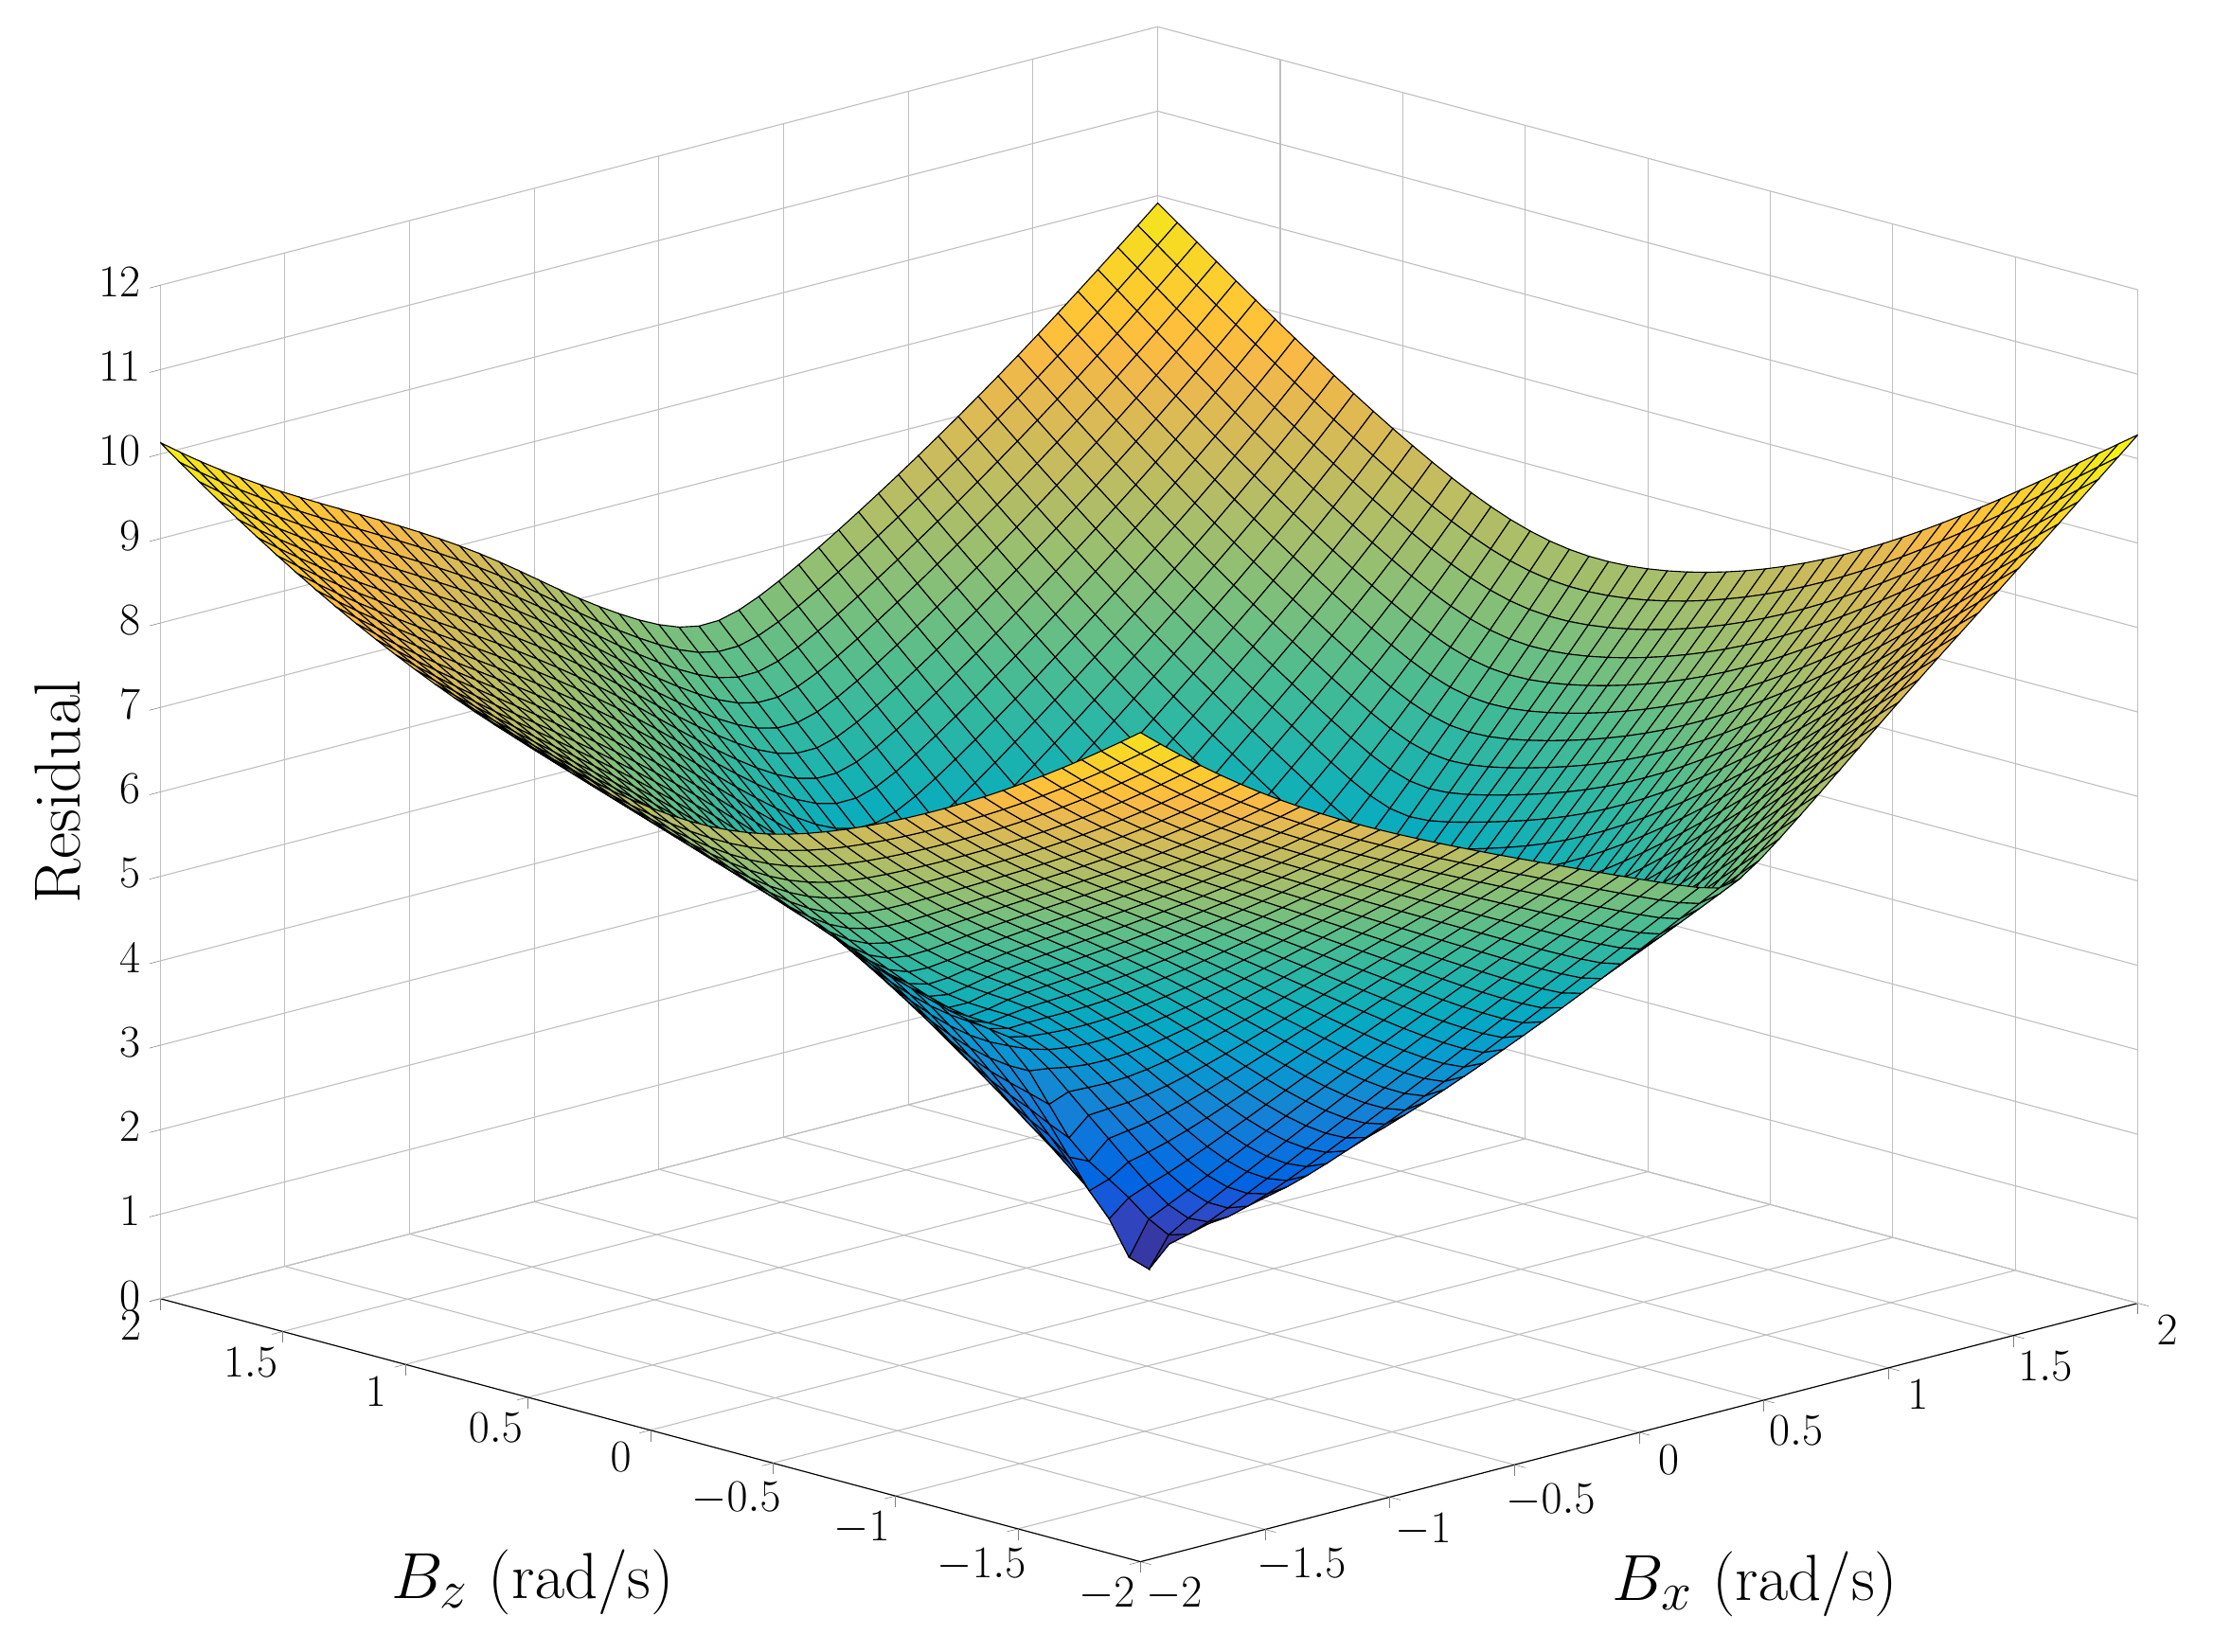
\begin{tikzpicture}

\begin{axis}[%
width=10.442105in,
height=8.107105in,
at={(1.751579in,1.09421in)},
scale only axis,
xmin=-2,
xmax=2,
tick align=outside,
xlabel={\Huge $B_x$ (rad/s)},
xmajorgrids,
ymin=-2,
ymax=2,
ticklabel style = {font=\LARGE},
ylabel={\Huge $B_z$ (rad/s)},
zlabel={\Huge Residual},
ymajorgrids,
zmin=0,
zmax=12,
zmajorgrids,
view={-44.5}{20},
axis x line*=bottom,
axis y line*=left,
axis z line*=left
]

\addplot3[%
surf,
faceted color=black,
shader=faceted,
colormap={mymap}{[1pt] rgb(0pt)=(0.2081,0.1663,0.5292); rgb(1pt)=(0.211624,0.189781,0.577676); rgb(2pt)=(0.212252,0.213771,0.626971); rgb(3pt)=(0.2081,0.2386,0.677086); rgb(4pt)=(0.195905,0.264457,0.7279); rgb(5pt)=(0.170729,0.291938,0.779248); rgb(6pt)=(0.125271,0.324243,0.830271); rgb(7pt)=(0.0591333,0.359833,0.868333); rgb(8pt)=(0.0116952,0.38751,0.881957); rgb(9pt)=(0.00595714,0.408614,0.882843); rgb(10pt)=(0.0165143,0.4266,0.878633); rgb(11pt)=(0.0328524,0.443043,0.871957); rgb(12pt)=(0.0498143,0.458571,0.864057); rgb(13pt)=(0.0629333,0.47369,0.855438); rgb(14pt)=(0.0722667,0.488667,0.8467); rgb(15pt)=(0.0779429,0.503986,0.838371); rgb(16pt)=(0.0793476,0.520024,0.831181); rgb(17pt)=(0.0749429,0.537543,0.826271); rgb(18pt)=(0.0640571,0.556986,0.823957); rgb(19pt)=(0.0487714,0.577224,0.822829); rgb(20pt)=(0.0343429,0.596581,0.819852); rgb(21pt)=(0.0265,0.6137,0.8135); rgb(22pt)=(0.0238905,0.628662,0.803762); rgb(23pt)=(0.0230905,0.641786,0.791267); rgb(24pt)=(0.0227714,0.653486,0.776757); rgb(25pt)=(0.0266619,0.664195,0.760719); rgb(26pt)=(0.0383714,0.674271,0.743552); rgb(27pt)=(0.0589714,0.683757,0.725386); rgb(28pt)=(0.0843,0.692833,0.706167); rgb(29pt)=(0.113295,0.7015,0.685857); rgb(30pt)=(0.145271,0.709757,0.664629); rgb(31pt)=(0.180133,0.717657,0.642433); rgb(32pt)=(0.217829,0.725043,0.619262); rgb(33pt)=(0.258643,0.731714,0.595429); rgb(34pt)=(0.302171,0.737605,0.571186); rgb(35pt)=(0.348167,0.742433,0.547267); rgb(36pt)=(0.395257,0.7459,0.524443); rgb(37pt)=(0.44201,0.748081,0.503314); rgb(38pt)=(0.487124,0.749062,0.483976); rgb(39pt)=(0.530029,0.749114,0.466114); rgb(40pt)=(0.570857,0.748519,0.44939); rgb(41pt)=(0.609852,0.747314,0.433686); rgb(42pt)=(0.6473,0.7456,0.4188); rgb(43pt)=(0.683419,0.743476,0.404433); rgb(44pt)=(0.71841,0.741133,0.390476); rgb(45pt)=(0.752486,0.7384,0.376814); rgb(46pt)=(0.785843,0.735567,0.363271); rgb(47pt)=(0.818505,0.732733,0.34979); rgb(48pt)=(0.850657,0.7299,0.336029); rgb(49pt)=(0.882433,0.727433,0.3217); rgb(50pt)=(0.913933,0.725786,0.306276); rgb(51pt)=(0.944957,0.726114,0.288643); rgb(52pt)=(0.973895,0.731395,0.266648); rgb(53pt)=(0.993771,0.745457,0.240348); rgb(54pt)=(0.999043,0.765314,0.216414); rgb(55pt)=(0.995533,0.786057,0.196652); rgb(56pt)=(0.988,0.8066,0.179367); rgb(57pt)=(0.978857,0.827143,0.163314); rgb(58pt)=(0.9697,0.848138,0.147452); rgb(59pt)=(0.962586,0.870514,0.1309); rgb(60pt)=(0.958871,0.8949,0.113243); rgb(61pt)=(0.959824,0.921833,0.0948381); rgb(62pt)=(0.9661,0.951443,0.0755333); rgb(63pt)=(0.9763,0.9831,0.0538)},
mesh/rows=51]
table[row sep=crcr,header=false] {%
%
-2	-2	9.81858362594526\\
-2	-1.92	9.64452251728806\\
-2	-1.84	9.47451042562919\\
-2	-1.76	9.30897357407741\\
-2	-1.68	9.14825113661622\\
-2	-1.6	8.99260351376251\\
-2	-1.52	8.84222116992727\\
-2	-1.44	8.69723328033107\\
-2	-1.36	8.5577167289465\\
-2	-1.28	8.42370732553334\\
-2	-1.2	8.29521638716627\\
-2	-1.12	8.17225684151268\\
-2	-1.04	8.05488329952717\\
-2	-0.96	7.94324934121235\\
-2	-0.88	7.83768148771943\\
-2	-0.8	7.73876189649163\\
-2	-0.72	7.6474004132146\\
-2	-0.64	7.56486345869347\\
-2	-0.56	7.49271930441668\\
-2	-0.48	7.43266869907617\\
-2	-0.4	7.38626728017591\\
-2	-0.32	7.35460581285723\\
-2	-0.24	7.33806190948509\\
-2	-0.16	7.33622743247058\\
-2	-0.0800000000000001	7.34803960803832\\
-2	0	7.37204992739975\\
-2	0.0800000000000001	7.40671841229014\\
-2	0.16	7.45064145302155\\
-2	0.24	7.50267658343428\\
-2	0.32	7.56197510839651\\
-2	0.4	7.6279549135891\\
-2	0.48	7.70024555976025\\
-2	0.56	7.77862794807303\\
-2	0.64	7.86298042142257\\
-2	0.72	7.95323583141103\\
-2	0.8	8.04935008817921\\
-2	0.88	8.15128096909185\\
-2	0.96	8.25897540731465\\
-2	1.04	8.37236341707586\\
-2	1.12	8.49135691596668\\
-2	1.2	8.61585187126428\\
-2	1.28	8.74573240363427\\
-2	1.36	8.8808757132924\\
-2	1.44	9.02115692606443\\
-2	1.52	9.16645316113722\\
-2	1.6	9.31664627681129\\
-2	1.68	9.47162384631181\\
-2	1.76	9.63127795781556\\
-2	1.84	9.79550143972848\\
-2	1.92	9.96418111559729\\
-2	2	10.1371877394937\\
-1.92	-2	9.62072827943282\\
-1.92	-1.92	9.44476224015503\\
-1.92	-1.84	9.27318306420032\\
-1.92	-1.76	9.10632192357821\\
-1.92	-1.68	8.94442811476345\\
-1.92	-1.6	8.7876778037826\\
-1.92	-1.52	8.63618094547352\\
-1.92	-1.44	8.48998635675636\\
-1.92	-1.36	8.34908630684217\\
-1.92	-1.28	8.21342348973193\\
-1.92	-1.2	8.08290484410577\\
-1.92	-1.12	7.95742818832337\\
-1.92	-1.04	7.83692855706609\\
-1.92	-0.96	7.72145054386162\\
-1.92	-0.88	7.61124937197518\\
-1.92	-0.8	7.50691471890585\\
-1.92	-0.72	7.40949535710895\\
-1.92	-0.64	7.32057959852148\\
-1.92	-0.56	7.24226397537107\\
-1.92	-0.48	7.17694142044283\\
-1.92	-0.4	7.12688995105143\\
-1.92	-0.32	7.09375155635508\\
-1.92	-0.24	7.07810222741461\\
-1.92	-0.16	7.07932039342285\\
-1.92	-0.0800000000000001	7.09581636221096\\
-1.92	0	7.12549220622676\\
-1.92	0.0800000000000001	7.16621488758928\\
-1.92	0.16	7.21614441496019\\
-1.92	0.24	7.27387637294788\\
-1.92	0.32	7.33844175964963\\
-1.92	0.4	7.40923120341209\\
-1.92	0.48	7.48589711848852\\
-1.92	0.56	7.56826379034856\\
-1.92	0.64	7.65625665800415\\
-1.92	0.72	7.74985157610403\\
-1.92	0.8	7.84904070420502\\
-1.92	0.88	7.95381101030239\\
-1.92	0.96	8.06413204533799\\
-1.92	1.04	8.17995049646661\\
-1.92	1.12	8.30118964691377\\
-1.92	1.2	8.42775223922347\\
-1.92	1.28	8.55952546711661\\
-1.92	1.36	8.69638700784915\\
-1.92	1.44	8.83821119430403\\
-1.92	1.52	8.98487461028399\\
-1.92	1.6	9.13626055006186\\
-1.92	1.68	9.29226189216986\\
-1.92	1.76	9.45278198758106\\
-1.92	1.84	9.6177331583979\\
-1.92	1.92	9.78703236419152\\
-1.92	2	9.96059355444391\\
-1.84	-2	9.42958185758455\\
-1.84	-1.92	9.25241430493342\\
-1.84	-1.84	9.07987872505827\\
-1.84	-1.76	8.9122191040566\\
-1.84	-1.68	8.74960605215552\\
-1.84	-1.6	8.59214350500812\\
-1.84	-1.52	8.43987165721111\\
-1.84	-1.44	8.29276676645096\\
-1.84	-1.36	8.1507398773119\\
-1.84	-1.28	8.01363815714022\\
-1.84	-1.2	7.88125443019348\\
-1.84	-1.12	7.75335249334267\\
-1.84	-1.04	7.6297174990978\\
-1.84	-0.96	7.51024129625691\\
-1.84	-0.88	7.39505055203036\\
-1.84	-0.8	7.2846777305677\\
-1.84	-0.72	7.18025659999581\\
-1.84	-0.64	7.08368961849506\\
-1.84	-0.56	6.99768688587308\\
-1.84	-0.48	6.92554288824132\\
-1.84	-0.4	6.87056179429043\\
-1.84	-0.32	6.83522260917249\\
-1.84	-0.24	6.82042498432924\\
-1.84	-0.16	6.82523358429723\\
-1.84	-0.0800000000000001	6.84727261878999\\
-1.84	0	6.8835149728452\\
-1.84	0.0800000000000001	6.93104162780636\\
-1.84	0.16	6.98750033884757\\
-1.84	0.24	7.05123878144306\\
-1.84	0.32	7.12122690989717\\
-1.84	0.4	7.19689625684853\\
-1.84	0.48	7.2779786888551\\
-1.84	0.56	7.36437966524874\\
-1.84	0.64	7.45609141474777\\
-1.84	0.72	7.55313867228003\\
-1.84	0.8	7.65554696765978\\
-1.84	0.88	7.76332520269248\\
-1.84	0.96	7.87645703136576\\
-1.84	1.04	7.99489785864886\\
-1.84	1.12	8.11857569267493\\
-1.84	1.2	8.24739475720793\\
-1.84	1.28	8.38124100175165\\
-1.84	1.36	8.51998870648356\\
-1.84	1.44	8.66350742690918\\
-1.84	1.52	8.81166861034928\\
-1.84	1.6	8.96435132969956\\
-1.84	1.68	9.12144668341082\\
-1.84	1.76	9.28286047285236\\
-1.84	1.84	9.44851377332635\\
-1.84	1.92	9.61834096495228\\
-1.84	2	9.79228470415869\\
-1.76	-2	9.24599749199039\\
-1.76	-1.92	9.06817847798293\\
-1.76	-1.84	8.89514893860007\\
-1.76	-1.76	8.72707880272569\\
-1.76	-1.68	8.56407422667687\\
-1.76	-1.6	8.40618043475322\\
-1.76	-1.52	8.25337939271105\\
-1.76	-1.44	8.10558349897486\\
-1.76	-1.36	7.96262787366028\\
-1.76	-1.28	7.82426552527189\\
-1.76	-1.2	7.69017169544775\\
-1.76	-1.12	7.55996593875198\\
-1.76	-1.04	7.43326283017622\\
-1.76	-0.96	7.30976431752571\\
-1.76	-0.88	7.18940773088074\\
-1.76	-0.8	7.07258031304229\\
-1.76	-0.72	6.96039611690162\\
-1.76	-0.64	6.85499005763049\\
-1.76	-0.56	6.75970339780816\\
-1.76	-0.48	6.67893385817182\\
-1.76	-0.4	6.61740804788113\\
-1.76	-0.32	6.57888513994448\\
-1.76	-0.24	6.56482322784101\\
-1.76	-0.16	6.57385004314659\\
-1.76	-0.0800000000000001	6.60242342824194\\
-1.76	0	6.6461904563035\\
-1.76	0.0800000000000001	6.70120537035245\\
-1.76	0.16	6.76454530299362\\
-1.76	0.24	6.83437157299014\\
-1.76	0.32	6.90969981120744\\
-1.76	0.4	6.99010442023435\\
-1.76	0.48	7.07547187351645\\
-1.76	0.56	7.16583330941293\\
-1.76	0.64	7.26126642307905\\
-1.76	0.72	7.36184520825638\\
-1.76	0.8	7.46761797004038\\
-1.76	0.88	7.57859991305769\\
-1.76	0.96	7.69477233446895\\
-1.76	1.04	7.8160846082841\\
-1.76	1.12	7.94245758320364\\
-1.76	1.2	8.07378809497033\\
-1.76	1.28	8.20995453365817\\
-1.76	1.36	8.35082327249247\\
-1.76	1.44	8.49625557009369\\
-1.76	1.52	8.64611444697345\\
-1.76	1.6	8.80027103010947\\
-1.76	1.68	8.95860991415436\\
-1.76	1.76	9.12103314822669\\
-1.76	1.84	9.28746248012253\\
-1.76	1.92	9.45783945357119\\
-1.76	2	9.63212285894053\\
-1.68	-2	9.07046997059456\\
-1.68	-1.92	8.89239058695296\\
-1.68	-1.84	8.71917980384441\\
-1.68	-1.76	8.55094859735909\\
-1.68	-1.68	8.38775318428694\\
-1.68	-1.6	8.22959298464785\\
-1.68	-1.52	8.07640263543276\\
-1.68	-1.44	7.92803970989147\\
-1.68	-1.36	7.78427113254406\\
-1.68	-1.28	7.64476288243784\\
-1.68	-1.2	7.50907939807145\\
-1.68	-1.12	7.37670110653116\\
-1.68	-1.04	7.24707090960335\\
-1.68	-0.96	7.11968390262435\\
-1.68	-0.88	6.99423973215702\\
-1.68	-0.8	6.87088250134231\\
-1.68	-0.72	6.75055074543624\\
-1.68	-0.64	6.63542640500719\\
-1.68	-0.56	6.52936528625949\\
-1.68	-0.48	6.43798623516067\\
-1.68	-0.4	6.367907351343\\
-1.68	-0.32	6.32484313012476\\
-1.68	-0.24	6.31125558050018\\
-1.68	-0.16	6.32521320337795\\
-1.68	-0.0800000000000001	6.36145338325193\\
-1.68	0	6.4137350301967\\
-1.68	0.0800000000000001	6.47679341882981\\
-1.68	0.16	6.54711815602944\\
-1.68	0.24	6.62281634637857\\
-1.68	0.32	6.70311373265424\\
-1.68	0.4	6.78786273356612\\
-1.68	0.48	6.87719266252206\\
-1.68	0.56	6.97130585024017\\
-1.68	0.64	7.07037925645264\\
-1.68	0.72	7.17452922149423\\
-1.68	0.8	7.28380813608096\\
-1.68	0.88	7.3982137099551\\
-1.68	0.96	7.51770065207318\\
-1.68	1.04	7.64219060203736\\
-1.68	1.12	7.77157959253582\\
-1.68	1.2	7.90574384829541\\
-1.68	1.28	8.04454501630206\\
-1.68	1.36	8.18783558484568\\
-1.68	1.44	8.33546474563607\\
-1.68	1.52	8.48728454851085\\
-1.68	1.6	8.64315597936114\\
-1.68	1.68	8.80295453109644\\
-1.68	1.76	8.96657486012519\\
-1.68	1.84	9.13393415299265\\
-1.68	1.92	9.30497381811398\\
-1.68	2	9.47965904152775\\
-1.6	-2	8.90316326599343\\
-1.6	-1.92	8.72505952396865\\
-1.6	-1.84	8.55183510914483\\
-1.6	-1.76	8.38355645928275\\
-1.6	-1.68	8.22024255267887\\
-1.6	-1.6	8.0618577642473\\
-1.6	-1.52	7.90829868997939\\
-1.6	-1.44	7.7593770585549\\
-1.6	-1.36	7.61480206460552\\
-1.6	-1.28	7.47416674476976\\
-1.6	-1.2	7.33694419696917\\
-1.6	-1.12	7.20250051472913\\
-1.6	-1.04	7.07013291207882\\
-1.6	-0.96	6.93914542308751\\
-1.6	-0.88	6.8089836498678\\
-1.6	-0.8	6.67946654143432\\
-1.6	-0.72	6.55117274759631\\
-1.6	-0.64	6.42603608806453\\
-1.6	-0.56	6.30810756323179\\
-1.6	-0.48	6.2041318157686\\
-1.6	-0.4	6.12306658231255\\
-1.6	-0.32	6.07355811222919\\
-1.6	-0.24	6.05990355072825\\
-1.6	-0.16	6.07955899940081\\
-1.6	-0.0800000000000001	6.12473814510351\\
-1.6	0	6.18651123491969\\
-1.6	0.0800000000000001	6.25795362721679\\
-1.6	0.16	6.33503085905298\\
-1.6	0.24	6.41602691191356\\
-1.6	0.32	6.50060564691237\\
-1.6	0.4	6.58905747598954\\
-1.6	0.48	6.6818437292363\\
-1.6	0.56	6.7793745476283\\
-1.6	0.64	6.88192931664676\\
-1.6	0.72	6.98965055254458\\
-1.6	0.8	7.10256854463321\\
-1.6	0.88	7.22063338134154\\
-1.6	0.96	7.3437432068127\\
-1.6	1.04	7.47176483757517\\
-1.6	1.12	7.60454691986859\\
-1.6	1.2	7.74192766740735\\
-1.6	1.28	7.88373960447699\\
-1.6	1.36	8.02981326777595\\
-1.6	1.44	8.17998102474523\\
-1.6	1.52	8.33408142285217\\
-1.6	1.6	8.49196397627905\\
-1.6	1.68	8.65349404358423\\
-1.6	1.76	8.81855737914775\\
-1.6	1.84	8.98706395374486\\
-1.6	1.92	9.15895065181282\\
-1.6	2	9.33418241140666\\
-1.52	-2	8.74395720988307\\
-1.52	-1.92	8.56592062123873\\
-1.52	-1.84	8.39271433397623\\
-1.52	-1.76	8.22437213189908\\
-1.52	-1.68	8.06088533536897\\
-1.52	-1.6	7.90219102976647\\
-1.52	-1.52	7.74815495349049\\
-1.52	-1.44	7.59855168757624\\
-1.52	-1.36	7.45304579653618\\
-1.52	-1.28	7.31117828558101\\
-1.52	-1.2	7.17236281923253\\
-1.52	-1.12	7.03589561218789\\
-1.52	-1.04	6.90098279777838\\
-1.52	-0.96	6.76679219493669\\
-1.52	-0.88	6.63254770869951\\
-1.52	-0.8	6.49771068500152\\
-1.52	-0.72	6.36233754037628\\
-1.52	-0.64	6.22775291522867\\
-1.52	-0.56	6.09765384799996\\
-1.52	-0.48	5.97943651138113\\
-1.52	-0.4	5.88459734304274\\
-1.52	-0.32	5.82598080990251\\
-1.52	-0.24	5.81121003096917\\
-1.52	-0.16	5.83731268390938\\
-1.52	-0.0800000000000001	5.89282367988377\\
-1.52	0	5.96497656352559\\
-1.52	0.0800000000000001	6.04481321234181\\
-1.52	0.16	6.12797929466364\\
-1.52	0.24	6.21329700560712\\
-1.52	0.32	6.30115615073023\\
-1.52	0.4	6.39245073642263\\
-1.52	0.48	6.48804483459241\\
-1.52	0.56	6.58857057723388\\
-1.52	0.64	6.69439519996205\\
-1.52	0.72	6.80565991753708\\
-1.52	0.8	6.92234050316326\\
-1.52	0.88	7.0443060068163\\
-1.52	0.96	7.17136586182239\\
-1.52	1.04	7.30330283844437\\
-1.52	1.12	7.43989315403637\\
-1.52	1.2	7.58091691870771\\
-1.52	1.28	7.72616257463952\\
-1.52	1.36	7.87542851000797\\
-1.52	1.44	8.02852405763144\\
-1.52	1.52	8.18527105093235\\
-1.52	1.6	8.34550628805575\\
-1.52	1.68	8.5090847499502\\
-1.52	1.76	8.67588319128959\\
-1.52	1.84	8.84580366968017\\
-1.52	1.92	9.0187765888977\\
-1.52	2	9.19476282247127\\
-1.44	-2	8.59250529549857\\
-1.44	-1.92	8.41449814278725\\
-1.44	-1.84	8.24121898971336\\
-1.44	-1.76	8.07267736403387\\
-1.44	-1.68	7.90884290029524\\
-1.44	-1.6	7.74962999597907\\
-1.44	-1.52	7.59487862457522\\
-1.44	-1.44	7.44433454853305\\
-1.44	-1.36	7.29763285335108\\
-1.44	-1.28	7.15428861631614\\
-1.44	-1.2	7.01369715289053\\
-1.44	-1.12	6.87514374527148\\
-1.44	-1.04	6.73782042638981\\
-1.44	-0.96	6.60084862919805\\
-1.44	-0.88	6.46331733343423\\
-1.44	-0.8	6.3243763872815\\
-1.44	-0.72	6.18348793924656\\
-1.44	-0.64	6.04104672785002\\
-1.44	-0.56	5.89969333623318\\
-1.44	-0.48	5.76650258709616\\
-1.44	-0.4	5.65506417048346\\
-1.44	-0.32	5.58371936096778\\
-1.44	-0.24	5.56591699913917\\
-1.44	-0.16	5.59905628393265\\
-1.44	-0.0800000000000001	5.66636444712718\\
-1.44	0	5.74957521112203\\
-1.44	0.0800000000000001	5.83733273933093\\
-1.44	0.16	5.9253962919581\\
-1.44	0.24	6.01364406732325\\
-1.44	0.32	6.10351740458478\\
-1.44	0.4	6.19665206449282\\
-1.44	0.48	6.29434159638638\\
-1.44	0.56	6.39741698631935\\
-1.44	0.64	6.50629435314762\\
-1.44	0.72	6.62107347181055\\
-1.44	0.8	6.74163879427286\\
-1.44	0.88	6.86774524701518\\
-1.44	0.96	6.9990836224114\\
-1.44	1.04	7.13532563579773\\
-1.44	1.12	7.27615129295435\\
-1.44	1.2	7.42126260021761\\
-1.44	1.28	7.57038813398361\\
-1.44	1.36	7.72328263677625\\
-1.44	1.44	7.87972485219752\\
-1.44	1.52	8.03951562099563\\
-1.44	1.6	8.20247718137831\\
-1.44	1.68	8.36845384632523\\
-1.44	1.76	8.53731379971905\\
-1.44	1.84	8.70895158157959\\
-1.44	1.92	8.88329080189264\\
-1.44	2	9.06028662517392\\
-1.36	-2	8.44829620021191\\
-1.36	-1.92	8.27016995391386\\
-1.36	-1.84	8.09662056315456\\
-1.36	-1.76	7.92763807925874\\
-1.36	-1.68	7.76317307194307\\
-1.36	-1.6	7.60311917653715\\
-1.36	-1.52	7.44729405358081\\
-1.36	-1.44	7.29542263691801\\
-1.36	-1.36	7.14712674349885\\
-1.36	-1.28	7.00192398018009\\
-1.36	-1.2	6.85923591951437\\
-1.36	-1.12	6.71840102471286\\
-1.36	-1.04	6.57868342773275\\
-1.36	-0.96	6.43926772201286\\
-1.36	-0.88	6.29923785747888\\
-1.36	-0.8	6.1575646231604\\
-1.36	-0.72	6.01319083668812\\
-1.36	-0.64	5.86544499747224\\
-1.36	-0.56	5.71527559744725\\
-1.36	-0.48	5.56805096989368\\
-1.36	-0.4	5.4379113140202\\
-1.36	-0.32	5.34927313402107\\
-1.36	-0.24	5.3251422970564\\
-1.36	-0.16	5.36548475466873\\
-1.36	-0.0800000000000001	5.4460300708287\\
-1.36	0	5.54057576860781\\
-1.36	0.0800000000000001	5.63510271520774\\
-1.36	0.16	5.72626536526904\\
-1.36	0.24	5.81567468792525\\
-1.36	0.32	5.90613463959295\\
-1.36	0.4	6.00008576167053\\
-1.36	0.48	6.0992062191695\\
-1.36	0.56	6.20445339048251\\
-1.36	0.64	6.31622547724005\\
-1.36	0.72	6.43452861989389\\
-1.36	0.8	6.55911728973639\\
-1.36	0.88	6.689603157401\\
-1.36	0.96	6.82553493209599\\
-1.36	1.04	6.96645298980714\\
-1.36	1.12	7.11192289114698\\
-1.36	1.2	7.26155228767799\\
-1.36	1.28	7.41499604044472\\
-1.36	1.36	7.57195422894911\\
-1.36	1.44	7.73216698813189\\
-1.36	1.52	7.89540897168567\\
-1.36	1.6	8.06148503994429\\
-1.36	1.68	8.23022778786252\\
-1.36	1.76	8.401496884353\\
-1.36	1.84	8.57517986535109\\
-1.36	1.92	8.75119390802606\\
-1.36	2	8.92948809610896\\
-1.28	-2	8.31071276152542\\
-1.28	-1.92	8.13222834580699\\
-1.28	-1.84	7.95812392363688\\
-1.28	-1.76	7.78837176586093\\
-1.28	-1.68	7.62290347579278\\
-1.28	-1.6	7.46159210556637\\
-1.28	-1.52	7.30423554934693\\
-1.28	-1.44	7.15054565055155\\
-1.28	-1.36	7.00014700619275\\
-1.28	-1.28	6.85258716009672\\
-1.28	-1.2	6.7073554376956\\
-1.28	-1.12	6.56390176604239\\
-1.28	-1.04	6.42164131089591\\
-1.28	-0.96	6.27992837431857\\
-1.28	-0.88	6.13798713591227\\
-1.28	-0.8	5.99480373095727\\
-1.28	-0.72	5.84903167719073\\
-1.28	-0.64	5.6990924900931\\
-1.28	-0.56	5.54398768500713\\
-1.28	-0.48	5.38602679739993\\
-1.28	-0.4	5.23713968345641\\
-1.28	-0.32	5.12631703723\\
-1.28	-0.24	5.09055949770474\\
-1.28	-0.16	5.13737820231134\\
-1.28	-0.0800000000000001	5.23239130640063\\
-1.28	0	5.33785771599602\\
-1.28	0.0800000000000001	5.43709879943917\\
-1.28	0.16	5.52892901331764\\
-1.28	0.24	5.61747195870976\\
-1.28	0.32	5.70709725928575\\
-1.28	0.4	5.80098135220847\\
-1.28	0.48	5.90104906494395\\
-1.28	0.56	6.00825885537339\\
-1.28	0.64	6.12289903188979\\
-1.28	0.72	6.24482155154852\\
-1.28	0.8	6.3736137438716\\
-1.28	0.88	6.50872195419666\\
-1.28	0.96	6.64953912766896\\
-1.28	1.04	6.79546437103711\\
-1.28	1.12	6.94593997747355\\
-1.28	1.2	7.10047049819822\\
-1.28	1.28	7.25862843668004\\
-1.28	1.36	7.42005118581541\\
-1.28	1.44	7.58443342868613\\
-1.28	1.52	7.75151832784431\\
-1.28	1.6	7.92108968339627\\
-1.28	1.68	8.09296615705436\\
-1.28	1.76	8.26699784389567\\
-1.28	1.84	8.44306498038623\\
-1.28	1.92	8.62107834875684\\
-1.28	2	8.80098086869809\\
-1.2	-2	8.17908376787939\\
-1.2	-1.92	7.99993251748862\\
-1.2	-1.84	7.82492147241427\\
-1.2	-1.76	7.65400471162734\\
-1.2	-1.68	7.48709360897287\\
-1.2	-1.6	7.32404020895373\\
-1.2	-1.52	7.16462510577933\\
-1.2	-1.44	7.00855461384444\\
-1.2	-1.36	6.85547075349801\\
-1.2	-1.28	6.70497412650357\\
-1.2	-1.2	6.5566542113525\\
-1.2	-1.12	6.41011517861897\\
-1.2	-1.04	6.2649800260698\\
-1.2	-0.96	6.12085344125297\\
-1.2	-0.88	5.97722504179377\\
-1.2	-0.8	5.83330072669038\\
-1.2	-0.72	5.6877703341803\\
-1.2	-0.64	5.53859710641221\\
-1.2	-0.56	5.38319407242925\\
-1.2	-0.48	5.22022894577237\\
-1.2	-0.4	5.05623702214341\\
-1.2	-0.32	4.91984670580093\\
-1.2	-0.24	4.86476479440286\\
-1.2	-0.16	4.91562498482811\\
-1.2	-0.0800000000000001	5.02578751501985\\
-1.2	0	5.14064259507277\\
-1.2	0.0800000000000001	5.24142119077197\\
-1.2	0.16	5.33094011449892\\
-1.2	0.24	5.41655283739831\\
-1.2	0.32	5.50415577700634\\
-1.2	0.4	5.5974112892754\\
-1.2	0.48	5.69825624266469\\
-1.2	0.56	5.80748218713479\\
-1.2	0.64	5.9251607785262\\
-1.2	0.72	6.05092795090072\\
-1.2	0.8	6.18417222098714\\
-1.2	0.88	6.32416179637587\\
-1.2	0.96	6.47013156749698\\
-1.2	1.04	6.62134167552562\\
-1.2	1.12	6.77711417724988\\
-1.2	1.2	6.93685218094655\\
-1.2	1.28	7.10004540065892\\
-1.2	1.36	7.2662662236702\\
-1.2	1.44	7.43516033159901\\
-1.2	1.52	7.60643536484214\\
-1.2	1.6	7.77985017599643\\
-1.2	1.68	7.95520616490638\\
-1.2	1.76	8.13234128569056\\
-1.2	1.84	8.31112669512705\\
-1.2	1.92	8.49146567315855\\
-1.2	2	8.67329431289817\\
-1.12	-2	8.05272580400518\\
-1.12	-1.92	7.87255007901515\\
-1.12	-1.84	7.69623521785385\\
-1.12	-1.76	7.52371575901154\\
-1.12	-1.68	7.35488146137149\\
-1.12	-1.6	7.18956344603846\\
-1.12	-1.52	7.02752810760806\\
-1.12	-1.44	6.86848359290392\\
-1.12	-1.36	6.71210146764031\\
-1.12	-1.28	6.55805172819385\\
-1.12	-1.2	6.40604323363765\\
-1.12	-1.12	6.25585570133528\\
-1.12	-1.04	6.1073456242044\\
-1.12	-0.96	5.96040751364699\\
-1.12	-0.88	5.81487207148659\\
-1.12	-0.8	5.6703211005132\\
-1.12	-0.72	5.52579529676516\\
-1.12	-0.64	5.37938507389921\\
-1.12	-0.56	5.2278277973815\\
-1.12	-0.48	5.06690688007164\\
-1.12	-0.4	4.89600733205659\\
-1.12	-0.32	4.7355608195278\\
-1.12	-0.24	4.65188145729007\\
-1.12	-0.16	4.70133828033959\\
-1.12	-0.0800000000000001	4.8261568972494\\
-1.12	0	4.94715809838447\\
-1.12	0.0800000000000001	5.04506247805508\\
-1.12	0.16	5.12901906366446\\
-1.12	0.24	5.20994137656158\\
-1.12	0.32	5.29482914622918\\
-1.12	0.4	5.38738703866901\\
-1.12	0.48	5.48925834478923\\
-1.12	0.56	5.60088267441375\\
-1.12	0.64	5.72201054263027\\
-1.12	0.72	5.85200802784109\\
-1.12	0.8	5.99004271250121\\
-1.12	0.88	6.1352021880261\\
-1.12	0.96	6.28657219499809\\
-1.12	1.04	6.44328816595953\\
-1.12	1.12	6.60456712036904\\
-1.12	1.2	6.76972390455512\\
-1.12	1.28	6.93817499414016\\
-1.12	1.36	7.10943322700751\\
-1.12	1.44	7.28309701512926\\
-1.12	1.52	7.45883733852238\\
-1.12	1.6	7.6363851216007\\
-1.12	1.68	7.81552065601172\\
-1.12	1.76	7.99606583843824\\
-1.12	1.84	8.17787931842037\\
-1.12	1.92	8.36085425118958\\
-1.12	2	8.54491817707997\\
-1.04	-2	7.93097419866809\\
-1.04	-1.92	7.7493867721146\\
-1.04	-1.84	7.57134591193632\\
-1.04	-1.76	7.39676546276879\\
-1.04	-1.68	7.22551314768954\\
-1.04	-1.6	7.05740062244499\\
-1.04	-1.52	6.89218424629163\\
-1.04	-1.44	6.72958095714422\\
-1.04	-1.36	6.56930055434194\\
-1.04	-1.28	6.4110905211216\\
-1.04	-1.2	6.25478356277226\\
-1.04	-1.12	6.10033347626094\\
-1.04	-1.04	5.94782351831964\\
-1.04	-0.96	5.79743271057462\\
-1.04	-0.88	5.64934629020139\\
-1.04	-0.8	5.50359146660303\\
-1.04	-0.72	5.35976316609698\\
-1.04	-0.64	5.21657561703287\\
-1.04	-0.56	5.07116733148111\\
-1.04	-0.48	4.91833803467461\\
-1.04	-0.4	4.75172161492667\\
-1.04	-0.32	4.57723224749107\\
-1.04	-0.24	4.45815213611436\\
-1.04	-0.16	4.49611339955172\\
-1.04	-0.0800000000000001	4.63277359562731\\
-1.04	0	4.7542305017225\\
-1.04	0.0800000000000001	4.84378391914391\\
-1.04	0.16	4.91918626380859\\
-1.04	0.24	4.9943855414086\\
-1.04	0.32	5.07660344533803\\
-1.04	0.4	5.16900573303799\\
-1.04	0.48	5.27262330405947\\
-1.04	0.56	5.38737807651877\\
-1.04	0.64	5.51261655837635\\
-1.04	0.72	5.64739826112979\\
-1.04	0.8	5.79066057597658\\
-1.04	0.88	5.94131840895809\\
-1.04	0.96	6.09832685862017\\
-1.04	1.04	6.26072069579902\\
-1.04	1.12	6.42763732589564\\
-1.04	1.2	6.59832680060864\\
-1.04	1.28	6.77215153516717\\
-1.04	1.36	6.94857848888838\\
-1.04	1.44	7.12716680977458\\
-1.04	1.52	7.30755383346448\\
-1.04	1.6	7.4894417690164\\
-1.04	1.68	7.6725865819498\\
-1.04	1.76	7.85678976294089\\
-1.04	1.84	8.04189304093507\\
-1.04	1.92	8.22777572820345\\
-1.04	2	8.41435423544237\\
-0.96	-2	7.81320360174952\\
-0.96	-1.92	7.62980512046576\\
-0.96	-1.84	7.44961004001452\\
-0.96	-1.76	7.27251145658951\\
-0.96	-1.68	7.09835635426243\\
-0.96	-1.6	6.92694021499394\\
-0.96	-1.52	6.75801462852532\\
-0.96	-1.44	6.59131146950809\\
-0.96	-1.36	6.42658337425034\\
-0.96	-1.28	6.2636548123332\\
-0.96	-1.2	6.10247284587232\\
-0.96	-1.12	5.94314399532461\\
-0.96	-1.04	5.78594464544231\\
-0.96	-0.96	5.63129582143101\\
-0.96	-0.88	5.47969514534517\\
-0.96	-0.8	5.33159405605939\\
-0.96	-0.72	5.1871904434284\\
-0.96	-0.64	5.04606610318935\\
-0.96	-0.56	4.90652280447927\\
-0.96	-0.48	4.7643998926807\\
-0.96	-0.4	4.61169294675243\\
-0.96	-0.32	4.44115859240603\\
-0.96	-0.24	4.29107741548145\\
-0.96	-0.16	4.30242293330682\\
-0.96	-0.0800000000000001	4.44377238932089\\
-0.96	0	4.55684944793094\\
-0.96	0.0800000000000001	4.63222662884575\\
-0.96	0.16	4.69712214538803\\
-0.96	0.24	4.76670697038268\\
-0.96	0.32	4.84719199648772\\
-0.96	0.4	4.9406210642078\\
-0.96	0.48	5.04715721296829\\
-0.96	0.56	5.16609361109958\\
-0.96	0.64	5.29632672093303\\
-0.96	0.72	5.43659603584385\\
-0.96	0.8	5.58561423894354\\
-0.96	0.88	5.74214137895713\\
-0.96	0.96	5.90502791469664\\
-0.96	1.04	6.0732386203201\\
-0.96	1.12	6.24586325722257\\
-0.96	1.2	6.42211724908401\\
-0.96	1.28	6.60133479781102\\
-0.96	1.36	6.78295691713915\\
-0.96	1.44	6.96651697681474\\
-0.96	1.52	7.15162613230783\\
-0.96	1.6	7.33796042239488\\
-0.96	1.68	7.52525054768058\\
-0.96	1.76	7.71327463928215\\
-0.96	1.84	7.90185383956083\\
-0.96	1.92	8.09085027395503\\
-0.96	2	8.28016693714491\\
-0.88	-2	7.69883973713815\\
-0.88	-1.92	7.51323377857968\\
-0.88	-1.84	7.33046664242507\\
-0.88	-1.76	7.15041225458558\\
-0.88	-1.68	6.97290017122623\\
-0.88	-1.6	6.7977147985092\\
-0.88	-1.52	6.6246089586243\\
-0.88	-1.44	6.45333425110704\\
-0.88	-1.36	6.28368638123663\\
-0.88	-1.28	6.11555842904747\\
-0.88	-1.2	5.94899104099867\\
-0.88	-1.12	5.78420780009009\\
-0.88	-1.04	5.62162701099205\\
-0.88	-0.96	5.46184588914949\\
-0.88	-0.88	5.30559604821209\\
-0.88	-0.8	5.15366622973149\\
-0.88	-0.72	5.00677495283005\\
-0.88	-0.64	4.86534379563384\\
-0.88	-0.56	4.72904993076191\\
-0.88	-0.48	4.59587805018835\\
-0.88	-0.4	4.46017511303458\\
-0.88	-0.32	4.31076435556409\\
-0.88	-0.24	4.15305754129724\\
-0.88	-0.16	4.12373129774813\\
-0.88	-0.0800000000000001	4.25522690303962\\
-0.88	0	4.34786810214148\\
-0.88	0.0800000000000001	4.40440241050633\\
-0.88	0.16	4.45874441734031\\
-0.88	0.24	4.52422027962358\\
-0.88	0.32	4.60480058100214\\
-0.88	0.4	4.70100277873077\\
-0.88	0.48	4.81199577560277\\
-0.88	0.56	4.93640797643509\\
-0.88	0.64	5.07268210637779\\
-0.88	0.72	5.21924886973348\\
-0.88	0.8	5.37461673228858\\
-0.88	0.88	5.53741802980903\\
-0.88	0.96	5.70643029098445\\
-0.88	1.04	5.88058232776612\\
-0.88	1.12	6.05895020293107\\
-0.88	1.2	6.24074625874893\\
-0.88	1.28	6.42530379900096\\
-0.88	1.36	6.6120598947039\\
-0.88	1.44	6.80053855611536\\
-0.88	1.52	6.99033598214824\\
-0.88	1.6	7.18110887375947\\
-0.88	1.68	7.3725661027327\\
-0.88	1.76	7.56446352407536\\
-0.88	1.84	7.75660145140847\\
-0.88	1.92	7.94882423345961\\
-0.88	2	8.14102139736716\\
-0.8	-2	7.58736441479624\\
-0.8	-1.92	7.39916991453708\\
-0.8	-1.84	7.21343662026147\\
-0.8	-1.76	7.03002257835995\\
-0.8	-1.68	6.84874502815183\\
-0.8	-1.6	6.66938369529094\\
-0.8	-1.52	6.49169869629439\\
-0.8	-1.44	6.31546427649226\\
-0.8	-1.36	6.14051529510879\\
-0.8	-1.28	5.96679887362325\\
-0.8	-1.2	5.7944210399372\\
-0.8	-1.12	5.62367907964785\\
-0.8	-1.04	5.45507439835288\\
-0.8	-0.96	5.28930581360571\\
-0.8	-0.88	5.1272463359882\\
-0.8	-0.8	4.96990518668167\\
-0.8	-0.72	4.81836907127291\\
-0.8	-0.64	4.67369870983756\\
-0.8	-0.56	4.53671572033114\\
-0.8	-0.48	4.40751162618129\\
-0.8	-0.4	4.28424030414021\\
-0.8	-0.32	4.16038957921474\\
-0.8	-0.24	4.02678104280362\\
-0.8	-0.16	3.96181605973438\\
-0.8	-0.0800000000000001	4.05933900307135\\
-0.8	0	4.11818210544346\\
-0.8	0.0800000000000001	4.15462592947665\\
-0.8	0.16	4.20088699927192\\
-0.8	0.24	4.26511510582657\\
-0.8	0.32	4.34833554216215\\
-0.8	0.4	4.44945642129311\\
-0.8	0.48	4.56667841281841\\
-0.8	0.56	4.6980003929192\\
-0.8	0.64	4.84144441286655\\
-0.8	0.72	4.99516545574661\\
-0.8	0.8	5.15750247216967\\
-0.8	0.88	5.32699615541362\\
-0.8	0.96	5.50238714308088\\
-0.8	1.04	5.68260255763834\\
-0.8	1.12	5.86673581600658\\
-0.8	1.2	6.05402323976922\\
-0.8	1.28	6.24382030294426\\
-0.8	1.36	6.43557974489335\\
-0.8	1.44	6.62883303268932\\
-0.8	1.52	6.82317588131437\\
-0.8	1.6	7.01825791628575\\
-0.8	1.68	7.21377617960416\\
-0.8	1.76	7.40947199799182\\
-0.8	1.84	7.60513065495859\\
-0.8	1.92	7.8005832524582\\
-0.8	2	7.99571008003351\\
-0.72	-2	7.47831596317262\\
-0.72	-1.92	7.28717704552993\\
-0.72	-1.84	7.09811733732889\\
-0.72	-1.76	6.91098361797792\\
-0.72	-1.68	6.72558701703388\\
-0.72	-1.6	6.54170936439408\\
-0.72	-1.52	6.3591233595135\\
-0.72	-1.44	6.17762665633279\\
-0.72	-1.36	5.99708603980431\\
-0.72	-1.28	5.81748439126826\\
-0.72	-1.2	5.63896189388066\\
-0.72	-1.12	5.46184483616331\\
-0.72	-1.04	5.28665969019551\\
-0.72	-0.96	5.11413479046459\\
-0.72	-0.88	4.94519471709594\\
-0.72	-0.8	4.7809521226384\\
-0.72	-0.72	4.62269789582335\\
-0.72	-0.64	4.47188261519881\\
-0.72	-0.56	4.33006677961585\\
-0.72	-0.48	4.19878185470319\\
-0.72	-0.4	4.07914831326662\\
-0.72	-0.32	3.97084976422023\\
-0.72	-0.24	3.87076211111385\\
-0.72	-0.16	3.80316684689592\\
-0.72	-0.0800000000000001	3.84103844363037\\
-0.72	0	3.85783577837236\\
-0.72	0.0800000000000001	3.878719906854\\
-0.72	0.16	3.92187033485071\\
-0.72	0.24	3.98869428244905\\
-0.72	0.32	4.07751806940407\\
-0.72	0.4	4.18589973519475\\
-0.72	0.48	4.31121511681718\\
-0.72	0.56	4.45091421861311\\
-0.72	0.64	4.60265565457287\\
-0.72	0.72	4.7643691962458\\
-0.72	0.8	4.93427218121794\\
-0.72	0.88	5.11085785605489\\
-0.72	0.96	5.29286816519054\\
-0.72	1.04	5.47925935684315\\
-0.72	1.12	5.66916603139143\\
-0.72	1.2	5.86186734743606\\
-0.72	1.28	6.05675753951429\\
-0.72	1.36	6.25332160999913\\
-0.72	1.44	6.45111618457696\\
-0.72	1.52	6.64975513605274\\
-0.72	1.6	6.8488995699874\\
-0.72	1.68	7.048251908762\\
-0.72	1.76	7.24755389913055\\
-0.72	1.84	7.44658826792724\\
-0.72	1.92	7.64518342629714\\
-0.72	2	7.84322014777971\\
-0.64	-2	7.3712868829443\\
-0.64	-1.92	7.17688032964751\\
-0.64	-1.84	6.98417492350939\\
-0.64	-1.76	6.79301132701611\\
-0.64	-1.68	6.6032007843206\\
-0.64	-1.6	6.41453324416903\\
-0.64	-1.52	6.22679765974548\\
-0.64	-1.44	6.03981369901468\\
-0.64	-1.36	5.85347088327723\\
-0.64	-1.28	5.66776882525827\\
-0.64	-1.2	5.4828520677081\\
-0.64	-1.12	5.29903536816173\\
-0.64	-1.04	5.11681916644414\\
-0.64	-0.96	4.93689869745845\\
-0.64	-0.88	4.76017233977663\\
-0.64	-0.8	4.58775481770191\\
-0.64	-0.72	4.4209991040592\\
-0.64	-0.64	4.26152778544863\\
-0.64	-0.56	4.11127036729259\\
-0.64	-0.48	3.97249746956306\\
-0.64	-0.4	3.84783913651617\\
-0.64	-0.32	3.74030376243782\\
-0.64	-0.24	3.65370362568361\\
-0.64	-0.16	3.5978730383446\\
-0.64	-0.0800000000000001	3.57293838509636\\
-0.64	0	3.55822102931046\\
-0.64	0.0800000000000001	3.57504783574102\\
-0.64	0.16	3.62175638375321\\
-0.64	0.24	3.69542404357508\\
-0.64	0.32	3.79292042130152\\
-0.64	0.4	3.91092667441904\\
-0.64	0.48	4.04617652045833\\
-0.64	0.56	4.19566304665347\\
-0.64	0.64	4.35675157626121\\
-0.64	0.72	4.52721204119901\\
-0.64	0.8	4.70519979653064\\
-0.64	0.88	4.88920984933958\\
-0.64	0.96	5.07802175331424\\
-0.64	1.04	5.27064566747198\\
-0.64	1.12	5.46627489778849\\
-0.64	1.2	5.66424657512923\\
-0.64	1.28	5.86400999194692\\
-0.64	1.36	6.06510133254279\\
-0.64	1.44	6.2671236240701\\
-0.64	1.52	6.46973122227921\\
-0.64	1.6	6.67261869509493\\
-0.64	1.68	6.87551438023396\\
-0.64	1.76	7.07817901558428\\
-0.64	1.84	7.28040952878685\\
-0.64	1.92	7.48204725982824\\
-0.64	2	7.68298872395657\\
-0.56	-2	7.26591975456386\\
-0.56	-1.92	7.06796036089711\\
-0.56	-1.84	6.8713355697195\\
-0.56	-1.76	6.67588464738395\\
-0.56	-1.68	6.481423988933\\
-0.56	-1.6	6.28775572400708\\
-0.56	-1.52	6.09468636883728\\
-0.56	-1.44	5.90205423130597\\
-0.56	-1.36	5.70976189462023\\
-0.56	-1.28	5.51780878830587\\
-0.56	-1.2	5.32631941071703\\
-0.56	-1.12	5.13556511760027\\
-0.56	-1.04	4.94598056906775\\
-0.56	-0.96	4.75817867911175\\
-0.56	-0.88	4.57296941996104\\
-0.56	-0.8	4.39138801556357\\
-0.56	-0.72	4.21473731966225\\
-0.56	-0.64	4.04464788605965\\
-0.56	-0.56	3.88315726911149\\
-0.56	-0.48	3.73280653073395\\
-0.56	-0.4	3.59674435943083\\
-0.56	-0.32	3.47880006275198\\
-0.56	-0.24	3.38315512499868\\
-0.56	-0.16	3.30653384866337\\
-0.56	-0.0800000000000001	3.21592162454077\\
-0.56	0	3.21466462462193\\
-0.56	0.0800000000000001	3.24486827197002\\
-0.56	0.16	3.30222661195568\\
-0.56	0.24	3.38685768457729\\
-0.56	0.32	3.49599973703982\\
-0.56	0.4	3.6259206734371\\
-0.56	0.48	3.77285002278318\\
-0.56	0.56	3.93340514066044\\
-0.56	0.64	4.10473960005428\\
-0.56	0.72	4.28454375404117\\
-0.56	0.8	4.47097901179554\\
-0.56	0.88	4.66259318151233\\
-0.56	0.96	4.85824028388628\\
-0.56	1.04	5.057013140162\\
-0.56	1.12	5.25818932819512\\
-0.56	1.2	5.46118840363671\\
-0.56	1.28	5.66553800535349\\
-0.56	1.36	5.87084693158787\\
-0.56	1.44	6.07678386588345\\
-0.56	1.52	6.28306105438561\\
-0.56	1.6	6.48942287994771\\
-0.56	1.68	6.69563983364992\\
-0.56	1.76	6.90150859420671\\
-0.56	1.84	7.10685844628532\\
-0.56	1.92	7.31156288730021\\
-0.56	2	7.51555326521226\\
-0.48	-2	7.16190142936613\\
-0.48	-1.92	6.96014511287584\\
-0.48	-1.84	6.75937521232445\\
-0.48	-1.76	6.55943310484267\\
-0.48	-1.68	6.36014328541537\\
-0.48	-1.6	6.16132137065501\\
-0.48	-1.52	5.96278995737437\\
-0.48	-1.44	5.76440085099432\\
-0.48	-1.36	5.5660605587402\\
-0.48	-1.28	5.36775537773145\\
-0.48	-1.2	5.16957331906839\\
-0.48	-1.12	4.97172221589365\\
-0.48	-1.04	4.77454585513802\\
-0.48	-0.96	4.57854201663835\\
-0.48	-0.88	4.38438748847649\\
-0.48	-0.8	4.19297554534856\\
-0.48	-0.72	4.00547135373368\\
-0.48	-0.64	3.82339037967477\\
-0.48	-0.56	3.648703069214\\
-0.48	-0.48	3.48396102360821\\
-0.48	-0.4	3.33240534188323\\
-0.48	-0.32	3.19784735436326\\
-0.48	-0.24	3.08290516705724\\
-0.48	-0.16	2.96987943877172\\
-0.48	-0.0800000000000001	2.75830199446311\\
-0.48	0	2.82783563268708\\
-0.48	0.0800000000000001	2.89184123676311\\
-0.48	0.16	2.96624425336095\\
-0.48	0.24	3.06559785055749\\
-0.48	0.32	3.18924928566784\\
-0.48	0.4	3.33328825474404\\
-0.48	0.48	3.49349032163679\\
-0.48	0.56	3.66617733350188\\
-0.48	0.64	3.84839699630999\\
-0.48	0.72	4.03786302686926\\
-0.48	0.8	4.23283117184075\\
-0.48	0.88	4.43197618834949\\
-0.48	0.96	4.6342884303629\\
-0.48	1.04	4.83899258980154\\
-0.48	1.12	5.0454862646494\\
-0.48	1.2	5.25329447700238\\
-0.48	1.28	5.46203609560947\\
-0.48	1.36	5.67139877462395\\
-0.48	1.44	5.88112005953803\\
-0.48	1.52	6.09097342357859\\
-0.48	1.6	6.30075901959547\\
-0.48	1.68	6.5102997000464\\
-0.48	1.76	6.7194430602855\\
-0.48	1.84	6.92806946868678\\
-0.48	1.92	7.1361040779354\\
-0.48	2	7.34352833982973\\
-0.4	-2	7.05895495838671\\
-0.4	-1.92	6.85319856609172\\
-0.4	-1.84	6.64810502738497\\
-0.4	-1.76	6.44351993025023\\
-0.4	-1.68	6.23927669077153\\
-0.4	-1.6	6.03520317095836\\
-0.4	-1.52	5.83113424299008\\
-0.4	-1.44	5.62692890751883\\
-0.4	-1.36	5.42248951961613\\
-0.4	-1.28	5.21778052353212\\
-0.4	-1.2	5.01284502969903\\
-0.4	-1.12	4.80781927469705\\
-0.4	-1.04	4.60294690479991\\
-0.4	-0.96	4.39859663842913\\
-0.4	-0.88	4.1952880634927\\
-0.4	-0.8	3.99373130014116\\
-0.4	-0.72	3.79488726136981\\
-0.4	-0.64	3.60005618573508\\
-0.4	-0.56	3.41100166483702\\
-0.4	-0.48	3.23010947444754\\
-0.4	-0.4	3.06053762086901\\
-0.4	-0.32	2.9060908225611\\
-0.4	-0.24	2.76911583609402\\
-0.4	-0.16	2.63039263387576\\
-0.4	-0.0800000000000001	2.30029603230124\\
-0.4	0	2.40293827163182\\
-0.4	0.0800000000000001	2.52107647585313\\
-0.4	0.16	2.61785699775855\\
-0.4	0.24	2.73553537808474\\
-0.4	0.32	2.87658874056677\\
-0.4	0.4	3.03682731808344\\
-0.4	0.48	3.21159126003469\\
-0.4	0.56	3.39706314086649\\
-0.4	0.64	3.59038530221805\\
-0.4	0.72	3.78948212330797\\
-0.4	0.8	3.99284820767107\\
-0.4	0.88	4.19937724824283\\
-0.4	0.96	4.40824214319173\\
-0.4	1.04	4.61881500542875\\
-0.4	1.12	4.83061308994641\\
-0.4	1.2	5.04326067821557\\
-0.4	1.28	5.25646113711139\\
-0.4	1.36	5.46997602085365\\
-0.4	1.44	5.68360954832442\\
-0.4	1.52	5.8971976793203\\
-0.4	1.6	6.11060165202409\\
-0.4	1.68	6.32370620049325\\
-0.4	1.76	6.53642244439968\\
-0.4	1.84	6.74869430619409\\
-0.4	1.92	6.96050544423294\\
-0.4	2	7.171882301859\\
-0.32	-2	6.95683023007101\\
-0.32	-1.92	6.7469060468417\\
-0.32	-1.84	6.53735114174293\\
-0.32	-1.76	6.32801648041389\\
-0.32	-1.68	6.11874411916246\\
-0.32	-1.6	5.90937202128141\\
-0.32	-1.52	5.69974332539997\\
-0.32	-1.44	5.48971893649549\\
-0.32	-1.36	5.2791916173477\\
-0.32	-1.28	5.06809976337642\\
-0.32	-1.2	4.85643981111883\\
-0.32	-1.12	4.64427749286662\\
-0.32	-1.04	4.43175951152427\\
-0.32	-0.96	4.21912841928726\\
-0.32	-0.88	4.00674459270299\\
-0.32	-0.8	3.79512054567456\\
-0.32	-0.72	3.58497490220578\\
-0.32	-0.64	3.3773165116139\\
-0.32	-0.56	3.1735727773512\\
-0.32	-0.48	2.97577544073382\\
-0.32	-0.4	2.78678856875608\\
-0.32	-0.32	2.61038480916288\\
-0.32	-0.24	2.44982152205089\\
-0.32	-0.16	2.29328464041578\\
-0.32	-0.0800000000000001	1.9617889063759\\
-0.32	0	1.94871921224893\\
-0.32	0.0800000000000001	2.13862613529979\\
-0.32	0.16	2.2626740642074\\
-0.32	0.24	2.40259956591714\\
-0.32	0.32	2.56392894801867\\
-0.32	0.4	2.74201093932298\\
-0.32	0.48	2.93209734209731\\
-0.32	0.56	3.13066988293162\\
-0.32	0.64	3.33524584849637\\
-0.32	0.72	3.54406745789526\\
-0.32	0.8	3.75588552071605\\
-0.32	0.88	3.96981157482214\\
-0.32	0.96	4.18521032977385\\
-0.32	1.04	4.40162161156074\\
-0.32	1.12	4.61870561548876\\
-0.32	1.2	4.83620559996678\\
-0.32	1.28	5.05392289414268\\
-0.32	1.36	5.27170040708111\\
-0.32	1.44	5.48941213141605\\
-0.32	1.52	5.70695713718996\\
-0.32	1.6	5.92425714464388\\
-0.32	1.68	6.1412568556113\\
-0.32	1.76	6.35792575787038\\
-0.32	1.84	6.57425932830386\\
-0.32	1.92	6.79027722764644\\
-0.32	2	7.00601720307135\\
-0.24	-2	6.85530064017515\\
-0.24	-1.92	6.6410648611415\\
-0.24	-1.84	6.42693800468612\\
-0.24	-1.76	6.21277713522567\\
-0.24	-1.68	5.99843276917904\\
-0.24	-1.6	5.78375199949011\\
-0.24	-1.52	5.56858497661133\\
-0.24	-1.44	5.35279388116611\\
-0.24	-1.36	5.13626301601613\\
-0.24	-1.28	4.91890866633508\\
-0.24	-1.2	4.70068795239754\\
-0.24	-1.12	4.48160682229432\\
-0.24	-1.04	4.2617283187125\\
-0.24	-0.96	4.04118314470233\\
-0.24	-0.88	3.82018541219251\\
-0.24	-0.8	3.59905757236931\\
-0.24	-0.72	3.37827038988176\\
-0.24	-0.64	3.15850717454308\\
-0.24	-0.56	2.94076737109065\\
-0.24	-0.48	2.72653341609851\\
-0.24	-0.4	2.51802759519651\\
-0.24	-0.32	2.31850916097125\\
-0.24	-0.24	2.13189536748237\\
-0.24	-0.16	1.95516881547334\\
-0.24	-0.0800000000000001	1.68825453158761\\
-0.24	0	1.4882245049221\\
-0.24	0.0800000000000001	1.75329229122284\\
-0.24	0.16	1.90950507849618\\
-0.24	0.24	2.07574256750424\\
-0.24	0.32	2.2600948048105\\
-0.24	0.4	2.45767994580493\\
-0.24	0.48	2.66387045209513\\
-0.24	0.56	2.87557512930592\\
-0.24	0.64	3.09088240982348\\
-0.24	0.72	3.30860244260791\\
-0.24	0.8	3.52796642001418\\
-0.24	0.88	3.748455399159\\
-0.24	0.96	3.96970420309172\\
-0.24	1.04	4.19144605614962\\
-0.24	1.12	4.4134796742394\\
-0.24	1.2	4.63564927986472\\
-0.24	1.28	4.8578324705815\\
-0.24	1.36	5.07993315148919\\
-0.24	1.44	5.30187788575692\\
-0.24	1.52	5.52361447126269\\
-0.24	1.6	5.74511150953281\\
-0.24	1.68	5.96635739429469\\
-0.24	1.76	6.18735696439589\\
-0.24	1.84	6.40812478278808\\
-0.24	1.92	6.62867606110267\\
-0.24	2	6.84901871690976\\
-0.16	-2	6.7541857553193\\
-0.16	-1.92	6.53550775698382\\
-0.16	-1.84	6.31671310218058\\
-0.16	-1.76	6.09766534461615\\
-0.16	-1.68	5.87822374604843\\
-0.16	-1.6	5.65824535175128\\
-0.16	-1.52	5.43758968703034\\
-0.16	-1.44	5.21612536791033\\
-0.16	-1.36	4.99373747373831\\
-0.16	-1.28	4.77033450963846\\
-0.16	-1.2	4.54585421126348\\
-0.16	-1.12	4.32026813252894\\
-0.16	-1.04	4.09358566848921\\
-0.16	-0.96	3.86585876055352\\
-0.16	-0.88	3.63718905010108\\
-0.16	-0.8	3.40773989574086\\
-0.16	-0.72	3.17775675623998\\
-0.16	-0.64	2.94760121452892\\
-0.16	-0.56	2.717806018462\\
-0.16	-0.48	2.48915926058888\\
-0.16	-0.4	2.26283258981168\\
-0.16	-0.32	2.04066312594393\\
-0.16	-0.24	1.8258928098809\\
-0.16	-0.16	1.62276139338907\\
-0.16	-0.0800000000000001	1.40864956014659\\
-0.16	0	1.09555782256566\\
-0.16	0.0800000000000001	1.37721407623797\\
-0.16	0.16	1.57141161752207\\
-0.16	0.24	1.76869250525136\\
-0.16	0.32	1.97694171540015\\
-0.16	0.4	2.19228318134296\\
-0.16	0.48	2.41194736407342\\
-0.16	0.56	2.63431819396982\\
-0.16	0.64	2.85843681894287\\
-0.16	0.72	3.08370481978398\\
-0.16	0.8	3.30972726088347\\
-0.16	0.88	3.53622918074891\\
-0.16	0.96	3.76300995846277\\
-0.16	1.04	3.98991781009136\\
-0.16	1.12	4.21683547378992\\
-0.16	1.2	4.44367245935771\\
-0.16	1.28	4.67036136313224\\
-0.16	1.36	4.89685671272254\\
-0.16	1.44	5.12313504248675\\
-0.16	1.52	5.34919462254954\\
-0.16	1.6	5.57505276053231\\
-0.16	1.68	5.80073851253988\\
-0.16	1.76	6.02627998759385\\
-0.16	1.84	6.25168876765247\\
-0.16	1.92	6.47694785521726\\
-0.16	2	6.70201032733167\\
-0.0800000000000001	-2	6.653431418972\\
-0.0800000000000001	-1.92	6.43020479606678\\
-0.0800000000000001	-1.84	6.20668034031308\\
-0.0800000000000001	-1.76	5.9827311386482\\
-0.0800000000000001	-1.68	5.75822948622308\\
-0.0800000000000001	-1.6	5.5330488607736\\
-0.0800000000000001	-1.52	5.3070679281531\\
-0.0800000000000001	-1.44	5.08017583873911\\
-0.0800000000000001	-1.36	4.85227766279202\\
-0.0800000000000001	-1.28	4.62329880463469\\
-0.0800000000000001	-1.2	4.39318760852763\\
-0.0800000000000001	-1.12	4.16191589624113\\
-0.0800000000000001	-1.04	3.92947759288596\\
-0.0800000000000001	-0.96	3.69588582098527\\
-0.0800000000000001	-0.88	3.46116924665889\\
-0.0800000000000001	-0.8	3.22537026852913\\
-0.0800000000000001	-0.72	2.98855237592846\\
-0.0800000000000001	-0.64	2.75082762936571\\
-0.0800000000000001	-0.56	2.51240091519161\\
-0.0800000000000001	-0.48	2.27360066952896\\
-0.0800000000000001	-0.4	2.03489478847346\\
-0.0800000000000001	-0.32	1.79696108191274\\
-0.0800000000000001	-0.24	1.5608454916975\\
-0.0800000000000001	-0.16	1.32798266216999\\
-0.0800000000000001	-0.0800000000000001	1.09527061782615\\
-0.0800000000000001	0	0.577344504977379\\
-0.0800000000000001	0.0800000000000001	0.996602406663944\\
-0.0800000000000001	0.16	1.25924348549586\\
-0.0800000000000001	0.24	1.49240324722723\\
-0.0800000000000001	0.32	1.72298000917418\\
-0.0800000000000001	0.4	1.95348069476345\\
-0.0800000000000001	0.48	2.1842529302216\\
-0.0800000000000001	0.56	2.41532696778671\\
-0.0800000000000001	0.64	2.64666494313835\\
-0.0800000000000001	0.72	2.87820330778586\\
-0.0800000000000001	0.8	3.10986295669291\\
-0.0800000000000001	0.88	3.34155571970834\\
-0.0800000000000001	0.96	3.57319155243561\\
-0.0800000000000001	1.04	3.8046861337375\\
-0.0800000000000001	1.12	4.0359680684543\\
-0.0800000000000001	1.2	4.26698526187263\\
-0.0800000000000001	1.28	4.49771032180751\\
-0.0800000000000001	1.36	4.72814469361385\\
-0.0800000000000001	1.44	4.95832054960417\\
-0.0800000000000001	1.52	5.18829842487803\\
-0.0800000000000001	1.6	5.41815787363021\\
-0.0800000000000001	1.68	5.64797924930363\\
-0.0800000000000001	1.76	5.87781831500181\\
-0.0800000000000001	1.84	6.1076812352884\\
-0.0800000000000001	1.92	6.3375116822563\\
-0.0800000000000001	2	6.56719897930847\\
0	-2	6.55326471006199\\
0	-1.92	6.3254613378671\\
0	-1.84	6.09726091824615\\
0	-1.76	5.86856142987292\\
0	-1.68	5.63926802804729\\
0	-1.6	5.40929539818302\\
0	-1.52	5.1785702685245\\
0	-1.44	4.94703210568106\\
0	-1.36	4.71462932469358\\
0	-1.28	4.48130887539232\\
0	-1.2	4.24700066373266\\
0	-1.12	4.01160670378601\\
0	-1.04	3.77501375381203\\
0	-0.96	3.53714008588223\\
0	-0.88	3.29799136028332\\
0	-0.8	3.05767577233338\\
0	-0.72	2.81636338610877\\
0	-0.64	2.57422792266035\\
0	-0.56	2.33140992808439\\
0	-0.48	2.08800365038602\\
0	-0.4	1.84403904115347\\
0	-0.32	1.59941740886469\\
0	-0.24	1.35391951591354\\
0	-0.16	1.10619060123804\\
0	-0.0800000000000001	0.845129954680692\\
0	0	0.376245577843511\\
0	0.0800000000000001	0.71921408967584\\
0	0.16	1.03997820302118\\
0	0.24	1.29187835290421\\
0	0.32	1.53277008481992\\
0	0.4	1.77038281591691\\
0	0.48	2.00663957803451\\
0	0.56	2.24219598150832\\
0	0.64	2.47733615805491\\
0	0.72	2.71220603061614\\
0	0.8	2.94688038484115\\
0	0.88	3.1813851599852\\
0	0.96	3.41570984508836\\
0	1.04	3.64982041485248\\
0	1.12	3.88367518255531\\
0	1.2	4.1172425394857\\
0	1.28	4.35051791698027\\
0	1.36	4.58353669061962\\
0	1.44	4.81637961887179\\
0	1.52	5.04916748315584\\
0	1.6	5.28204237268268\\
0	1.68	5.51513584193598\\
0	1.76	5.74852982282109\\
0	1.84	5.98222290980174\\
0	1.92	6.2161172573244\\
0	2	6.4500349276884\\
0.0800000000000001	-2	6.4543894086551\\
0.0800000000000001	-1.92	6.22211844933514\\
0.0800000000000001	-1.84	5.9894898367322\\
0.0800000000000001	-1.76	5.75644783810686\\
0.0800000000000001	-1.68	5.52294687372429\\
0.0800000000000001	-1.6	5.28894449443911\\
0.0800000000000001	-1.52	5.05438812506137\\
0.0800000000000001	-1.44	4.81919795472313\\
0.0800000000000001	-1.36	4.58325721609161\\
0.0800000000000001	-1.28	4.34642807812491\\
0.0800000000000001	-1.2	4.108600464925\\
0.0800000000000001	-1.12	3.86974921838543\\
0.0800000000000001	-1.04	3.62995714204706\\
0.0800000000000001	-0.96	3.38938942557532\\
0.0800000000000001	-0.88	3.14824653239508\\
0.0800000000000001	-0.8	2.90672912306764\\
0.0800000000000001	-0.72	2.66502666232187\\
0.0800000000000001	-0.64	2.42332357378959\\
0.0800000000000001	-0.56	2.18181742250339\\
0.0800000000000001	-0.48	1.94078830666372\\
0.0800000000000001	-0.4	1.70078121803114\\
0.0800000000000001	-0.32	1.46262335256426\\
0.0800000000000001	-0.24	1.22785289421183\\
0.0800000000000001	-0.16	1.00041546424872\\
0.0800000000000001	-0.0800000000000001	0.792317169279964\\
0.0800000000000001	0	0.610805036384229\\
0.0800000000000001	0.0800000000000001	0.665183134004525\\
0.0800000000000001	0.16	0.9511468305352\\
0.0800000000000001	0.24	1.18611696872493\\
0.0800000000000001	0.32	1.41912436952717\\
0.0800000000000001	0.4	1.65300057800356\\
0.0800000000000001	0.48	1.88770862157187\\
0.0800000000000001	0.56	2.12297506482638\\
0.0800000000000001	0.64	2.35855258476997\\
0.0800000000000001	0.72	2.59424795195122\\
0.0800000000000001	0.8	2.8299176967003\\
0.0800000000000001	0.88	3.06545701758365\\
0.0800000000000001	0.96	3.3007893564559\\
0.0800000000000001	1.04	3.53586118097576\\
0.0800000000000001	1.12	3.77064381919142\\
0.0800000000000001	1.2	4.00514152115086\\
0.0800000000000001	1.28	4.23940260314455\\
0.0800000000000001	1.36	4.47352860732691\\
0.0800000000000001	1.44	4.70767528160942\\
0.0800000000000001	1.52	4.94203961878732\\
0.0800000000000001	1.6	5.17683001056819\\
0.0800000000000001	1.68	5.4122221745786\\
0.0800000000000001	1.76	5.64831096317282\\
0.0800000000000001	1.84	5.88507414725223\\
0.0800000000000001	1.92	6.12236385227141\\
0.0800000000000001	2	6.35993193560776\\
0.16	-2	6.35825682772345\\
0.16	-1.92	6.12169905893372\\
0.16	-1.84	5.88496355055251\\
0.16	-1.76	5.64802498596722\\
0.16	-1.68	5.41084574921955\\
0.16	-1.6	5.17336284252938\\
0.16	-1.52	4.93548656636787\\
0.16	-1.44	4.69712341188857\\
0.16	-1.36	4.45822070644561\\
0.16	-1.28	4.21880766060919\\
0.16	-1.2	3.97900479444464\\
0.16	-1.12	3.73899996835341\\
0.16	-1.04	3.49901377263235\\
0.16	-0.96	3.2592756427323\\
0.16	-0.88	3.02001632616607\\
0.16	-0.8	2.78147324457566\\
0.16	-0.72	2.54391605500764\\
0.16	-0.64	2.30774362211582\\
0.16	-0.56	2.07366450231476\\
0.16	-0.48	1.84262899930205\\
0.16	-0.4	1.61588984035616\\
0.16	-0.32	1.39580701630338\\
0.16	-0.24	1.18711240824091\\
0.16	-0.16	0.999797498838864\\
0.16	-0.0800000000000001	0.855013513099268\\
0.16	0	0.777333988283897\\
0.16	0.0800000000000001	0.779609069118749\\
0.16	0.16	0.981743616423291\\
0.16	0.24	1.17990265947617\\
0.16	0.32	1.39241974925878\\
0.16	0.4	1.61421419886651\\
0.16	0.48	1.84149387214188\\
0.16	0.56	2.07204769980421\\
0.16	0.64	2.30454751686762\\
0.16	0.72	2.53815578057366\\
0.16	0.8	2.77232852166958\\
0.16	0.88	3.00671192379502\\
0.16	0.96	3.24108364141946\\
0.16	1.04	3.47531863550236\\
0.16	1.12	3.70937151596399\\
0.16	1.2	3.94327059013456\\
0.16	1.28	4.17711795178595\\
0.16	1.36	4.41108807936403\\
0.16	1.44	4.64541654823754\\
0.16	1.52	4.88037222503352\\
0.16	1.6	5.11621174044045\\
0.16	1.68	5.35312344521215\\
0.16	1.76	5.59117611207869\\
0.16	1.84	5.83029032422372\\
0.16	1.92	6.07024445617209\\
0.16	2	6.31071435518346\\
0.24	-2	6.26843803368234\\
0.24	-1.92	6.02766268923822\\
0.24	-1.84	5.78700332292169\\
0.24	-1.76	5.54646246090292\\
0.24	-1.68	5.30603231202116\\
0.24	-1.6	5.0657096921959\\
0.24	-1.52	4.82552487417765\\
0.24	-1.44	4.58556971257426\\
0.24	-1.36	4.3460065866015\\
0.24	-1.28	4.10705344176267\\
0.24	-1.2	3.86895678316203\\
0.24	-1.12	3.63196709609142\\
0.24	-1.04	3.39632337819781\\
0.24	-0.96	3.16225127780529\\
0.24	-0.88	2.92999615775206\\
0.24	-0.8	2.69994410021112\\
0.24	-0.72	2.47281255069862\\
0.24	-0.64	2.24952989187356\\
0.24	-0.56	2.03089307288391\\
0.24	-0.48	1.81801633420245\\
0.24	-0.4	1.61301611682341\\
0.24	-0.32	1.41960027452483\\
0.24	-0.24	1.24418503416552\\
0.24	-0.16	1.09780905334327\\
0.24	-0.0800000000000001	0.997821463744624\\
0.24	0	0.963781773744901\\
0.24	0.0800000000000001	1.00297203086723\\
0.24	0.16	1.12213325852423\\
0.24	0.24	1.28296018320004\\
0.24	0.32	1.47104243560791\\
0.24	0.4	1.67594057784322\\
0.24	0.48	1.89114700068652\\
0.24	0.56	2.11274564764731\\
0.24	0.64	2.33832155052146\\
0.24	0.72	2.56634018435626\\
0.24	0.8	2.79581135949095\\
0.24	0.88	3.02610380727174\\
0.24	0.96	3.25683704028967\\
0.24	1.04	3.48781360258976\\
0.24	1.12	3.71897470289751\\
0.24	1.2	3.95037132753502\\
0.24	1.28	4.18214492670891\\
0.24	1.36	4.41451017801783\\
0.24	1.44	4.64773088362327\\
0.24	1.52	4.88208197430845\\
0.24	1.6	5.11779740083481\\
0.24	1.68	5.35501367761459\\
0.24	1.76	5.59372653450477\\
0.24	1.84	5.83377727749311\\
0.24	1.92	6.07487482027878\\
0.24	2	6.31664522808198\\
0.32	-2	6.20155730134632\\
0.32	-1.92	5.95752244101182\\
0.32	-1.84	5.71428340801618\\
0.32	-1.76	5.47207093342982\\
0.32	-1.68	5.23116220376695\\
0.32	-1.6	4.99188152056964\\
0.32	-1.52	4.75457772252365\\
0.32	-1.44	4.51957105306152\\
0.32	-1.36	4.28708563830279\\
0.32	-1.28	4.05720396609958\\
0.32	-1.2	3.82987402974681\\
0.32	-1.12	3.60497488221766\\
0.32	-1.04	3.38243259173284\\
0.32	-0.96	3.16238005363369\\
0.32	-0.88	2.94530297820824\\
0.32	-0.8	2.73192080983748\\
0.32	-0.72	2.52275236621287\\
0.32	-0.64	2.31820020320117\\
0.32	-0.56	2.11918603488368\\
0.32	-0.48	1.92749158174404\\
0.32	-0.4	1.74596416451134\\
0.32	-0.32	1.5789611023865\\
0.32	-0.24	1.43304584765076\\
0.32	-0.16	1.31761606163887\\
0.32	-0.0800000000000001	1.24441199444841\\
0.32	0	1.2236324506185\\
0.32	0.0800000000000001	1.25490206526035\\
0.32	0.16	1.35071052121427\\
0.32	0.24	1.48902019392679\\
0.32	0.32	1.65519056565021\\
0.32	0.4	1.84122620248009\\
0.32	0.48	2.04077312109468\\
0.32	0.56	2.24940822510491\\
0.32	0.64	2.46413757062109\\
0.32	0.72	2.6829367720077\\
0.32	0.8	2.9044401314467\\
0.32	0.88	3.12774521654295\\
0.32	0.96	3.35228941033828\\
0.32	1.04	3.57776654750176\\
0.32	1.12	3.80406424877808\\
0.32	1.2	4.03121224008365\\
0.32	1.28	4.25933774162694\\
0.32	1.36	4.48862583333504\\
0.32	1.44	4.71928207785169\\
0.32	1.52	4.95149445567655\\
0.32	1.6	5.18539417065796\\
0.32	1.68	5.42101989953987\\
0.32	1.76	5.65829438138608\\
0.32	1.84	5.89702190848703\\
0.32	1.92	6.13690924259059\\
0.32	2	6.37760416224061\\
0.4	-2	6.24285351623729\\
0.4	-1.92	6.008074687866\\
0.4	-1.84	5.77527983679203\\
0.4	-1.76	5.54445004865613\\
0.4	-1.68	5.31551792196026\\
0.4	-1.6	5.08839150562074\\
0.4	-1.52	4.8629759987554\\
0.4	-1.44	4.63919122536645\\
0.4	-1.36	4.41698813738686\\
0.4	-1.28	4.19637050651117\\
0.4	-1.2	3.97742668065787\\
0.4	-1.12	3.76037139974955\\
0.4	-1.04	3.54558767947229\\
0.4	-0.96	3.33361978438056\\
0.4	-0.88	3.12504934401574\\
0.4	-0.8	2.92039362114303\\
0.4	-0.72	2.72027309818615\\
0.4	-0.64	2.52568667570479\\
0.4	-0.56	2.33817223389749\\
0.4	-0.48	2.15994143588076\\
0.4	-0.4	1.99410019055641\\
0.4	-0.32	1.84494477218629\\
0.4	-0.24	1.71820334177529\\
0.4	-0.16	1.62087173511871\\
0.4	-0.0800000000000001	1.55979426658789\\
0.4	0	1.53639049886722\\
0.4	0.0800000000000001	1.53228895099213\\
0.4	0.16	1.6090161085776\\
0.4	0.24	1.74816888125867\\
0.4	0.32	1.90098067979814\\
0.4	0.4	2.07050499593505\\
0.4	0.48	2.25414013431789\\
0.4	0.56	2.44845655125278\\
0.4	0.64	2.65059051327508\\
0.4	0.72	2.85837533096024\\
0.4	0.8	3.0702349405761\\
0.4	0.88	3.28506142972675\\
0.4	0.96	3.50211671047092\\
0.4	1.04	3.72095594151909\\
0.4	1.12	3.94136260305161\\
0.4	1.2	4.16328759173541\\
0.4	1.28	4.38678991674573\\
0.4	1.36	4.61198103198848\\
0.4	1.44	4.83897662902967\\
0.4	1.52	5.06785881399967\\
0.4	1.6	5.29864960434709\\
0.4	1.68	5.5312954105197\\
0.4	1.76	5.7656621428934\\
0.4	1.84	6.00154088165713\\
0.4	1.92	6.23866345254845\\
0.4	2	6.4767255466856\\
0.48	-2	6.40286686624813\\
0.48	-1.92	6.17783755488205\\
0.48	-1.84	5.95366720153794\\
0.48	-1.76	5.73028399212382\\
0.48	-1.68	5.50767193017469\\
0.48	-1.6	5.28586942473232\\
0.48	-1.52	5.06496710424494\\
0.48	-1.44	4.84510815229121\\
0.48	-1.36	4.62648992353951\\
0.48	-1.28	4.40936494741938\\
0.48	-1.2	4.19404553920457\\
0.48	-1.12	3.98091625925497\\
0.48	-1.04	3.77044033802906\\
0.48	-0.96	3.56314760192288\\
0.48	-0.88	3.35964287623836\\
0.48	-0.8	3.16067644521304\\
0.48	-0.72	2.9672426950183\\
0.48	-0.64	2.78066958209067\\
0.48	-0.56	2.60271495834427\\
0.48	-0.48	2.43569215713385\\
0.48	-0.4	2.2826152643678\\
0.48	-0.32	2.14730707088402\\
0.48	-0.24	2.03433069735977\\
0.48	-0.16	1.94843348011397\\
0.48	-0.0800000000000001	1.89270763629273\\
0.48	0	1.86251488284537\\
0.48	0.0800000000000001	1.83073368106847\\
0.48	0.16	1.8656043351037\\
0.48	0.24	2.01519342910765\\
0.48	0.32	2.16614322488168\\
0.48	0.4	2.3249376766638\\
0.48	0.48	2.49545520864816\\
0.48	0.56	2.67667969177435\\
0.48	0.64	2.86660344203984\\
0.48	0.72	3.06331761247173\\
0.48	0.8	3.26526380606943\\
0.48	0.88	3.4712571350434\\
0.48	0.96	3.68044994843284\\
0.48	1.04	3.89228211242569\\
0.48	1.12	4.10642734320183\\
0.48	1.2	4.32273585435424\\
0.48	1.28	4.54117404466901\\
0.48	1.36	4.76176529286222\\
0.48	1.44	4.98453830535068\\
0.48	1.52	5.20948894643235\\
0.48	1.6	5.43655830412102\\
0.48	1.68	5.66562579644213\\
0.48	1.76	5.89651344134397\\
0.48	1.84	6.12899683714612\\
0.48	1.92	6.36281935282119\\
0.48	2	6.59770732456664\\
0.56	-2	6.5950398696402\\
0.56	-1.92	6.37552350286117\\
0.56	-1.84	6.15611332370245\\
0.56	-1.76	5.93687030514424\\
0.56	-1.68	5.71793185775392\\
0.56	-1.6	5.4994945340969\\
0.56	-1.52	5.28179512158148\\
0.56	-1.44	5.06509331664781\\
0.56	-1.36	4.84966671415284\\
0.56	-1.28	4.63582612731827\\
0.56	-1.2	4.42394264836587\\
0.56	-1.12	4.21447052770465\\
0.56	-1.04	4.00796083956026\\
0.56	-0.96	3.80507397263917\\
0.56	-0.88	3.6066017530683\\
0.56	-0.8	3.4135033796056\\
0.56	-0.72	3.22695426853633\\
0.56	-0.64	3.0484079420243\\
0.56	-0.56	2.87967072388454\\
0.56	-0.48	2.72298050454747\\
0.56	-0.4	2.58106157798555\\
0.56	-0.32	2.45709253724191\\
0.56	-0.24	2.35445725620193\\
0.56	-0.16	2.27599242200463\\
0.56	-0.0800000000000001	2.22193682103694\\
0.56	0	2.18390313471746\\
0.56	0.0800000000000001	2.13422162971676\\
0.56	0.16	2.12489840265392\\
0.56	0.24	2.27049330838996\\
0.56	0.32	2.42870926442134\\
0.56	0.4	2.58386638861444\\
0.56	0.48	2.7455651710556\\
0.56	0.56	2.9162668190322\\
0.56	0.64	3.09549846214195\\
0.56	0.72	3.28201248352013\\
0.56	0.8	3.47451644041637\\
0.56	0.88	3.67190503813288\\
0.56	0.96	3.87331956888595\\
0.56	1.04	4.07814371795734\\
0.56	1.12	4.28597253027809\\
0.56	1.2	4.49656743389928\\
0.56	1.28	4.70980377831487\\
0.56	1.36	4.92561715796123\\
0.56	1.44	5.14395561485965\\
0.56	1.52	5.3647440173933\\
0.56	1.6	5.58786395767943\\
0.56	1.68	5.81314854928159\\
0.56	1.76	6.04038830947533\\
0.56	1.84	6.26934303383649\\
0.56	1.92	6.49975519419227\\
0.56	2	6.73136202933893\\
0.64	-2	6.79845468835659\\
0.64	-1.92	6.58269569767904\\
0.64	-1.84	6.36665201183276\\
0.64	-1.76	6.15054168977524\\
0.64	-1.68	5.93461125149885\\
0.64	-1.6	5.71909696259489\\
0.64	-1.52	5.50422402510736\\
0.64	-1.44	5.29024837364885\\
0.64	-1.36	5.0775048353887\\
0.64	-1.28	4.86642368032445\\
0.64	-1.2	4.65751996917858\\
0.64	-1.12	4.45138451043384\\
0.64	-1.04	4.24869157456193\\
0.64	-0.96	4.0502187930069\\
0.64	-0.88	3.85687147865345\\
0.64	-0.8	3.66971035122475\\
0.64	-0.72	3.48998520332771\\
0.64	-0.64	3.31917503526718\\
0.64	-0.56	3.15902966066189\\
0.64	-0.48	3.01159796990631\\
0.64	-0.4	2.87921104401021\\
0.64	-0.32	2.76435848371256\\
0.64	-0.24	2.66933639558107\\
0.64	-0.16	2.59539298773346\\
0.64	-0.0800000000000001	2.54063086630608\\
0.64	0	2.49475462036284\\
0.64	0.0800000000000001	2.4336577072522\\
0.64	0.16	2.39370496749176\\
0.64	0.24	2.5131489883907\\
0.64	0.32	2.67938037932072\\
0.64	0.4	2.83712177509589\\
0.64	0.48	2.99477944198425\\
0.64	0.56	3.15818462182482\\
0.64	0.64	3.32886481758334\\
0.64	0.72	3.50658991752051\\
0.64	0.8	3.69057329540457\\
0.64	0.88	3.87995087269327\\
0.64	0.96	4.07396303082711\\
0.64	1.04	4.2720122362345\\
0.64	1.12	4.47366465473874\\
0.64	1.2	4.67862434152695\\
0.64	1.28	4.8866941965561\\
0.64	1.36	5.09773310188145\\
0.64	1.44	5.31161681710245\\
0.64	1.52	5.52820834192764\\
0.64	1.6	5.74734070264256\\
0.64	1.68	5.96881195318539\\
0.64	1.76	6.19238959694147\\
0.64	1.84	6.41782037628372\\
0.64	1.92	6.64484153334138\\
0.64	2	6.87319074315092\\
0.72	-2	7.00699957636423\\
0.72	-1.92	6.79420399889987\\
0.72	-1.84	6.58103020558268\\
0.72	-1.76	6.36771887564611\\
0.72	-1.68	6.15442905173865\\
0.72	-1.6	5.94129617922503\\
0.72	-1.52	5.72855303671039\\
0.72	-1.44	5.51660224628635\\
0.72	-1.36	5.30598893050823\\
0.72	-1.28	5.09732706782156\\
0.72	-1.2	4.89125351133511\\
0.72	-1.12	4.68843406174826\\
0.72	-1.04	4.48959983364598\\
0.72	-0.96	4.29558398419233\\
0.72	-0.88	4.10734681473105\\
0.72	-0.8	3.92599315796029\\
0.72	-0.72	3.75278841104176\\
0.72	-0.64	3.58917427793581\\
0.72	-0.56	3.43677784151941\\
0.72	-0.48	3.29739775604529\\
0.72	-0.4	3.17293602007228\\
0.72	-0.32	3.06521689037492\\
0.72	-0.24	2.9755785218177\\
0.72	-0.16	2.90398437594959\\
0.72	-0.0800000000000001	2.84705499933535\\
0.72	0	2.79405785854712\\
0.72	0.0800000000000001	2.7259867617811\\
0.72	0.16	2.66957465561216\\
0.72	0.24	2.75180885528873\\
0.72	0.32	2.91712483740429\\
0.72	0.4	3.08028974957309\\
0.72	0.48	3.2380887708265\\
0.72	0.56	3.39754627382896\\
0.72	0.64	3.56211181507139\\
0.72	0.72	3.73277963256682\\
0.72	0.8	3.90946168704036\\
0.72	0.88	4.09168145738786\\
0.72	0.96	4.27888566474598\\
0.72	1.04	4.47057365516079\\
0.72	1.12	4.66633921408255\\
0.72	1.2	4.86586927761606\\
0.72	1.28	5.0689222548922\\
0.72	1.36	5.27529916841081\\
0.72	1.44	5.48481602914311\\
0.72	1.52	5.69728259837681\\
0.72	1.6	5.91248987101116\\
0.72	1.68	6.13020618495798\\
0.72	1.76	6.35018010616221\\
0.72	1.84	6.57214737234976\\
0.72	1.92	6.79583916258082\\
0.72	2	7.0209895363809\\
0.8	-2	7.21780285667202\\
0.8	-1.92	7.0076627515184\\
0.8	-1.84	6.79706409684527\\
0.8	-1.76	6.58606960690174\\
0.8	-1.68	6.37470766377587\\
0.8	-1.6	6.16317579255447\\
0.8	-1.52	5.95194121416067\\
0.8	-1.44	5.74167219879419\\
0.8	-1.36	5.53309807898689\\
0.8	-1.28	5.32691744198317\\
0.8	-1.2	5.12379359193377\\
0.8	-1.12	4.9244050144416\\
0.8	-1.04	4.72950189804089\\
0.8	-0.96	4.53994246577876\\
0.8	-0.88	4.35670886511134\\
0.8	-0.8	4.18091195557483\\
0.8	-0.72	4.01379113610301\\
0.8	-0.64	3.85670874232672\\
0.8	-0.56	3.71113188879195\\
0.8	-0.48	3.57858617981569\\
0.8	-0.4	3.46055202460384\\
0.8	-0.32	3.35824962334538\\
0.8	-0.24	3.27220874979792\\
0.8	-0.16	3.20141158173839\\
0.8	-0.0800000000000001	3.14161332721275\\
0.8	0	3.08272637720242\\
0.8	0.0800000000000001	3.0109593451813\\
0.8	0.16	2.94760361470147\\
0.8	0.24	2.99483337742275\\
0.8	0.32	3.14652619087074\\
0.8	0.4	3.31309850346292\\
0.8	0.48	3.47345012990191\\
0.8	0.56	3.63182674510798\\
0.8	0.64	3.79267818042273\\
0.8	0.72	3.9581369718598\\
0.8	0.8	4.12890076117626\\
0.8	0.88	4.30498516744051\\
0.8	0.96	4.48613304929773\\
0.8	1.04	4.67201188742279\\
0.8	1.12	4.86229813917035\\
0.8	1.2	5.05670358856874\\
0.8	1.28	5.25497368565077\\
0.8	1.36	5.45687468816908\\
0.8	1.44	5.66217904549973\\
0.8	1.52	5.87065391033268\\
0.8	1.6	6.08205467500374\\
0.8	1.68	6.29612350739931\\
0.8	1.76	6.51259176496678\\
0.8	1.84	6.73118470718672\\
0.8	1.92	6.95162692017055\\
0.8	2	7.17364713513734\\
0.88	-2	7.42916163775969\\
0.88	-1.92	7.22134873351914\\
0.88	-1.84	7.01276496771349\\
0.88	-1.76	6.80334276086663\\
0.88	-1.68	6.59321217081905\\
0.88	-1.6	6.38285218897072\\
0.88	-1.52	6.17301760652965\\
0.88	-1.44	5.96454955768358\\
0.88	-1.36	5.75822979126631\\
0.88	-1.28	5.55474703266091\\
0.88	-1.2	5.35474690809374\\
0.88	-1.12	5.15890408588727\\
0.88	-1.04	4.96797540384039\\
0.88	-0.96	4.78282507764631\\
0.88	-0.88	4.60443036026501\\
0.88	-0.8	4.43387672342369\\
0.88	-0.72	4.27234573533923\\
0.88	-0.64	4.12109312598465\\
0.88	-0.56	3.98140968468257\\
0.88	-0.48	3.85455104409833\\
0.88	-0.4	3.74161066836531\\
0.88	-0.32	3.64328885339725\\
0.88	-0.24	3.55947090319787\\
0.88	-0.16	3.48846198859813\\
0.88	-0.0800000000000001	3.42570010333772\\
0.88	0	3.36242096959255\\
0.88	0.0800000000000001	3.28943991533126\\
0.88	0.16	3.22467462577134\\
0.88	0.24	3.24546265082442\\
0.88	0.32	3.37431644849787\\
0.88	0.4	3.53837479882299\\
0.88	0.48	3.70114085598959\\
0.88	0.56	3.86021400491045\\
0.88	0.64	4.01935238585947\\
0.88	0.72	4.18134623012184\\
0.88	0.8	4.34759675716698\\
0.88	0.88	4.51864237031985\\
0.88	0.96	4.69457752684683\\
0.88	1.04	4.87529229105388\\
0.88	1.12	5.06059258176964\\
0.88	1.2	5.25025341439567\\
0.88	1.28	5.44403806610012\\
0.88	1.36	5.64170211496186\\
0.88	1.44	5.84299247698428\\
0.88	1.52	6.04764621830997\\
0.88	1.6	6.25539086652015\\
0.88	1.68	6.46594637706605\\
0.88	1.76	6.67902824256007\\
0.88	1.84	6.89435104721739\\
0.88	1.92	7.11163180045142\\
0.88	2	7.33059249199624\\
0.96	-2	7.6397461192383\\
0.96	-1.92	7.43372514837579\\
0.96	-1.84	7.22649746298374\\
0.96	-1.76	7.01810065779783\\
0.96	-1.68	6.80895215526556\\
0.96	-1.6	6.59982314369071\\
0.96	-1.52	6.39163646334058\\
0.96	-1.44	6.1852690998831\\
0.96	-1.36	5.9814701705252\\
0.96	-1.28	5.78088945584182\\
0.96	-1.2	5.58415333111255\\
0.96	-1.12	5.39193289845025\\
0.96	-1.04	5.20498310108744\\
0.96	-0.96	5.02415645492134\\
0.96	-0.88	4.85040158889556\\
0.96	-0.8	4.68475264384777\\
0.96	-0.72	4.52830957999884\\
0.96	-0.64	4.38220519728992\\
0.96	-0.56	4.24755149741637\\
0.96	-0.48	4.12535336178463\\
0.96	-0.4	4.01636838703069\\
0.96	-0.32	3.92087507871356\\
0.96	-0.24	3.83828572524148\\
0.96	-0.16	3.76651830543106\\
0.96	-0.0800000000000001	3.70113286605272\\
0.96	0	3.63500564037174\\
0.96	0.0800000000000001	3.56266580556016\\
0.96	0.16	3.49956358285419\\
0.96	0.24	3.50293832997265\\
0.96	0.32	3.60607983410051\\
0.96	0.4	3.76060938046411\\
0.96	0.48	3.92322975319404\\
0.96	0.56	4.08329316956471\\
0.96	0.64	4.24198738139328\\
0.96	0.72	4.40193159969714\\
0.96	0.8	4.56494688364537\\
0.96	0.88	4.73202336686538\\
0.96	0.96	4.90361116509569\\
0.96	1.04	5.07985035883178\\
0.96	1.12	5.26070837818073\\
0.96	1.2	5.44605375531374\\
0.96	1.28	5.63569418965214\\
0.96	1.36	5.82939693008875\\
0.96	1.44	6.02690121609993\\
0.96	1.52	6.22792727735156\\
0.96	1.6	6.432183582807\\
0.96	1.68	6.63937278716462\\
0.96	1.76	6.84919641647291\\
0.96	1.84	7.06135827963027\\
0.96	1.92	7.27556662429\\
0.96	2	7.49153507063077\\
1.04	-2	7.84852995235739\\
1.04	-1.92	7.64378391494273\\
1.04	-1.84	7.4375163032648\\
1.04	-1.76	7.23002553665736\\
1.04	-1.68	7.02201487279972\\
1.04	-1.6	6.81442945365149\\
1.04	-1.52	6.60822934017809\\
1.04	-1.44	6.40424950567654\\
1.04	-1.36	6.20318512871632\\
1.04	-1.28	6.00565399410197\\
1.04	-1.2	5.81227217833972\\
1.04	-1.12	5.62370704545881\\
1.04	-1.04	5.440702098741\\
1.04	-0.96	5.26408234444219\\
1.04	-0.88	5.09474871447484\\
1.04	-0.8	4.93366453212187\\
1.04	-0.72	4.78183184853764\\
1.04	-0.64	4.64025233698243\\
1.04	-0.56	4.50986541333659\\
1.04	-0.48	4.39145338922548\\
1.04	-0.4	4.28549752270821\\
1.04	-0.32	4.19195850268787\\
1.04	-0.24	4.10994390183868\\
1.04	-0.16	4.03723939586095\\
1.04	-0.0800000000000001	3.96983598066112\\
1.04	0	3.90229339758796\\
1.04	0.0800000000000001	3.83193666822498\\
1.04	0.16	3.7721601777527\\
1.04	0.24	3.76521474463497\\
1.04	0.32	3.84474363019965\\
1.04	0.4	3.98434899657389\\
1.04	0.48	4.14285844429302\\
1.04	0.56	4.30273278193245\\
1.04	0.64	4.46131686352165\\
1.04	0.72	4.62010950706219\\
1.04	0.8	4.78089998687735\\
1.04	0.88	4.94494962143605\\
1.04	0.96	5.11300532088934\\
1.04	1.04	5.28544893359946\\
1.04	1.12	5.46242085682025\\
1.04	1.2	5.64390132961834\\
1.04	1.28	5.82976197216963\\
1.04	1.36	6.01980005254836\\
1.04	1.44	6.21376299918186\\
1.04	1.52	6.41136679837133\\
1.04	1.6	6.61230984544705\\
1.04	1.68	6.81628299428663\\
1.04	1.76	7.02297633698683\\
1.04	1.84	7.23208323211899\\
1.04	1.92	7.44330209314732\\
1.04	2	7.65633639480145\\
1.12	-2	8.05500790059423\\
1.12	-1.92	7.8512736811561\\
1.12	-1.84	7.64593353926746\\
1.12	-1.76	7.43955257442834\\
1.12	-1.68	7.23301915423182\\
1.12	-1.6	7.0273325303433\\
1.12	-1.52	6.82341521888027\\
1.12	-1.44	6.62203980988473\\
1.12	-1.36	6.4238574460613\\
1.12	-1.28	6.2294681526156\\
1.12	-1.2	6.03948377689405\\
1.12	-1.12	5.8545649004542\\
1.12	-1.04	5.675434677335\\
1.12	-0.96	5.50287875618948\\
1.12	-0.88	5.33773743500548\\
1.12	-0.8	5.1808908977439\\
1.12	-0.72	5.03323419376275\\
1.12	-0.64	4.89563616276606\\
1.12	-0.56	4.76887515165339\\
1.12	-0.48	4.65354298285234\\
1.12	-0.4	4.54990602185008\\
1.12	-0.32	4.45770863141245\\
1.12	-0.24	4.37590676617354\\
1.12	-0.16	4.3023577930063\\
1.12	-0.0800000000000001	4.23366536967763\\
1.12	0	4.16594057195865\\
1.12	0.0800000000000001	4.09849354684998\\
1.12	0.16	4.04289829827484\\
1.12	0.24	4.03053603612049\\
1.12	0.32	4.09089016138695\\
1.12	0.4	4.2130334127295\\
1.12	0.48	4.36341527420588\\
1.12	0.56	4.52087595510708\\
1.12	0.64	4.67875248040781\\
1.12	0.72	4.83666913217512\\
1.12	0.8	4.99586891611155\\
1.12	0.88	5.15761810598278\\
1.12	0.96	5.32283922395371\\
1.12	1.04	5.49210781231561\\
1.12	1.12	5.66572402902895\\
1.12	1.2	5.84378276905335\\
1.12	1.28	6.02622961045012\\
1.12	1.36	6.21290433105541\\
1.12	1.44	6.40357489038944\\
1.12	1.52	6.59796368736875\\
1.12	1.6	6.79576718932538\\
1.12	1.68	6.99666982295088\\
1.12	1.76	7.20035302302467\\
1.12	1.84	7.40650034385026\\
1.12	1.92	7.61479948431611\\
1.12	2	7.82494197272508\\
1.2	-2	8.25923791783118\\
1.2	-1.92	8.05654490396864\\
1.2	-1.84	7.85235743473114\\
1.2	-1.76	7.64743290780079\\
1.2	-1.68	7.44273992067586\\
1.2	-1.6	7.23925810565278\\
1.2	-1.52	7.03784797837534\\
1.2	-1.44	6.83922789971944\\
1.2	-1.36	6.6440214384176\\
1.2	-1.28	6.45282128984512\\
1.2	-1.2	6.26623679466362\\
1.2	-1.12	6.08491771375584\\
1.2	-1.04	5.9095604010917\\
1.2	-0.96	5.74090423197842\\
1.2	-0.88	5.57972240860979\\
1.2	-0.8	5.42680682879626\\
1.2	-0.72	5.28294338999036\\
1.2	-0.64	5.14887208357709\\
1.2	-0.56	5.02522522576264\\
1.2	-0.48	4.9124368550975\\
1.2	-0.4	4.81061662110063\\
1.2	-0.32	4.7193839591561\\
1.2	-0.24	4.63767104618238\\
1.2	-0.16	4.56355292682108\\
1.2	-0.0800000000000001	4.49432127887207\\
1.2	0	4.42741673589788\\
1.2	0.0800000000000001	4.36348006760296\\
1.2	0.16	4.31244968646061\\
1.2	0.24	4.29785116630323\\
1.2	0.32	4.34382008740793\\
1.2	0.4	4.44859375530345\\
1.2	0.48	4.58783965409959\\
1.2	0.56	4.74027881433335\\
1.2	0.64	4.89613189321795\\
1.2	0.72	5.05283499067836\\
1.2	0.8	5.21064788400167\\
1.2	0.88	5.37054401412179\\
1.2	0.96	5.53345440657879\\
1.2	1.04	5.70006349925947\\
1.2	1.12	5.87079252775962\\
1.2	1.2	6.04583712719017\\
1.2	1.28	6.22521583591917\\
1.2	1.36	6.40881620118126\\
1.2	1.44	6.59643433344338\\
1.2	1.52	6.78780670305732\\
1.2	1.6	6.9826342315541\\
1.2	1.68	7.18059940504421\\
1.2	1.76	7.38137746152525\\
1.2	1.84	7.58464277924262\\
1.2	1.92	7.79007152096368\\
1.2	2	7.99734146136542\\
1.28	-2	8.46167445999265\\
1.28	-1.92	8.26026032128566\\
1.28	-1.84	8.05757153994053\\
1.28	-1.76	7.85447245854207\\
1.28	-1.68	7.65194051287517\\
1.28	-1.6	7.45090473521305\\
1.28	-1.52	7.25216629532211\\
1.28	-1.44	7.05640508610204\\
1.28	-1.36	6.86423023328086\\
1.28	-1.28	6.67623241554965\\
1.28	-1.2	6.49301771855253\\
1.28	-1.12	6.31522178242198\\
1.28	-1.04	6.14351083850707\\
1.28	-0.96	5.9785758178434\\
1.28	-0.88	5.82112223059642\\
1.28	-0.8	5.67185504571523\\
1.28	-0.72	5.53145526038659\\
1.28	-0.64	5.40054321708429\\
1.28	-0.56	5.27962295546223\\
1.28	-0.48	5.16900226589714\\
1.28	-0.4	5.06868549027065\\
1.28	-0.32	4.97824294834818\\
1.28	-0.24	4.89667972953482\\
1.28	-0.16	4.8223780070319\\
1.28	-0.0800000000000001	4.75331449420891\\
1.28	0	4.68800917889362\\
1.28	0.0800000000000001	4.62793642089141\\
1.28	0.16	4.58157291411274\\
1.28	0.24	4.56672450256076\\
1.28	0.32	4.6024727619942\\
1.28	0.4	4.69166593107146\\
1.28	0.48	4.81823139053322\\
1.28	0.56	4.96329714224357\\
1.28	0.64	5.1154418373662\\
1.28	0.72	5.27010324462269\\
1.28	0.8	5.42631653939926\\
1.28	0.88	5.58450143182082\\
1.28	0.96	5.74541453700492\\
1.28	1.04	5.90973898758848\\
1.28	1.12	6.07795645682826\\
1.28	1.2	6.25033312438207\\
1.28	1.28	6.42694803045583\\
1.28	1.36	6.60773378874242\\
1.28	1.44	6.79251676249071\\
1.28	1.52	6.98105137292834\\
1.28	1.6	7.17304687700766\\
1.28	1.68	7.3681867559704\\
1.28	1.76	7.56614164209032\\
1.28	1.84	7.76657694175612\\
1.28	1.92	7.96915628288898\\
1.28	2	8.17354180698425\\
1.36	-2	8.6629531570134\\
1.36	-1.92	8.46316480010655\\
1.36	-1.84	8.26235094368849\\
1.36	-1.76	8.06141798948365\\
1.36	-1.68	7.86131536716374\\
1.36	-1.6	7.66291637434925\\
1.36	-1.52	7.46697511449876\\
1.36	-1.44	7.27414709242143\\
1.36	-1.36	7.0850350947796\\
1.36	-1.28	6.90022963458538\\
1.36	-1.2	6.7203321146534\\
1.36	-1.12	6.54596226945895\\
1.36	-1.04	6.37775580486259\\
1.36	-0.96	6.21635692750835\\
1.36	-0.88	6.06240755153486\\
1.36	-0.8	5.91653237445274\\
1.36	-0.72	5.77931716499333\\
1.36	-0.64	5.65127639843413\\
1.36	-0.56	5.53280587565113\\
1.36	-0.48	5.42411677583266\\
1.36	-0.4	5.32515112643123\\
1.36	-0.32	5.23548780182664\\
1.36	-0.24	5.15426918499524\\
1.36	-0.16	5.080224954857\\
1.36	-0.0800000000000001	5.01196263633999\\
1.36	0	4.9488398753425\\
1.36	0.0800000000000001	4.89280388952821\\
1.36	0.16	4.85103962569582\\
1.36	0.24	4.83714022082301\\
1.36	0.32	4.86592410132928\\
1.36	0.4	4.94206741061942\\
1.36	0.48	5.05578376595708\\
1.36	0.56	5.19180659840975\\
1.36	0.64	5.33856340659152\\
1.36	0.72	5.49006599028347\\
1.36	0.8	5.64412921762846\\
1.36	0.88	5.80045438790783\\
1.36	0.96	5.95946109869604\\
1.36	1.04	6.12171347173202\\
1.36	1.12	6.28767896055208\\
1.36	1.2	6.45765097813864\\
1.36	1.28	6.63174616108648\\
1.36	1.36	6.80993160899327\\
1.36	1.44	6.99206022142723\\
1.36	1.52	7.17790401872842\\
1.36	1.6	7.36718147149493\\
1.36	1.68	7.55957794273532\\
1.36	1.76	7.75475972973005\\
1.36	1.84	7.95238268662108\\
1.36	1.92	8.15209649932918\\
1.36	2	8.35354565068629\\
1.44	-2	8.8637255717938\\
1.44	-1.92	8.66595210521036\\
1.44	-1.84	8.46737965028295\\
1.44	-1.76	8.2689173842604\\
1.44	-1.68	8.07147361778115\\
1.44	-1.6	7.87587252844661\\
1.44	-1.52	7.6828342258648\\
1.44	-1.44	7.49299983961922\\
1.44	-1.36	7.30697005760573\\
1.44	-1.28	7.12533539402045\\
1.44	-1.2	6.94869148435264\\
1.44	-1.12	6.77764197661278\\
1.44	-1.04	6.61279395527782\\
1.44	-0.96	6.45474942937439\\
1.44	-0.88	6.30409411879763\\
1.44	-0.8	6.16138289600538\\
1.44	-0.72	6.02711999379467\\
1.44	-0.64	5.90173134842581\\
1.44	-0.56	5.78552629947256\\
1.44	-0.48	5.6786469759483\\
1.44	-0.4	5.58100760166371\\
1.44	-0.32	5.49223546287844\\
1.44	-0.24	5.41164519154377\\
1.44	-0.16	5.33831578564804\\
1.44	-0.0800000000000001	5.27140222882637\\
1.44	0	5.21088489092188\\
1.44	0.0800000000000001	5.15893121652452\\
1.44	0.16	5.12159747583427\\
1.44	0.24	5.10933596197037\\
1.44	0.32	5.13355264216161\\
1.44	0.4	5.19925229372679\\
1.44	0.48	5.30094202205016\\
1.44	0.56	5.42708804618017\\
1.44	0.64	5.56708290878918\\
1.44	0.72	5.7142477487413\\
1.44	0.8	5.86539794723399\\
1.44	0.88	6.01947856040443\\
1.44	0.96	6.17646148910588\\
1.44	1.04	6.33668707227735\\
1.44	1.12	6.50053103572023\\
1.44	1.2	6.66826314505465\\
1.44	1.28	6.84000680942128\\
1.44	1.36	7.01574616648254\\
1.44	1.44	7.19535139467305\\
1.44	1.52	7.37860746235083\\
1.44	1.6	7.5652397019338\\
1.44	1.68	7.75493390580632\\
1.44	1.76	7.94735069585855\\
1.44	1.84	8.14213476966565\\
1.44	1.92	8.33891991678002\\
1.44	2	8.53733079584356\\
1.52	-2	9.06455951720118\\
1.52	-1.92	8.86920058824666\\
1.52	-1.84	8.67321888405297\\
1.52	-1.76	8.47750714769137\\
1.52	-1.68	8.28293252508763\\
1.52	-1.6	8.09028025008808\\
1.52	-1.52	7.90024716816175\\
1.52	-1.44	7.7134664206324\\
1.52	-1.36	7.53053854317458\\
1.52	-1.28	7.35205372493271\\
1.52	-1.2	7.17860150427226\\
1.52	-1.12	7.01077062853404\\
1.52	-1.04	6.84914308284136\\
1.52	-0.96	6.69428497888972\\
1.52	-0.88	6.54673521828613\\
1.52	-0.8	6.40699152268938\\
1.52	-0.72	6.27549267406285\\
1.52	-0.64	6.15259552356464\\
1.52	-0.56	6.03854557651715\\
1.52	-0.48	5.93344129700689\\
1.52	-0.4	5.83719602659889\\
1.52	-0.32	5.74950991998891\\
1.52	-0.24	5.66988091054164\\
1.52	-0.16	5.597711798117\\
1.52	-0.0800000000000001	5.53260878944466\\
1.52	0	5.4749930934693\\
1.52	0.0800000000000001	5.4270807784773\\
1.52	0.16	5.39395125608492\\
1.52	0.24	5.38368842978949\\
1.52	0.32	5.40503648082163\\
1.52	0.4	5.46262152479358\\
1.52	0.48	5.55365662674712\\
1.52	0.56	5.66985710854844\\
1.52	0.64	5.80219175432737\\
1.52	0.72	5.9439776627896\\
1.52	0.8	6.09138256500519\\
1.52	0.88	6.24267886025995\\
1.52	0.96	6.39735010654188\\
1.52	1.04	6.5554388301383\\
1.52	1.12	6.71716076916542\\
1.52	1.2	6.88271066827191\\
1.52	1.28	7.05218376411727\\
1.52	1.36	7.22555882485176\\
1.52	1.44	7.40270939720523\\
1.52	1.52	7.58342480296061\\
1.52	1.6	7.7674317386402\\
1.52	1.68	7.95441258955244\\
1.52	1.76	8.14401926513819\\
1.52	1.84	8.33588261954831\\
1.52	1.92	8.52961807220507\\
1.52	2	8.72482832021818\\
1.6	-2	9.26588645418912\\
1.6	-1.92	9.07334464770311\\
1.6	-1.84	8.8802944395474\\
1.6	-1.76	8.6876056153389\\
1.6	-1.68	8.49610995378213\\
1.6	-1.6	8.30656374109731\\
1.6	-1.52	8.11964853362861\\
1.6	-1.44	7.93599339431785\\
1.6	-1.36	7.75619956047569\\
1.6	-1.28	7.58085671024965\\
1.6	-1.2	7.41054877032707\\
1.6	-1.12	7.24585180509812\\
1.6	-1.04	7.08732723611032\\
1.6	-0.96	6.93551250723808\\
1.6	-0.88	6.79090994292957\\
1.6	-0.8	6.65397362992858\\
1.6	-0.72	6.52509378359615\\
1.6	-0.64	6.40457816322822\\
1.6	-0.56	6.29263071841241\\
1.6	-0.48	6.18932915607928\\
1.6	-0.4	6.09460644343536\\
1.6	-0.32	6.00824803473872\\
1.6	-0.24	5.92992889509133\\
1.6	-0.16	5.85933320614755\\
1.6	-0.0800000000000001	5.79642046699869\\
1.6	0	5.74190381638943\\
1.6	0.0800000000000001	5.69793498701409\\
1.6	0.16	5.66875420300105\\
1.6	0.24	5.66064185180524\\
1.6	0.32	5.68029249314259\\
1.6	0.4	5.73168590152995\\
1.6	0.48	5.81362974393254\\
1.6	0.56	5.92038648130342\\
1.6	0.64	6.04467459392842\\
1.6	0.72	6.18031246611253\\
1.6	0.8	6.32320122493994\\
1.6	0.88	6.47111062629376\\
1.6	0.96	6.62306568609215\\
1.6	1.04	6.77877846859826\\
1.6	1.12	6.93825596368456\\
1.6	1.2	7.10157326949927\\
1.6	1.28	7.26876287329913\\
1.6	1.36	7.43977340665679\\
1.6	1.44	7.61446466935352\\
1.6	1.52	7.79261858504583\\
1.6	1.6	7.97395499213035\\
1.6	1.68	8.1581468832049\\
1.6	1.76	8.34483288564353\\
1.6	1.84	8.53362641928167\\
1.6	1.92	8.7241218032879\\
1.6	2	8.91589807049765\\
1.68	-2	9.4679750178671\\
1.68	-1.92	9.2786605464692\\
1.68	-1.84	9.08888792653307\\
1.68	-1.76	8.89950411037874\\
1.68	-1.68	8.7113130388731\\
1.68	-1.6	8.52505056519754\\
1.68	-1.52	8.34138870954037\\
1.68	-1.44	8.16095491812478\\
1.68	-1.36	7.98435162403374\\
1.68	-1.28	7.81216820175157\\
1.68	-1.2	7.6449841540441\\
1.68	-1.12	7.48336578063012\\
1.68	-1.04	7.3278590132182\\
1.68	-0.96	7.17898016268735\\
1.68	-0.88	7.03720526098694\\
1.68	-0.8	6.90295804400084\\
1.68	-0.72	6.77659651443252\\
1.68	-0.64	6.65839840663076\\
1.68	-0.56	6.54854676535776\\
1.68	-0.48	6.44711844510373\\
1.68	-0.4	6.35408112977652\\
1.68	-0.32	6.26930933390922\\
1.68	-0.24	6.1926377842869\\
1.68	-0.16	6.12398148988721\\
1.68	-0.0800000000000001	6.06356099725825\\
1.68	0	6.01226272420421\\
1.68	0.0800000000000001	5.97210290018986\\
1.68	0.16	5.94660513037149\\
1.68	0.24	5.94066528704435\\
1.68	0.32	5.95940942732908\\
1.68	0.4	6.00612574492819\\
1.68	0.48	6.08050121648303\\
1.68	0.56	6.17866222986391\\
1.68	0.64	6.29496409189675\\
1.68	0.72	6.42401239094256\\
1.68	0.8	6.56177011839368\\
1.68	0.88	6.70571201950189\\
1.68	0.96	6.85448944203143\\
1.68	1.04	7.00749387812242\\
1.68	1.12	7.1645003352134\\
1.68	1.2	7.32543227084777\\
1.68	1.28	7.49022959386409\\
1.68	1.36	7.65878659504028\\
1.68	1.44	7.83093086732318\\
1.68	1.52	8.0064232011448\\
1.68	1.6	8.18496639368208\\
1.68	1.68	8.36621645461646\\
1.68	1.76	8.54979308619143\\
1.68	1.84	8.73528825150425\\
1.68	1.92	8.9222727448685\\
1.68	2	9.11030137222157\\
1.76	-2	9.67091702812801\\
1.76	-1.92	9.48525626111401\\
1.76	-1.84	9.29912643240766\\
1.76	-1.76	9.11335419183973\\
1.76	-1.68	8.92872272895468\\
1.76	-1.6	8.74595422092442\\
1.76	-1.52	8.56571531777726\\
1.76	-1.44	8.38863354716547\\
1.76	-1.36	8.21531302930343\\
1.76	-1.28	8.04634345427245\\
1.76	-1.2	7.88230159347909\\
1.76	-1.12	7.72374729394166\\
1.76	-1.04	7.57121623921099\\
1.76	-0.96	7.42521100608209\\
1.76	-0.88	7.28619110595084\\
1.76	-0.8	7.15456224608963\\
1.76	-0.72	7.03066509577298\\
1.76	-0.64	6.91476438432162\\
1.76	-0.56	6.80704018810771\\
1.76	-0.48	6.70758483233167\\
1.76	-0.4	6.61641107006594\\
1.76	-0.32	6.53348033419609\\
1.76	-0.24	6.45876410921488\\
1.76	-0.16	6.39235633249101\\
1.76	-0.0800000000000001	6.33465670919096\\
1.76	0	6.28663313295399\\
1.76	0.0800000000000001	6.25012493545017\\
1.76	0.16	6.2280470309949\\
1.76	0.24	6.22422560139375\\
1.76	0.32	6.24258927406108\\
1.76	0.4	6.28578926149746\\
1.76	0.48	6.35395847164583\\
1.76	0.56	6.44452460983859\\
1.76	0.64	6.55322804881429\\
1.76	0.72	6.67555850198231\\
1.76	0.8	6.8077733661298\\
1.76	0.88	6.94725214579589\\
1.76	0.96	7.09238798881582\\
1.76	1.04	7.24229661904529\\
1.76	1.12	7.39652400840845\\
1.76	1.2	7.55482593302103\\
1.76	1.28	7.71702809414767\\
1.76	1.36	7.88294958029473\\
1.76	1.44	8.05236801296067\\
1.76	1.52	8.22500879453911\\
1.76	1.6	8.40054662139671\\
1.76	1.68	8.57861219947866\\
1.76	1.76	8.75880038530455\\
1.76	1.84	8.9406780486399\\
1.76	1.92	9.12379124704348\\
1.76	2	9.30767216563502\\
1.84	-2	9.87461983037631\\
1.84	-1.92	9.69306215567576\\
1.84	-1.84	9.51096992884329\\
1.84	-1.76	9.32915153159499\\
1.84	-1.68	9.14837479830706\\
1.84	-1.6	8.96935318518464\\
1.84	-1.52	8.79275095543003\\
1.84	-1.44	8.61919698604807\\
1.84	-1.36	8.44929765911061\\
1.84	-1.28	8.28364388440248\\
1.84	-1.2	8.12281165159699\\
1.84	-1.12	7.96735776435859\\
1.84	-1.04	7.81781275596249\\
1.84	-0.96	7.67467240541146\\
1.84	-0.88	7.53838859787598\\
1.84	-0.8	7.40935993006534\\
1.84	-0.72	7.28792258179209\\
1.84	-0.64	7.17434256695998\\
1.84	-0.56	7.06881151481627\\
1.84	-0.48	6.97144955979\\
1.84	-0.4	6.88232061096484\\
1.84	-0.32	6.80146702343511\\
1.84	-0.24	6.72897223513267\\
1.84	-0.16	6.66506071327866\\
1.84	-0.0800000000000001	6.61024252188857\\
1.84	0	6.56549871608162\\
1.84	0.0800000000000001	6.53247159900602\\
1.84	0.16	6.51356169496088\\
1.84	0.24	6.51176450082866\\
1.84	0.32	6.53009436628579\\
1.84	0.4	6.57065535130402\\
1.84	0.48	6.63377581291379\\
1.84	0.56	6.71776222416728\\
1.84	0.64	6.81945310171402\\
1.84	0.72	6.93519008697591\\
1.84	0.8	7.0616552574099\\
1.84	0.88	7.19629413911524\\
1.84	0.96	7.337362462213\\
1.84	1.04	7.4837667389123\\
1.84	1.12	7.63484877641526\\
1.84	1.2	7.79019685660172\\
1.84	1.28	7.94951098053897\\
1.84	1.36	8.11251971927715\\
1.84	1.44	8.27893561364231\\
1.84	1.52	8.44843552914084\\
1.84	1.6	8.62065548641506\\
1.84	1.68	8.79519304434451\\
1.84	1.76	8.97161317479443\\
1.84	1.84	9.14945559047175\\
1.84	1.92	9.32824286427339\\
1.84	2	9.50748963177819\\
1.92	-2	10.0788041303356\\
1.92	-1.92	9.90182339306755\\
1.92	-1.84	9.72419824360673\\
1.92	-1.76	9.54671825198872\\
1.92	-1.68	9.37013865759577\\
1.92	-1.6	9.19516715495898\\
1.92	-1.52	9.02246748854868\\
1.92	-1.44	8.85267074653441\\
1.92	-1.36	8.68638611803977\\
1.92	-1.28	8.52420669434468\\
1.92	-1.2	8.366709601803\\
1.92	-1.12	8.21445180151197\\
1.92	-1.04	8.0679633327214\\
1.92	-0.96	7.92773937181664\\
1.92	-0.88	7.79423193500308\\
1.92	-0.8	7.66784177103498\\
1.92	-0.72	7.54891111805254\\
1.92	-0.64	7.43771855452706\\
1.92	-0.56	7.33447811370202\\
1.92	-0.48	7.23934602825742\\
1.92	-0.4	7.15243965884907\\
1.92	-0.32	7.07387390529451\\
1.92	-0.24	7.00382021471897\\
1.92	-0.16	6.94259174648376\\
1.92	-0.0800000000000001	6.89075442566705\\
1.92	0	6.84925445141487\\
1.92	0.0800000000000001	6.81953202511392\\
1.92	0.16	6.80355491529504\\
1.92	0.24	6.80367052161665\\
1.92	0.32	6.82219342296506\\
1.92	0.4	6.86077418487027\\
1.92	0.48	6.91979768587546\\
1.92	0.56	6.99814870348759\\
1.92	0.64	7.09349858707726\\
1.92	0.72	7.20293862441304\\
1.92	0.8	7.3236209272938\\
1.92	0.88	7.45316701792867\\
1.92	0.96	7.58980174484868\\
1.92	1.04	7.73229631919005\\
1.92	1.12	7.87982778784024\\
1.92	1.2	8.03183094512411\\
1.92	1.28	8.18787898504297\\
1.92	1.36	8.34760154969529\\
1.92	1.44	8.51063531483619\\
1.92	1.52	8.67659822918519\\
1.92	1.6	8.84507912863977\\
1.92	1.68	9.01563658214606\\
1.92	1.76	9.18780302840461\\
1.92	1.84	9.36109204823398\\
1.92	1.92	9.53500793990308\\
1.92	2	9.70905769509633\\
2	-2	10.2830097668585\\
2	-1.92	10.1110974549123\\
2	-1.84	9.93840108683371\\
2	-1.76	9.76568676815117\\
2	-1.68	9.59369635100564\\
2	-1.6	9.42313225548035\\
2	-1.52	9.25465817812463\\
2	-1.44	9.08890762638804\\
2	-1.36	8.92649283774098\\
2	-1.28	8.76800979750481\\
2	-1.2	8.61403832996994\\
2	-1.12	8.46513821840598\\
2	-1.04	8.32184291177338\\
2	-0.96	8.18465216226054\\
2	-0.88	8.05402451509447\\
2	-0.8	7.93037032508616\\
2	-0.72	7.81404606754595\\
2	-0.64	7.70535117320703\\
2	-0.56	7.60452938986736\\
2	-0.48	7.51177759477694\\
2	-0.4	7.42726572703006\\
2	-0.32	7.3511715860529\\
2	-0.24	7.28373313947587\\
2	-0.16	7.22531841704075\\
2	-0.0800000000000001	7.17650884756242\\
2	0	7.13818487654727\\
2	0.0800000000000001	7.11158992143842\\
2	0.16	7.09832884424509\\
2	0.24	7.10024068771433\\
2	0.32	7.11910182282012\\
2	0.4	7.1561934320101\\
2	0.48	7.21188318455053\\
2	0.56	7.28542734872409\\
2	0.64	7.37510904908791\\
2	0.72	7.47864063265118\\
2	0.8	7.59363077750044\\
2	0.88	7.71793714709583\\
2	0.96	7.8498350137249\\
2	1.04	7.98802953951255\\
2	1.12	8.13157872722315\\
2	1.2	8.27978763086212\\
2	1.28	8.43211075422799\\
2	1.36	8.58807778825252\\
2	1.44	8.74724436188931\\
2	1.52	8.90916350482633\\
2	1.6	9.07337215597713\\
2	1.68	9.23938782074429\\
2	1.76	9.40671190459305\\
2	1.84	9.57483764721585\\
2	1.92	9.74326170607862\\
2	2	9.91149921551744\\
};
\end{axis}
\end{tikzpicture}%}
        \caption{With regularization $\lambda =3$}
      \end{subfigure}
      }
  \end{figure}

\end{frame}

\subsection{Validation}

\begin{frame}{Results}
  \begin{figure}[h!]
    \centering
    \textbf{Velocity estimation error}\\
    \vspace{1em}

    \resizebox{0.5\textwidth}{!}{% This file was created by matlab2tikz.
% Minimal pgfplots version: 1.3
%
%The latest updates can be retrieved from
%  http://www.mathworks.com/matlabcentral/fileexchange/22022-matlab2tikz
%where you can also make suggestions and rate matlab2tikz.
%
\definecolor{mycolor1}{rgb}{0,1,0}%
%
\begin{tikzpicture}

\begin{axis}[%
width=3.7in,
height=3in,
at={(1.846in,1.155in)},
scale only axis,
xmin=12.6,
xmax=27,
xlabel={Time (s)},
ytick={0.1,0.2,...,1,1.1},
xtick={13,14,...,26,27},
ymin=0,
ymax=1,
ylabel={Error}
]
\addlegendimage{line legend,blue} % or mark=none?
\addlegendentry{Original CF}
\addlegendimage{line legend,red}
\addlegendentry{Modified CF}
\addlegendimage{line legend,color=mycolor1}
\addlegendentry{Kalman Filter}
\addplot [color=blue,solid,forget plot]
  table[row sep=crcr]{%
14.4	1.02340732359575\\
14.7	0.846344043529656\\
15	0.795537469426401\\
15.3	0.748769122940004\\
15.6	0.839000964489543\\
15.9	0.825989689608613\\
16.2	1.01769144801819\\
16.5	1.00417050527675\\
16.8	0.669360658790999\\
17.1	0.399559957554113\\
17.4	0.56932303323002\\
17.7	0.671154993771005\\
18	0.987658611362224\\
18.3	1.04422231468477\\
18.6	0.989171134465088\\
18.9	0.943433891176667\\
19.2	0.768925429996964\\
19.5	0.790223522948479\\
19.8	0.872053575130086\\
20.1	0.786874430137522\\
20.4	0.974467270684017\\
20.7	0.731988555756369\\
21	0.551912087285593\\
21.3	0.558470521725554\\
21.6	0.573680542149516\\
21.9	0.6864682571566\\
22.2	0.815679127644256\\
22.5	0.886594262893797\\
22.8	1.03723498431469\\
23.1	0.915275425683498\\
23.4	0.761702307217177\\
23.7	0.789896116395422\\
24	0.91055903079106\\
24.3	0.84800468534962\\
24.6	1.02620059871174\\
24.9	0.690385958996237\\
25.2	0.704187552717023\\
25.5	0.660196193928956\\
25.8	0.714937727151255\\
26.1	0.860626818184909\\
26.4	0.864238737002546\\
26.7	1.01554198385645\\
};
\addplot [color=red,solid,forget plot]
  table[row sep=crcr]{%
12.6	0.122544641820216\\
12.9	0.0960412149330797\\
13.2	0.0830963049588993\\
13.5	0.0692433392723322\\
13.8	0.123711423115324\\
14.1	0.209852328259854\\
14.4	0.111329679639844\\
14.7	0.15416534031576\\
15	0.029299238028223\\
15.3	0.0557334950102658\\
15.6	0.147599027949214\\
15.9	0.116953637105972\\
16.2	0.2310154749433\\
16.5	0.178392933956961\\
16.8	0.218375619287935\\
17.1	0.209682109367719\\
17.4	0.0690154214690921\\
17.7	0.0547378843554618\\
18	0.148556568213912\\
18.3	0.12861255615982\\
18.6	0.115288600041577\\
18.9	0.0476710342329825\\
19.2	0.10276588671955\\
19.5	0.120489902756892\\
19.8	0.0897461189428017\\
20.1	0.149905463567211\\
20.4	0.129727138715388\\
20.7	0.095922979778677\\
21	0.141341115106819\\
21.3	0.0442532662313103\\
21.6	0.0871321797364845\\
21.9	0.0204019253261935\\
22.2	0.0402359055631511\\
22.5	0.0876058831673114\\
22.8	0.0884326960299859\\
23.1	0.0759012431656431\\
23.4	0.0870026538014869\\
23.7	0.046235241847074\\
24	0.122787018080334\\
24.3	0.108628414509475\\
24.6	0.198320235289216\\
24.9	0.169228367340003\\
25.2	0.0959779256690966\\
25.5	0.141409891654484\\
25.8	0.0430046625303729\\
26.1	0.136146885065358\\
26.4	0.0829275358420454\\
26.7	0.0799890338015915\\
27	0.0659055596737346\\
};
\addplot [color=mycolor1,solid,forget plot]
  table[row sep=crcr]{%
12.6	0.217977962880864\\
12.9	0.0650650909568962\\
13.2	0.09669171634933\\
13.5	0.181131152011782\\
13.8	0.186187796737355\\
14.1	0.0492575247572123\\
14.4	0.128595279037121\\
14.7	0.0309342446025771\\
15	0.125472193366108\\
15.3	0.0516229714034601\\
15.6	0.122560760433205\\
15.9	0.08588474418591\\
16.2	0.197557484453458\\
16.5	0.225337878600862\\
16.8	0.190701181635335\\
17.1	0.144433480557538\\
17.4	0.11250030659221\\
17.7	0.0812029531952635\\
18	0.105526576020132\\
18.3	0.0295432359388237\\
18.6	0.0689777063600953\\
18.9	0.122293839826178\\
19.2	0.192560153391393\\
19.5	0.14257952760966\\
19.8	0.0745469789689654\\
20.1	0.101157005647839\\
20.4	0.108885968447321\\
20.7	0.174655494875293\\
21	0.0616891135932946\\
21.3	0.0861383642612674\\
21.6	0.143519568611109\\
21.9	0.102292315933209\\
22.2	0.0937550051520844\\
22.5	0.110988791626487\\
22.8	0.0820245716649302\\
23.1	0.119693138954361\\
23.4	0.0404459882612173\\
23.7	0.0431552376602251\\
24	0.156008066779328\\
24.3	0.125803657824358\\
24.6	0.11725229146266\\
24.9	0.134452374490828\\
25.2	0.140176608035621\\
25.5	0.108837766639424\\
25.8	0.0610696845584595\\
26.1	0.120353452861035\\
26.4	0.0607159958885528\\
26.7	0.181345846926674\\
27	0.127759427668129\\
};
\end{axis}
\end{tikzpicture}%}
  \end{figure}

  \onslide<2->
  Moreover, our technique also provides the gyroscope bias

\end{frame}

\section{Conclusion}

\begin{frame}{Conclusion}

  \begin{enumerate}
  \item Closed-form solution for visual-inertial fusion;
    \begin{itemize}
      \item No initialization required;
      \item Recovers the absolute scale.
    \end{itemize}
  \item<2-> Does not work well in practice;
  \item<3-> Gyroscope bias is a performance bottleneck;
  \item<4-> \textbf{Method to estimate this bias};
  \item<5-> Works well in practice;
  \item<6-> Also provides the gyroscope bias.
  \end{enumerate}

\end{frame}

\begin{frame}{Potential PhD}
  Implementation on a real platform
  \begin{figure}[h!]
    \centering
    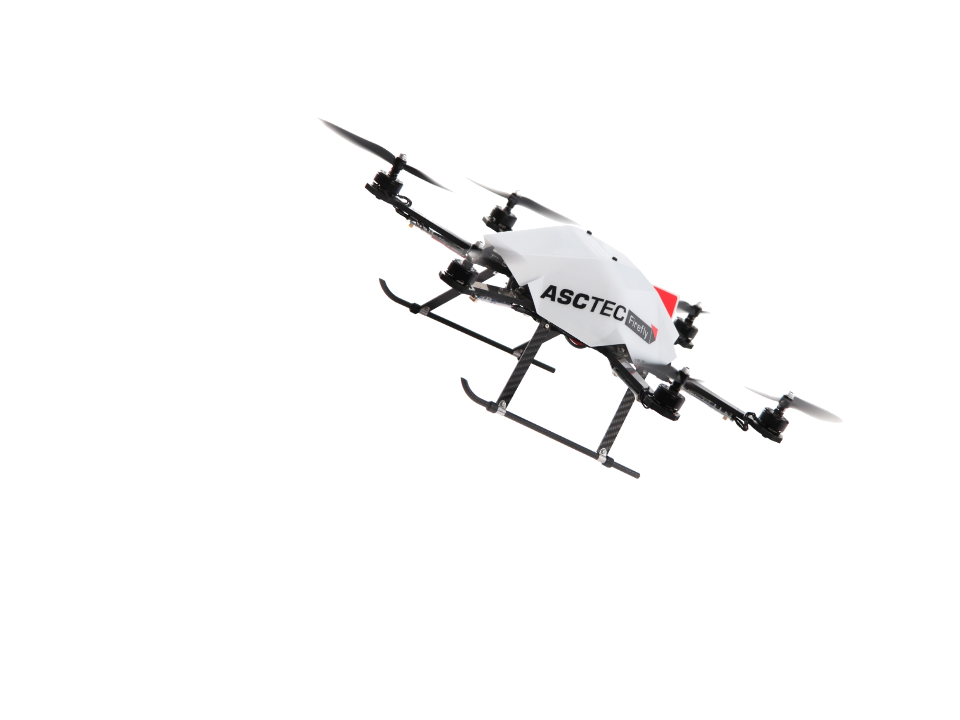
\includegraphics[width=0.6\textwidth]{images/drone.png}
  \end{figure}

\end{frame}

\begin{frame}[plain,c]
  \begin{center}
    Thank you for your attention,\\
    Any question?
  \end{center}
\end{frame}

\begin{frame}[noframenumbering]{Gyroscope bias estimation}
  \begin{figure}[h!]
    \centering

    \begin{subfigure}[b]{0.78\textwidth}
      \caption{Optimized Closed-form solution}
      \resizebox{0.45\textwidth}{!}{% This file was created by matlab2tikz.
% Minimal pgfplots version: 1.3
%
%The latest updates can be retrieved from
%  http://www.mathworks.com/matlabcentral/fileexchange/22022-matlab2tikz
%where you can also make suggestions and rate matlab2tikz.
%
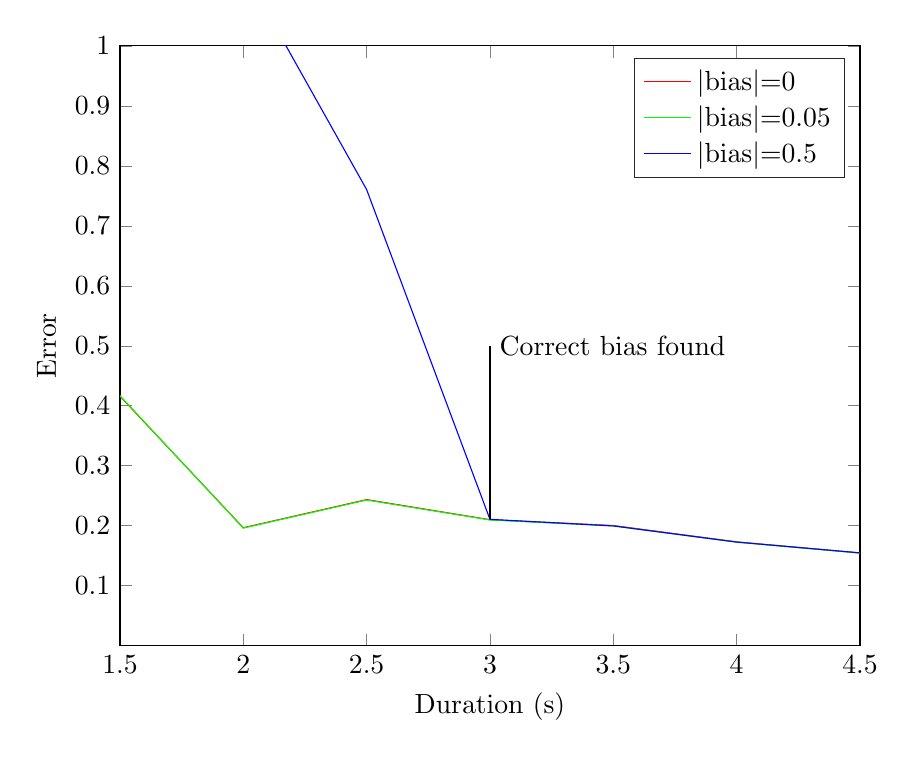
\begin{tikzpicture}

\begin{axis}[%
width=3.7in,
height=3in,
at={(1.751579in,1.09421in)},
scale only axis,
xmin=1.5,
xmax=4.5,
xlabel={Duration (s)},
ytick={0.1,0.2,...,1,1.1},
xtick={1.5,2,...,4,4.5},
ymin=0,
ymax=1,
ylabel={ Error},
legend style={legend cell align=left,align=left,draw=white!15!black}
]
\addplot [color=red,solid]
  table[row sep=crcr]{%
1.5	0.416014163169207\\
2	0.196683554909346\\
2.5	0.243582740699315\\
3	0.210126115008794\\
3.5	0.200403399493516\\
4	0.173117481975929\\
4.5	0.1547038991148\\
};
\addlegendentry{\textbar bias\textbar =0};

\addplot [color=green,solid]
  table[row sep=crcr]{%
1.5	0.41691124744351\\
2	0.196085518742207\\
2.5	0.242845859433578\\
3	0.209595541753857\\
3.5	0.199692504930268\\
4	0.172636924048922\\
4.5	0.154506893070617\\
};
\addlegendentry{\textbar bias\textbar =0.05};

\addplot [color=blue,solid]
  table[row sep=crcr] ~
      \resizebox{0.45\textwidth}{!}{% This file was created by matlab2tikz.
% Minimal pgfplots version: 1.3
%
%The latest updates can be retrieved from
%  http://www.mathworks.com/matlabcentral/fileexchange/22022-matlab2tikz
%where you can also make suggestions and rate matlab2tikz.
%
\definecolor{mycolor1}{rgb}{0.00000,0.44700,0.74100}%
%
\begin{tikzpicture}



\begin{axis}[%
width=4.6in,
height=1in,
at={(0in,3in)},
scale only axis,
xmin=1.5,
xmax=4.5,
xlabel={Duration (s)},
ytick={-0.05,0.0276,0.05},
ymin=-0.06,
ymax=0.06,
xtick={1.5, 2,...,4, 4.5},
ylabel={Bias (rad/s)}
]
\addplot [color=mycolor1,solid,forget plot]
  table[row sep=crcr]{%
1.91728659346996	0.072\\
2	0.0332103321872858\\
2.5	0.025037245454736\\
3	0.0321581893592385\\
3.5	0.027530467500012\\
4	0.0241138134913708\\
4.5	0.0280167461197849\\
};
\draw[line width=2pt,loosely dotted]  (1.5,0.0276 ) -- (4.5,0.0276);
\end{axis}


\begin{axis}[%
width=4.6in,
height=1in,
at={(0in,1.5in)},
scale only axis,
xmin=1.5,
xmax=4.5,
xlabel={Duration (s)},
ymin=-0.06,
ymax=0.06,
xtick={1.5, 2,...,4, 4.5},
ytick={-0.05,-0.0024,0.05},
ylabel={Bias (rad/s)}
]
\addplot [color=mycolor1,solid,forget plot]
  table[row sep=crcr]{%
1.73915180031747	-0.072\\
2	-0.00171936386040559\\
2.5	-0.00299882445661285\\
3	0.00306235287226103\\
3.5	-0.00341664285341729\\
4	-0.00756449922739225\\
4.5	-0.00255081057036582\\
};
\draw[line width=2pt,loosely dotted]  (1.5,-0.0024) -- (4.5,-0.0024);
\end{axis}

\begin{axis}[%
width=4.6in,
height=1in,
at={(0in,0in)},
scale only axis,
xmin=1.5,
xmax=4.5,
xlabel={Duration (s)},
ymin=-0.06,
ymax=0.06,
xtick={1.5, 2,...,4, 4.5},
ytick={-0.05,0.0417},
ylabel={ Bias (rad/s)}
]
\addplot [color=mycolor1,solid,forget plot]
  table[row sep=crcr]
    \end{subfigure}

    \begin{subfigure}[b]{0.40\textwidth}
      \caption{Original Closed-form solution}
      \resizebox{\textwidth}{!}{% This file was created by matlab2tikz.
% Minimal pgfplots version: 1.3
%
%The latest updates can be retrieved from
%  http://www.mathworks.com/matlabcentral/fileexchange/22022-matlab2tikz
%where you can also make suggestions and rate matlab2tikz.
%
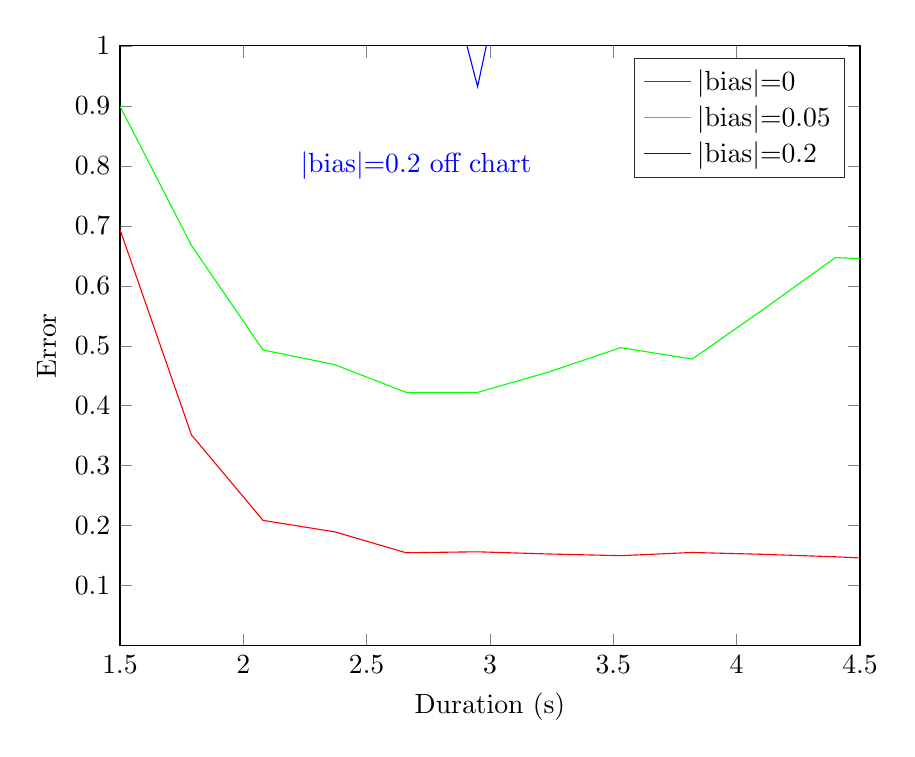
\begin{tikzpicture}

\begin{axis}[%
width=3.7in,
height=3in,
at={(1.751579in,1.09421in)},
scale only axis,
unbounded coords=jump,
xmin=1.5,
xmax=4.5,
xlabel={Duration (s)},
ytick={0.1,0.2,...,1,1.1},
xtick={1.5,2,...,4,4.5},
ymin=0,
ymax=1,
ylabel={Error },
title style={font=\bfseries},
legend style={legend cell align=left,align=left,draw=white!15!black}
]
\addplot [color=red,solid]
  table[row sep=crcr]{%
1.5	0.69385799743164\\
1.79	0.351400106646042\\
2.08	0.208972359940106\\
2.37	0.189904693757416\\
2.66	0.155031673380865\\
2.95	0.156603969287685\\
3.24	0.152939916596076\\
3.53	0.150155750111395\\
3.82	0.15549617974511\\
4.11	0.152358693836919\\
4.4	0.148302651272463\\
4.69	0.142615204897316\\
};
\addlegendentry{\textbar bias\textbar =0};

\addplot [color=green,solid]
  table[row sep=crcr]{%
1.5	0.899343688689263\\
1.79	0.6670895311607\\
2.08	0.492994031916181\\
2.37	0.468605658830025\\
2.66	0.422315774521047\\
2.95	0.422348108072392\\
3.24	0.456442867280175\\
3.53	0.496882747914263\\
3.82	0.477797052531491\\
4.11	0.561139746296675\\
4.4	0.646949430497149\\
4.69	0.642082595006945\\
};
\addlegendentry{\textbar bias\textbar =0.05};

\addplot [color=blue,solid]
  table[row sep=crcr]
    \end{subfigure}

  \end{figure}
\end{frame}

\begin{frame}[noframenumbering]{Numerical stability}

  \begin{columns}
    \begin{column}{.5\textwidth}
    {\small
    \[
    \left[
      \begin{array}{lcl}
        S_j &=& \lambda_1^1\mu_1^1 - V t_j - G \frac{t_j^2}{2} - \lambda^1_j \mu^1_j\\
        0_3 &=& \lambda_1^1\mu_1^1 - \lambda_j^1\mu_j^1 - \lambda_1^i\mu_1^i + \lambda^i_j \mu^i_j
      \end{array}
      \right.
      \]
    }
    \end{column}
    \vrule{}
    \begin{column}{.5\textwidth}
    {\small
    \[
    S_j = \lambda_1^i\mu_1^i - V t_j - G \frac{t_j^2}{2} - \lambda^i_j \mu^i_j
    \]
    }
    \end{column}
  \end{columns}

  \begin{figure}[h!]
    \centering
    \resizebox{0.5\textwidth}{!}{% This file was created by matlab2tikz.
% Minimal pgfplots version: 1.3
%
%The latest updates can be retrieved from
%  http://www.mathworks.com/matlabcentral/fileexchange/22022-matlab2tikz
%where you can also make suggestions and rate matlab2tikz.
%
\definecolor{mycolor1}{rgb}{0,1,0}%
%
\begin{tikzpicture}

\begin{axis}[%
width=4.5in,
height=3.7in,
at={(1.751579in,1.09421in)},
scale only axis,
xmin=1.5,
xmax=4.5,
xlabel={Duration (s)},
ymin=0,
ymax=1,
ylabel={Error},
xtick={1.5,2,...,4,4.5},
ytick={0.1,0.2,...,1,1.1},
legend style={legend cell align=left,align=left,draw=white!15!black}
]
\addplot [color=blue,solid]
  table[row sep=crcr]{%
1.5	0.762801178696159\\
2	0.490854841841618\\
2.5	0.460758656914928\\
3	0.481813646472708\\
3.5	0.461642438720163\\
4	0.437968480311408\\
4.5	0.409852108955419\\
};
\addlegendentry{lambda};

\addplot [color=red,solid]
  table[row sep=crcr]{%
1.5	0.897783065827637\\
2	0.625026337752138\\
2.5	0.594488594286172\\
3	0.625761539018411\\
3.5	0.555488396593806\\
4	0.465559666180634\\
4.5	0.362061397104667\\
};
\addlegendentry{speed};

\addplot [color=mycolor1,solid]
  table[row sep=crcr]{%
1.5	0.152942570020578\\
2	0.0888439460940633\\
2.5	0.0761934019897938\\
3	0.069897164835093\\
3.5	0.0546837789020217\\
4	0.0447432430773695\\
4.5	0.0350875815151695\\
};
\addlegendentry{gravity};

\addplot [color=blue,dashed,forget plot]
  table[row sep=crcr]{%
1.5	0.480537472096306\\
2	0.196912371216785\\
2.5	0.155592643916494\\
3	0.127828533647364\\
3.5	0.154812585819844\\
4	0.146932044398348\\
4.5	0.141815233170712\\
};
\addplot [color=red,dashed,forget plot]
  table[row sep=crcr]{%
1.5	0.561708970792134\\
2	0.300202332539254\\
2.5	0.286604210592777\\
3	0.233549680819569\\
3.5	0.237067972551295\\
4	0.228623572747178\\
4.5	0.229259217854787\\
};
\addplot [color=mycolor1,dashed,forget plot]
  table[row sep=crcr]
  \end{figure}

\end{frame}

%% \begin{document}
%% \title{Simple Beamer Class}
%% \author{Sascha Frank}
%% \date{\today}

%% \frame{\titlepage}

%% \frame{\frametitle{Table of contents}\tableofcontents}



\end{document}
